
%!TEX TS-program = pdflatex
%!TEX encoding = UTF-8 Unicode

%This is a simple template for a LaTeX document using the "article" class.
%See "book", "report", "letter" for other types of document.

\documentclass[12pt]{article} % use larger type; default would be 10pt

\usepackage[utf8]{inputenc} % set input encoding (not needed with XeLaTeX)

%%% Examples of Article customizations
%These packages are optional, depending whether you want the features they provide.
%See the LaTeX Companion or other references for full information.

%%% PAGE DIMENSIONS
\usepackage{geometry} % to change the page dimensions
\geometry{a4paper} % or letterpaper (US) or a5paper or....
%\geometry{margins=2in} % for example, change the margins to 2 inches all round
%\geometry{landscape} % set up the page for landscape
%read geometry.pdf for detailed page layout information

\usepackage{graphicx} % support the \includegraphics command and options
%\usepackage[parfill]{parskip} % Activate to begin paragraphs with an empty line rather than an indent

%%% PACKAGES
\usepackage{booktabs} % for much better looking tables
\usepackage{array} % for better arrays (eg matrices) in maths
\usepackage{paralist} % very flexible & customisable lists (eg. enumerate/itemize, etc.)
\usepackage{verbatim} % adds environment for commenting out blocks of text & for better verbatim
\usepackage{spverbatim} % adds environment for commenting out blocks of text & for better verbatim
\usepackage{subfig} % make it possible to include more than one captioned figure/table in a single float
% These packages are all incorporated in the memoir class to one degree or another...
\usepackage{listings}

%%%%%%%%%%%%%%%%%%%%%%%%%%%%%%%
%%%%%%%%%%%%%%%%%%%%%%%%%%%%%%%
%%%%%%%%%%%%%%%%%%%%%%%%%%%%%%%
\usepackage{amsmath} % AMS Math Package
\usepackage{amsthm} % Theorem Formatting
\usepackage{amssymb}	% Math symbols such as \mathbb
\usepackage{graphicx} % Allows for eps images
\usepackage{multicol} % Allows for multiple columns
\renewcommand{\labelenumi}{(\alph{enumi})} % Use letters for enumerate
% \DeclareMathOperator{\Sample}{Sample}
\let\vaccent=\v % rename builtin command \v{} to \vaccent{}
\renewcommand{\v}[1]{\ensuremath{\mathbf{#1}}} % for vectors
\newcommand{\gv}[1]{\ensuremath{\mbox{\boldmath$ #1 $}}} 
% for vectors of Greek letters
\newcommand{\uv}[1]{\ensuremath{\mathbf{\hat{#1}}}} % for unit vector
\newcommand{\abs}[1]{\left| #1 \right|} % for absolute value
\newcommand{\avg}[1]{\left< #1 \right>} % for average
\let\underdot=\d % rename builtin command \d{} to \underdot{}
\renewcommand{\d}[2]{\frac{d #1}{d #2}} % for derivatives
\newcommand{\dd}[2]{\frac{d^2 #1}{d #2^2}} % for double derivatives
\newcommand{\pd}[2]{\frac{\partial #1}{\partial #2}} 
% for partial derivatives
\newcommand{\pdd}[2]{\frac{\partial^2 #1}{\partial #2^2}} 
% for double partial derivatives
\newcommand{\pdc}[3]{\left( \frac{\partial #1}{\partial #2}
 \right)_{#3}} % for thermodynamic partial derivatives
\newcommand{\ket}[1]{\left| #1 \right>} % for Dirac bras
\newcommand{\bra}[1]{\left< #1 \right|} % for Dirac kets
\newcommand{\braket}[2]{\left< #1 \vphantom{#2} \right|
 \left. #2 \vphantom{#1} \right>} % for Dirac brackets
\newcommand{\matrixel}[3]{\left< #1 \vphantom{#2#3} \right|
 #2 \left| #3 \vphantom{#1#2} \right>} % for Dirac matrix elements
\newcommand{\grad}[1]{\gv{\nabla} #1} % for gradient
\let\divsymb=\div % rename builtin command \div to \divsymb
\renewcommand{\div}[1]{\gv{\nabla} \cdot #1} % for divergence
\newcommand{\curl}[1]{\gv{\nabla} \times #1} % for curl
\let\baraccent=\= % rename builtin command \= to \baraccent
\renewcommand{\=}[1]{\stackrel{#1}{=}} % for putting numbers above =
\newtheorem{prop}{Proposition}
\newtheorem{thm}{Theorem}[section]
\newtheorem{lem}[thm]{Lemma}
\theoremstyle{definition}
\newtheorem{dfn}{Definition}
\theoremstyle{remark}
\newtheorem*{rmk}{Remark}
%%%%%%%%%%%%%%%%%%%%%%%%%%%%%%%
%%%%%%%%%%%%%%%%%%%%%%%%%%%%%%%
%%%%%%%%%%%%%%%%%%%%%%%%%%%%%%%

\usepackage{wrapfig} %Para insertar imágenes dentro del texto
\usepackage{graphicx} %Para insertar imágenes
\usepackage{appendix}  %Para poner un apéndice
\usepackage{hyperref}



%%% HEADERS & FOOTERS
\usepackage{fancyhdr} % This should be set AFTER setting up the page geometry
\pagestyle{fancy} % options: empty , plain , fancy
\renewcommand{\headrulewidth}{0pt} % customise the layout...
\lhead{}\chead{}\rhead{}
\lfoot{}\cfoot{\thepage}\rfoot{}

%%% SECTION TITLE APPEARANCE
\usepackage{sectsty}
\allsectionsfont{\sffamily\mdseries\upshape} % (See the fntguide.pdf for font help)
% (This matches ConTeXt defaults)

%%% ToC (table of contents) APPEARANCE
\usepackage[nottoc,notlof,notlot]{tocbibind} % Put the bibliography in the ToC
\usepackage[titles,subfigure]{tocloft} % Alter the style of the Table of Contents
\renewcommand{\cftsecfont}{\rmfamily\mdseries\upshape}
\renewcommand{\cftsecpagefont}{\rmfamily\mdseries\upshape} % No bold!

%Para poder elegir el tamaño de los márgenes
\usepackage{anysize}

%\input{header.tex}

%%%Para poner en castellano los titulos de las secciones
\renewcommand{\contentsname}{Contenidos}
\renewcommand{\listfigurename}{Figuras}
\renewcommand{\listtablename}{Tablas}
\renewcommand{\refname}{Bibliograf\'ia}
\renewcommand{\tablename}{Tabla}
\renewcommand{\figurename}{Figura}
\renewcommand{\appendixpagename}{Apéndices} 
%%% END Article customizations

%%% The "real" document content comes below...

%Los siguientes paquetes son para que no corte las palabras
\pretolerance=2000
\tolerance=3000 


\usepackage{geometry}
 \geometry{
 a4paper,
 left=15mm,
 right=10mm,
 top=20mm,
 bottom=20mm,
 }


%AQUI EMPIEZAN LAS MODIFICACIONES DEPENDIENDO DEL TRABAJO


\begin{document}
\title{Colisión de un sistema con disco con un satélite esférico con relación de masas 10:1 en una órbita polar}
\section*{Condiciones iniciales}

\paragraph{Unidades}
Se usa un sistema de unidades en cual G = 1, [M] = $10^{11} M_{Sol}$, [l] = 1kpc $\implies$ [v]= 655.85 km/s [t] = 1.49My


\subsection*{los modelos individuales}

\begin{description}
\item Uso los modelos esféricos y con disco obtenidos en las prácticas anteriores (ya escalados con masa total 1)
\item El modelo elíptico obtenido con isomodr4 (Smulders \& Balcells) tiene 50000 particulas(10000 en el bulbo y 40000 en el halo). El halo usa un modelo Hernquist y el bulbo un modelo Jaffe, la relacion de masas es $M_{halo}:M_{bulbo} = 3:1$
\item La galáxia con disco(espiral) obtenido con el modelo Widrow \& Dubinski tiene 20000 particulas (8000 en el disco, 4000 en el bulbo, 8000 en el halo) 
\item El modelo elíptico se escala a una masa total 0.1 (cuando se escalan los modelos el radio se escala también para que se cumpla la relación: $\frac{R_1}{R_2} = \sqrt{\frac{M_1}{M_2}}$). Es mejor escalar el segundo modelo antes de ponerlos en órbita usando \textbf{scale} y no especificando estas relaciones en setorbdat porque parece que no funciona
\item los parámetros que se van a configurar para tree500 en TREEPAR: dt y eps dependen de estos modelos iniciales
\begin{description}
\item En la práctica usamos valores máximos para  dt = $\frac{1}{20} t_{cruce} = \frac{1}{20} \sqrt{\frac{R^3}{M}}$ y eps = $0.2 R$ donde R es el radio de media masa y M es la media masa de la parte luminos elijiendo los valores mas pequeños de los 2 modelos
\item
\small
\begin{verbatim}
 nora>> data two.xvp 1
 getmodel>> model :            1
 xvpread>> Reading    70000 particles from model     0.0000 of file :two.xvp                                 
  getmodel:: nbods =   70000.0000       iteration =   300.000000       time =   16.0200100    
 nora>> list head 100 110
   1.00000000    
   5.00000000    
   8000.00000    
   1.02271779E-05
   12000.0000    
   7.43265036E-06
   20000.0000    
   1.10622786E-04
   30000.0000    
   2.49999994E-06
   70000.0000    
 nora>> bodsrange 1 12000
 nora>> Rm 100
#
#FILE two.xvp    MODEL     1                                                    
#PART       1-  12000  VIEW    0.0,   0.0  RMAX 100.0  SLIT  -0.0, 0.0,*****    
#totm =  1.116E-01
#FRM :      0.01     0.02     0.05     0.10     0.20     0.30     0.40     0.50
#Rm  :  2.23E+00 2.29E+00 2.31E+00 2.34E+00 2.40E+00 2.46E+00 2.53E+00 2.59E+00
#FRM :      0.60     0.70     0.80     0.90     0.95     0.98     0.99     1.00
#Rm  :  2.65E+00 2.71E+00 2.77E+00 2.84E+00 2.87E+00 2.89E+00 2.89E+00 1.00E+15
 nora>> bodsrange 30001 40000
 nora>> Rm 100
#
#FILE two.xvp    MODEL     1                                                    
#PART   30001-  40000  VIEW    0.0,   0.0  RMAX 100.0  SLIT  -0.0, 0.0,*****    
#totm =  1.875E-02
#FRM :      0.01     0.02     0.05     0.10     0.20     0.30     0.40     0.50
#Rm  :  1.27E+00 1.48E+00 1.82E+00 1.99E+00 2.30E+00 2.40E+00 2.50E+00 2.60E+00
#FRM :      0.60     0.70     0.80     0.90     0.95     0.98     0.99     1.00
#Rm  :  2.70E+00 2.79E+00 2.89E+00 3.37E+00 3.61E+00 4.16E+00 4.42E+00 1.00E+15

\end{verbatim}

\normalsize
\item $R_1$ = 2.59E+00, $M_1$ = 0.5 * 1.116E-01 $\implies$ $dt_1$ = 0.8822721105537292 y $eps_1$ = 0.518
\item $R_2$ = 2.60E+00, $M_2$ = 0.5 * 1.875E-02 $\implies$ $dt_2$ = 1.5308385501634936 y $eps_2$ = 0.52

\item Con unos valores de dt = 0.8822721105537292 y eps = 0.518 la simulación debería ir bien, elijiendo unos valores mas pequeños la simulación es más realista, pero tardará más (explicación en Clase2.pdf)
\item yo elegí dt = 0.1146314 y eps = 0.276

\end{description}

\end{description}

\subsection*{puesta en órbita}
\paragraph{kepler}
\begin{description}
\item  si cambiamos el parámetro de impacto hay que ejecutar de nuevo kepler con la nueva separación
\item el parámetro nsteps de TREEPAR depende del parámetro Period de la salida de kepler: hay que poner un par de veces el periodo hasta el encuentro de los 2 objetos (El número de periodos de la ejecución = nsteps * dt / Period)
\item elegí separacion = 20, 10 y 5
\item separación \textbf{5}
\begin{verbatim}
BINARY:  M2/M1= 0.10000      SEP.(M2)=  5.000     (VR,VT)=( -0.46904,  0.00000)
         AngMom=  0.0000      P.A.(M2)=   0.00      PHI(V)=   0.05    VZ=  0.000
 a=     5.00  r-peri=   0.00  r-apo=  10.00  b=  0.00  e= 1.000  Period=   66.98
            V-peri=999.999V-apo=  0.000V(Now)=  0.469T(peri)=    6.08
 BOUND LINEAR TRAJECTORY -- at Orbital Phase (TRUE ANOMALY) =   -0.0548
\end{verbatim}
\item Period = 66.98, yo elegí nsteps = 4000 lo que corresponde a 6.845 periodos
\item separación \textbf{10}
\begin{verbatim}
 BINARY:  M2/M1= 0.10000      SEP.(M2)= 10.000     (VR,VT)=( -0.33166,  0.00000)
         AngMom=  0.0000      P.A.(M2)=   0.00      PHI(V)=   0.05    VZ=  0.000
 a=    10.00  r-peri=   0.00  r-apo=  20.00  b=  0.00  e= 1.000  Period=  189.45
            V-peri=999.999V-apo=  0.000V(Now)=  0.332T(peri)=   17.21
 BOUND LINEAR TRAJECTORY -- at Orbital Phase (TRUE ANOMALY) =   -0.0548
\end{verbatim}

\item Period = 189.45, yo elegí nsteps = 10000 lo que corresponde a 6.05 periodos

\item separación \textbf{20}
\begin{verbatim}
 BINARY:  M2/M1= 0.10000      SEP.(M2)= 20.000     (VR,VT)=( -0.23452,  0.00000)
         AngMom=  0.0000      P.A.(M2)=   0.00      PHI(V)=   0.05    VZ=  0.000
 a=    20.00  r-peri=   0.00  r-apo=  40.00  b=  0.00  e= 1.000  Period=  535.83
            V-peri=999.999V-apo=  0.000V(Now)=  0.235T(peri)=   48.68
 BOUND LINEAR TRAJECTORY -- at Orbital Phase (TRUE ANOMALY) =   -0.0548

\end{verbatim}

\item Period = 535.83, yo elegí nsteps = 30000 lo que corresponde a 6.41 periodos

\item La órbita es parabólica(Binary Orbital Eccentricity = 1) y por haber elegido  bound linear encounter = yes VT = 0 y por haber elegido Binary Approaching Pericenter = yes VR $<$ 0
Hay que poner los valores de VR obtenidos en este paso en el fichero setorbdat


\end{description}

\paragraph{setorb}

\begin{description}
\item  si cambiamos el angulo del spin de los objetos relativo al plano de la orbita de los 2 (en particular la orientación del spin)
hay que ejecutar de nuevo setorb 

he elegido valores de theta1 = 90, 60, 270, 240

Los modelos están aliniados en la direccion ox

\end{description}
\newpage

\begin{figure}[!ht]
 \centering
 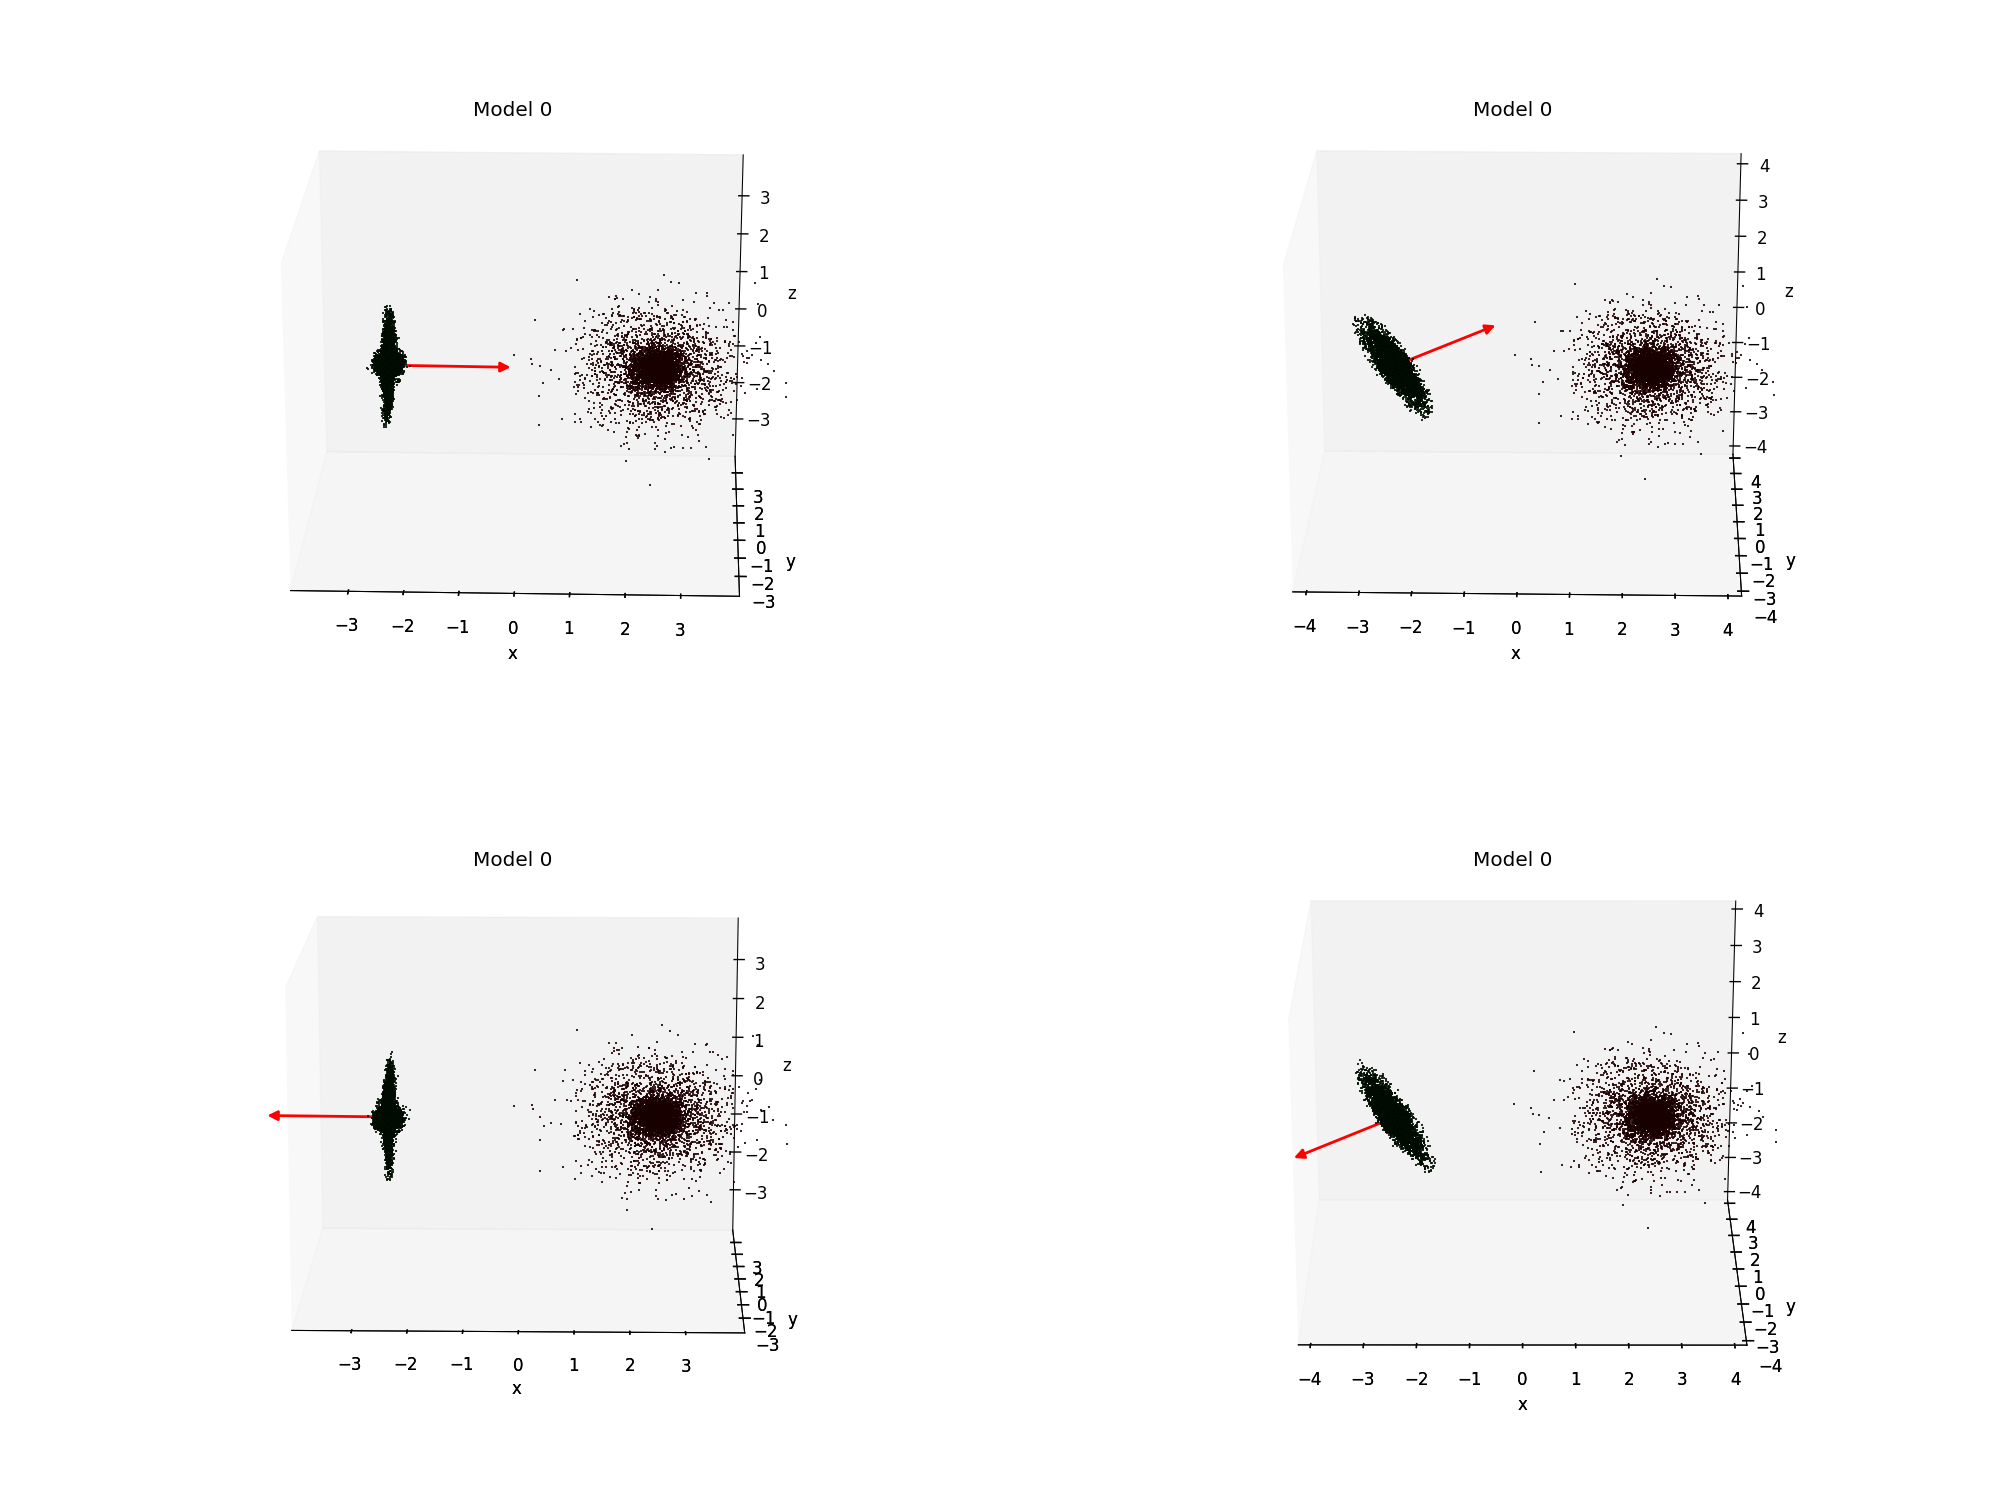
\includegraphics[scale=0.2]{inimod_sep5.png}
 \caption{\emph{Los modelos en el momento inicial(separación = 5), solo la parte luminosa para angulos 90, 60, 270, 240 \\
	Se representa también el vector del momento angular del objeto con disco (el módulo multiplicado por 100) }}
\end{figure}

\begin{figure}[!ht]
 \centering
 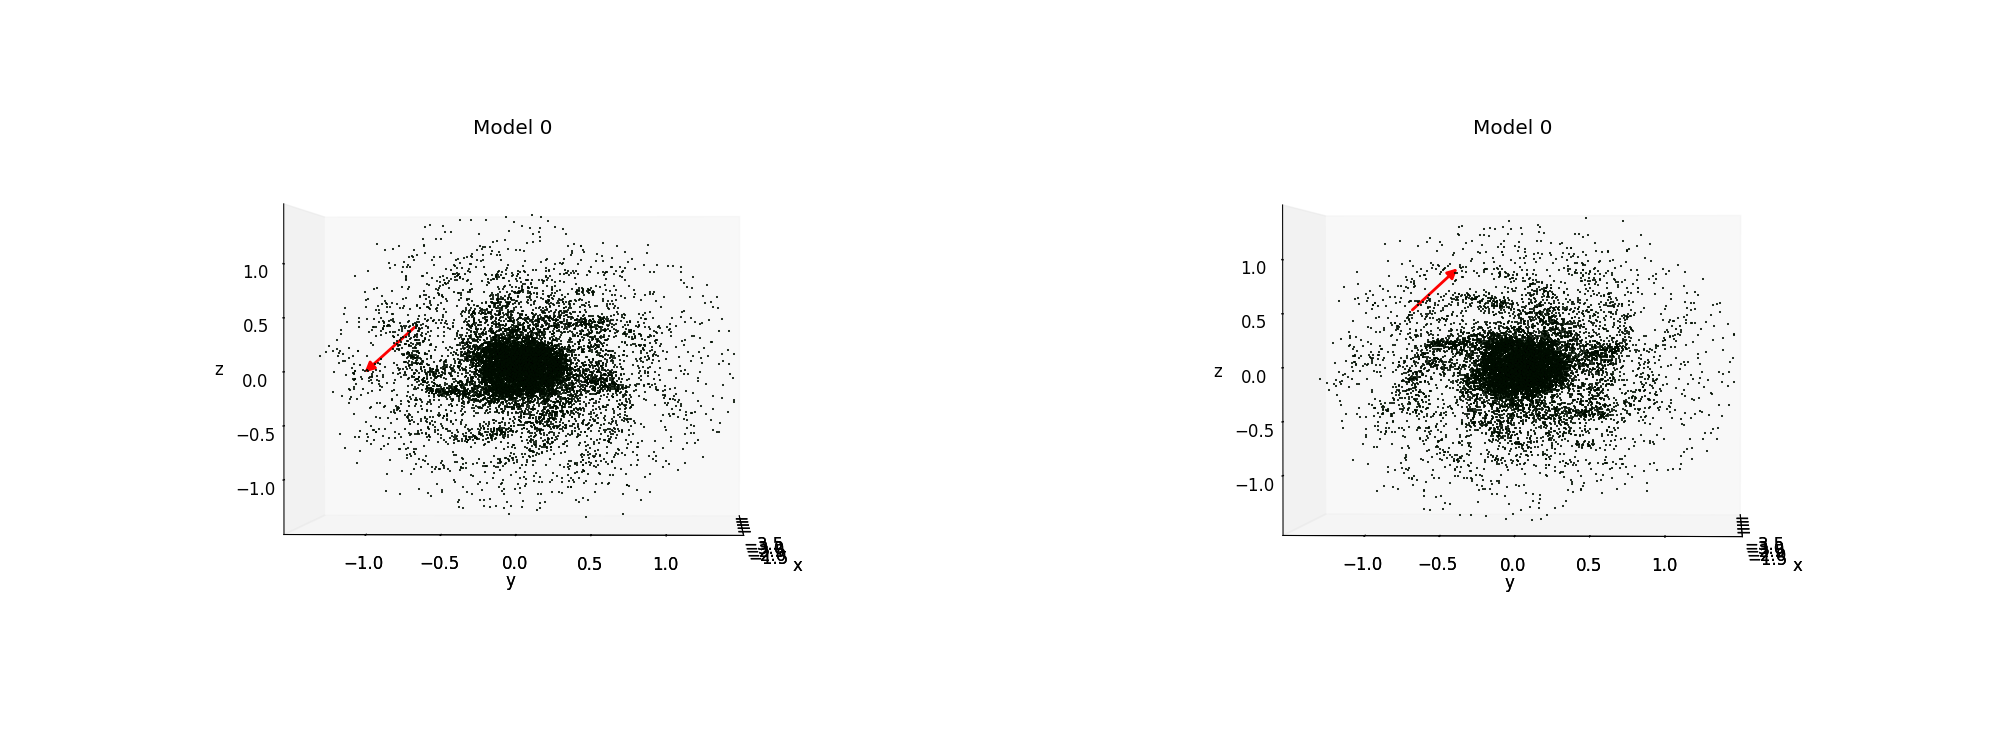
\includegraphics[scale=0.2]{inimoddisco_sep5.png}
 \caption{\emph{El disco y bulbo del primer modelo en el momento inicial visto desde la dirección del otro objeto (y el vector de la velocidad en un punto cualquiera) \\
para los primeros 2 casos (ángulos 90, 60) y para los otros 2 (ángulos 270, 240 - el spin en la otra dirección)}}
\end{figure}





\newpage
\section*{Evolución del modelo}

Los videos de la evolución del modelo(con nombres $sep<SEP>-<DEG>deg-<OBJ>[<PROJAXIS>].mp4 $ donde $<SEP>$ y $<DEG>$ son la separación y angulo theta1 de setorbdat, $<OBJ>$ = 2ob para los 2 objetos(solo bulbo y disco), e para el modelo esférico(solo bulbo) y d para el modelo con disco(solo bulbo y disco) y  $[<PROJAXIS>]$ (opcional) es línea de visión )
están en el repositorio:
\url{https://github.com/beevageeva/simnum2/tree/master/results2/videos}
\small
\begin{verbatim}
sep10-90deg-2ob.mp4 sep10-90deg-dox.mp4 sep10-90deg-doy.mp4 sep10-90deg-e.mp4
sep20-270deg-2ob.mp4 sep20-270deg-dox.mp4 sep20-270deg-doy.mp4 sep20-270deg-e.mp4
sep5-240deg-2ob.mp4 sep5-240deg-dox.mp4 sep5-240deg-doy.mp4 sep5-240deg-eox.mp4
sep5-240deg-eoy.mp4 sep5-270deg-2ob.mp4 sep5-270deg-dox.mp4 sep5-270deg-doy.mp4
sep5-270deg-eox.mp4 sep5-270deg-eoy.mp4 sep5-60deg-2ob.mp4 sep5-60deg-dox.mp4
sep5-60deg-doy.mp4 sep5-60deg-e.mp4 sep5-60deg-eox.mp4 sep5-60deg-eoy.mp4
sep5-90deg-2ob.mp4 sep5-90deg-dox.mp4 sep5-90deg-doy.mp4 sep5-90deg-eox.mp4
sep5-90deg-eoy.mp4
\end{verbatim}

\normalsize



Voy a representar los primeros encuentros (el modelo esférico está atravesando el disco - en caso de la sepración = 5 el primer encuentro pasa en el modelo 1) y el penúltimo (modelo 39)
\tiny Quería representar el último modelo, pero me equivoqué cuando generé las imágenes(para separación = 5 y 10) y no las rehice porque son muy parecidos. Además para separación = 20 la simulación se colgó y solo se se calcularon 236 modelos(en lugar de 300)

\normalsize
La relación entre el número de modelo y el tiempo es: t = noutbod * dt * numModel = 11.46 *  numModel
(en el caso de la separación = 5 hay 41 modelos con numModel = 0..40)



\begin{figure}[!ht]
 \centering
 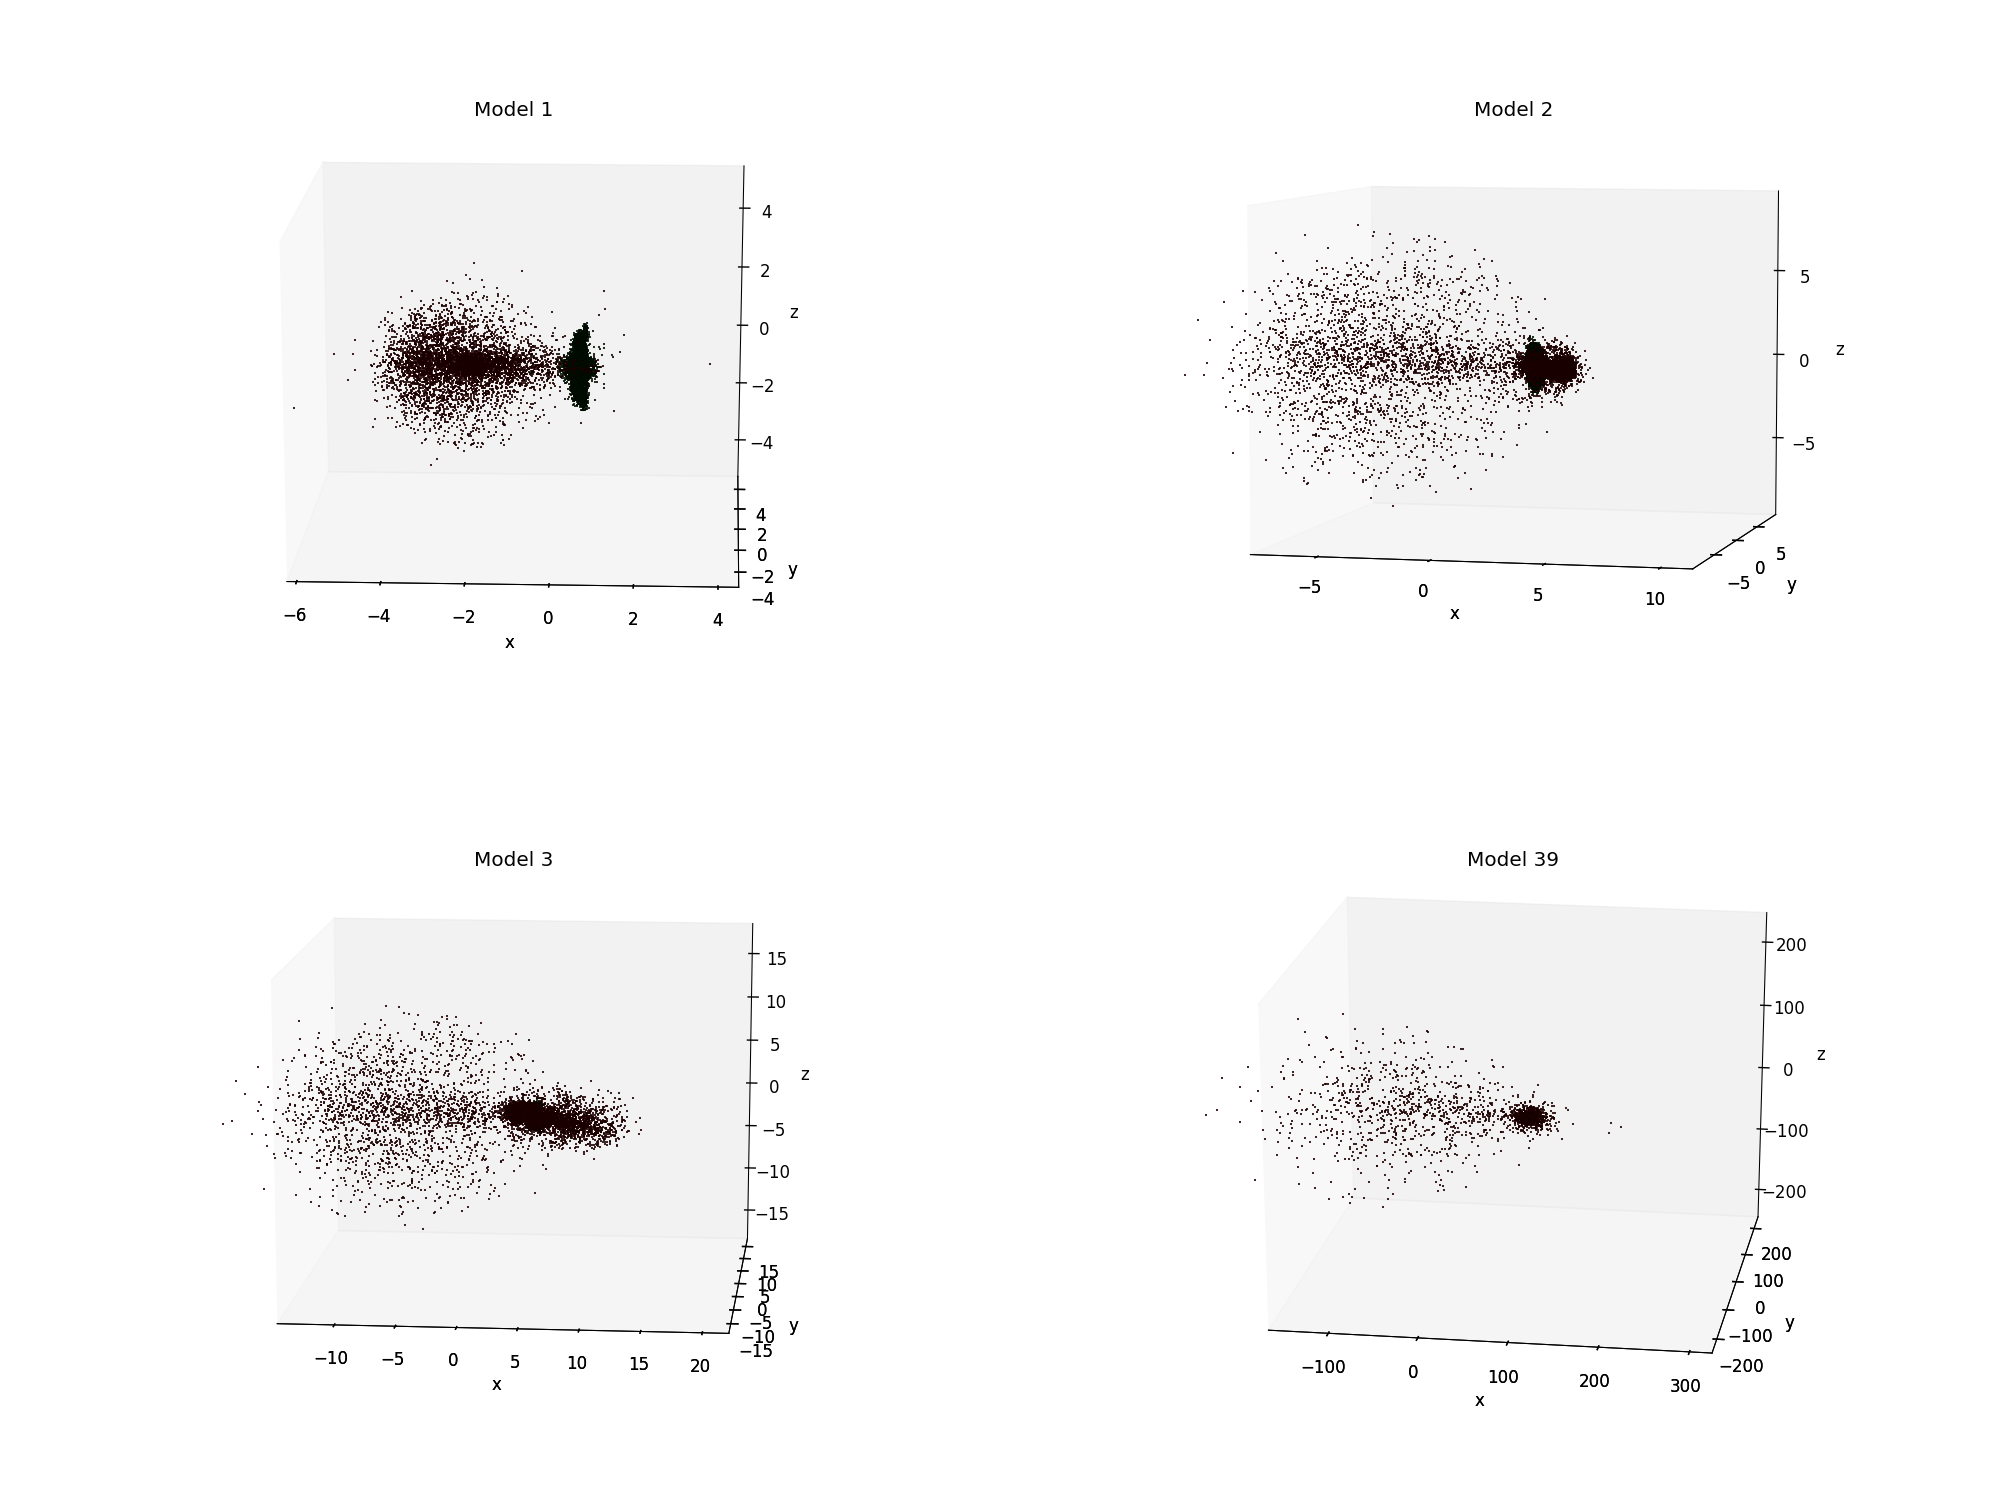
\includegraphics[scale=0.2]{90deg_m_sep5.png}
 \caption{\emph{ ángulo = 90 grados, los 2 objetos(solo parte luminosa) modelo 1,2,3,39 }}
\end{figure}

\begin{figure}[!ht]
 \centering
 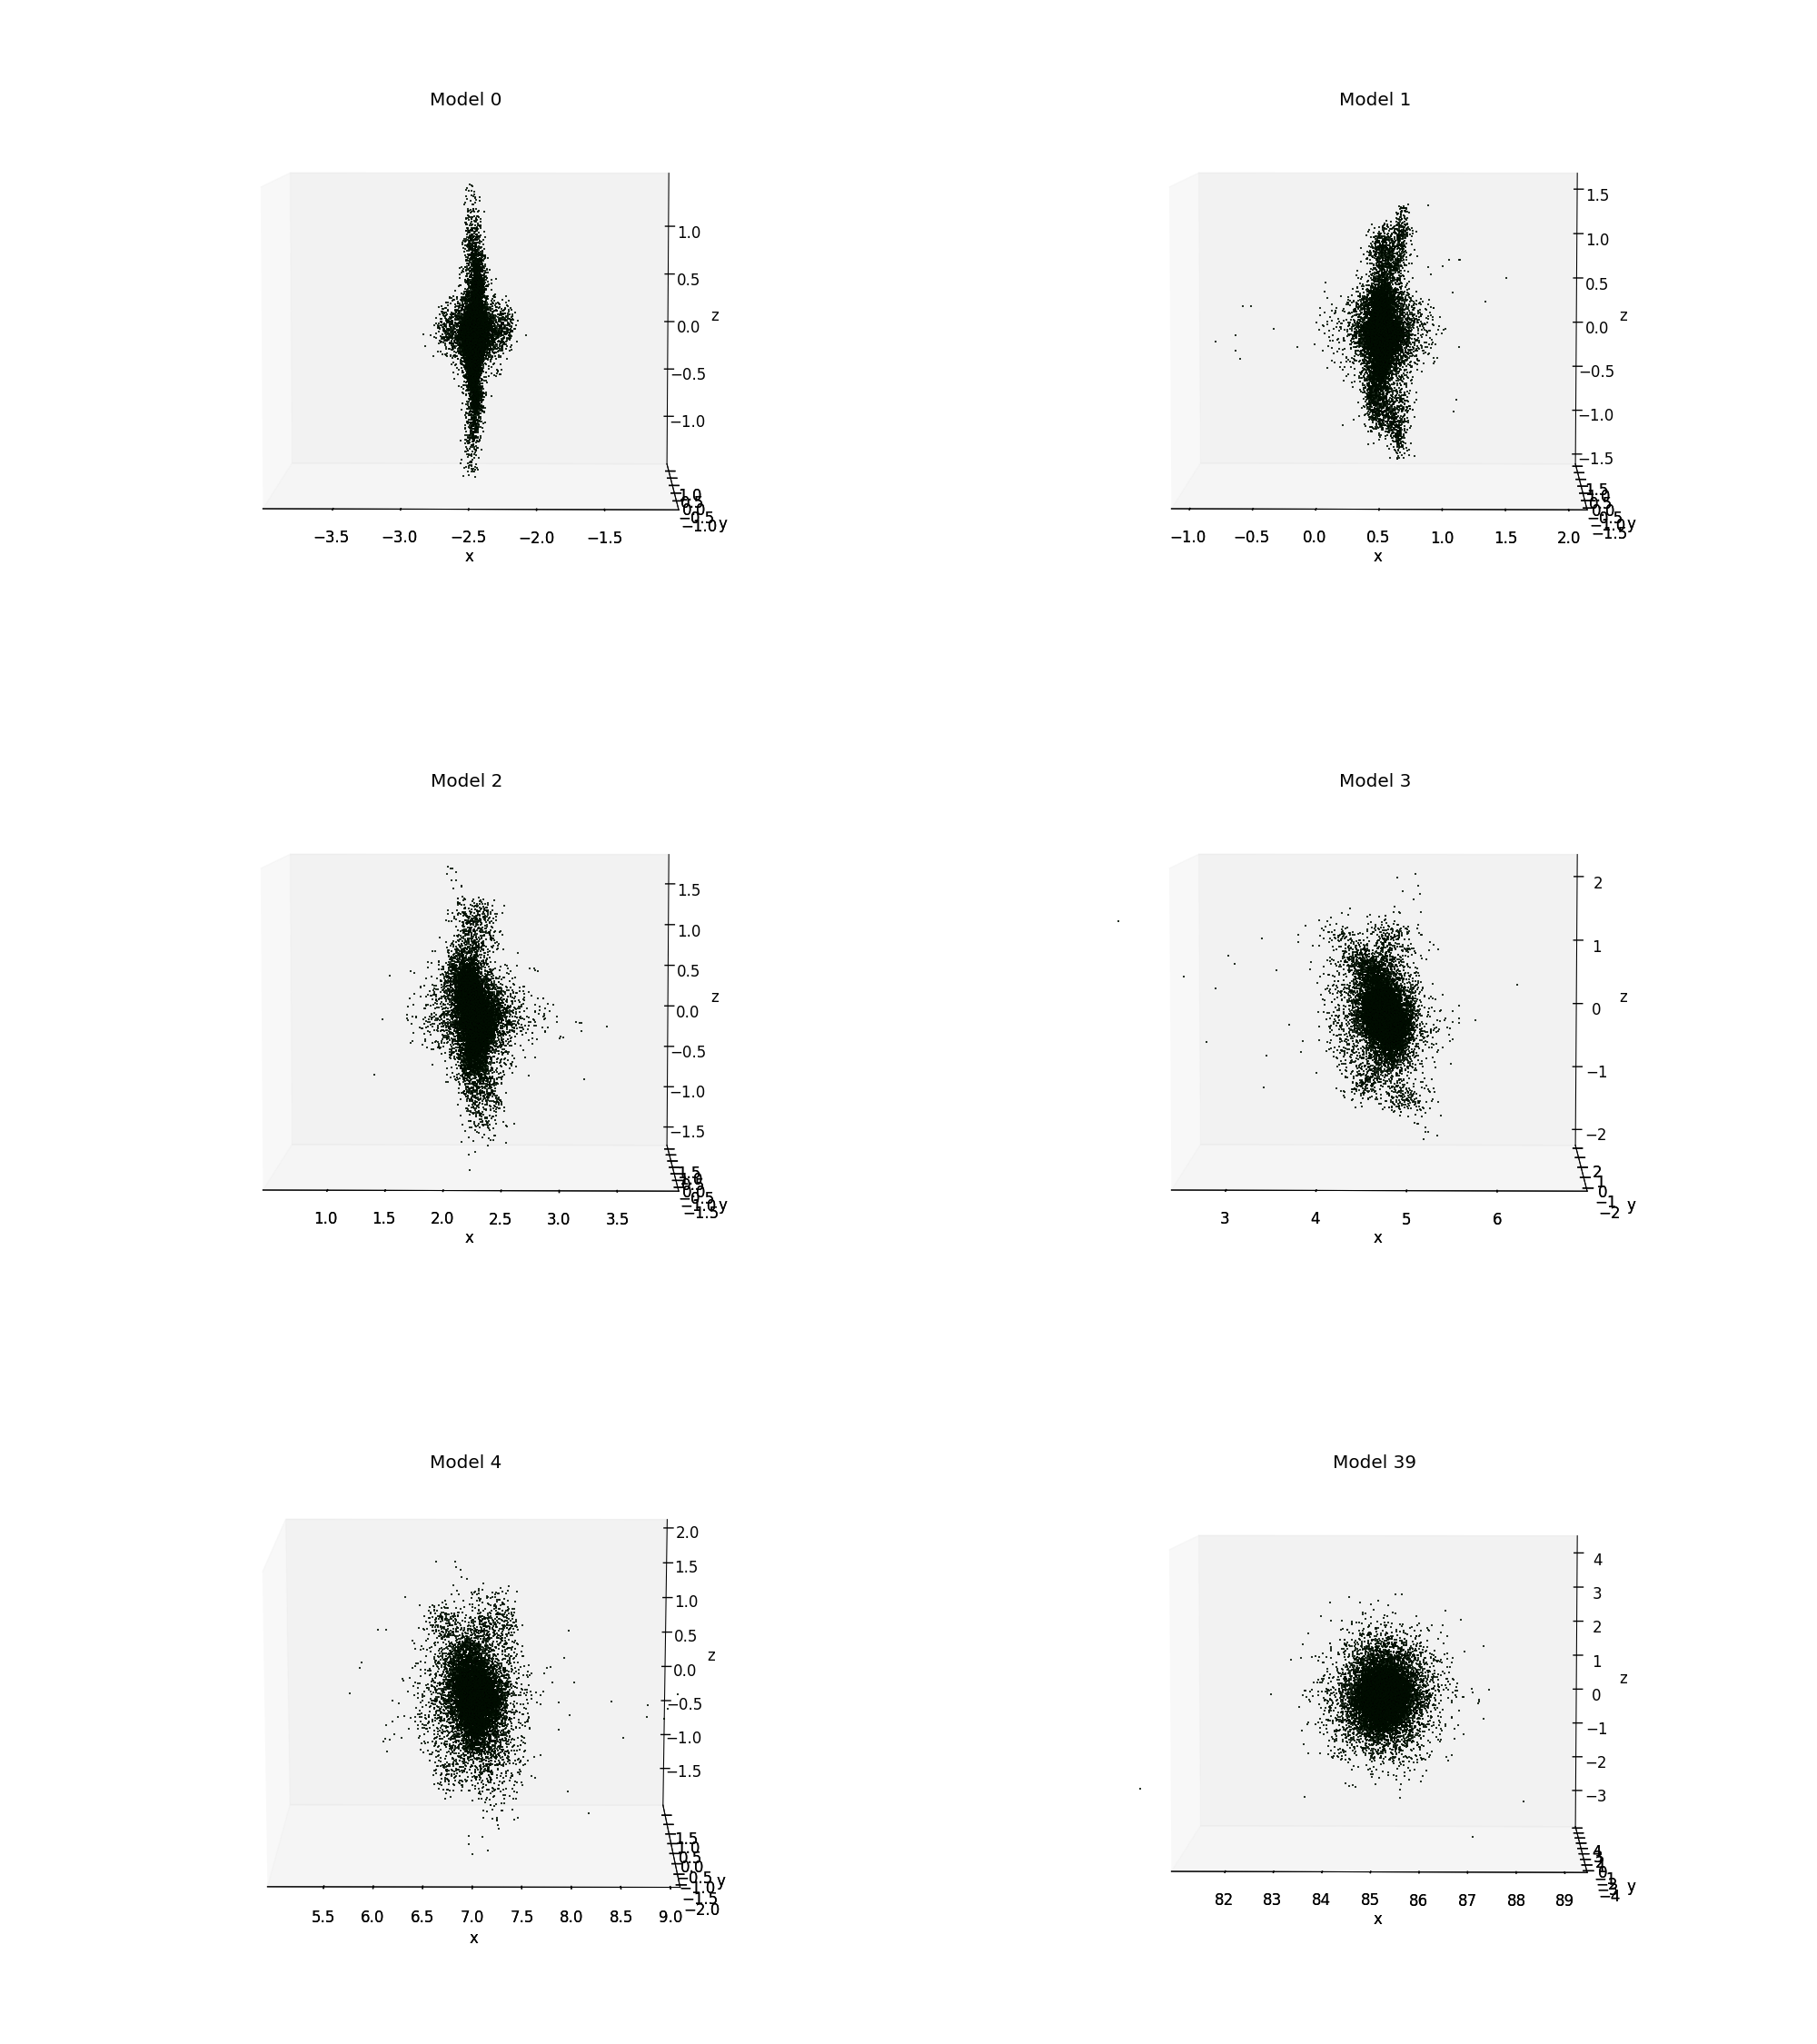
\includegraphics[scale=0.2]{90deg-m-c2y.png}
 \caption{\emph{ ángulo = 90 grados, el objeto con disco visto en la dirección oy(solo parte luminosa) modelo 0,1,2,3,4,39 }}
\end{figure}

\begin{figure}[!ht]
 \centering
 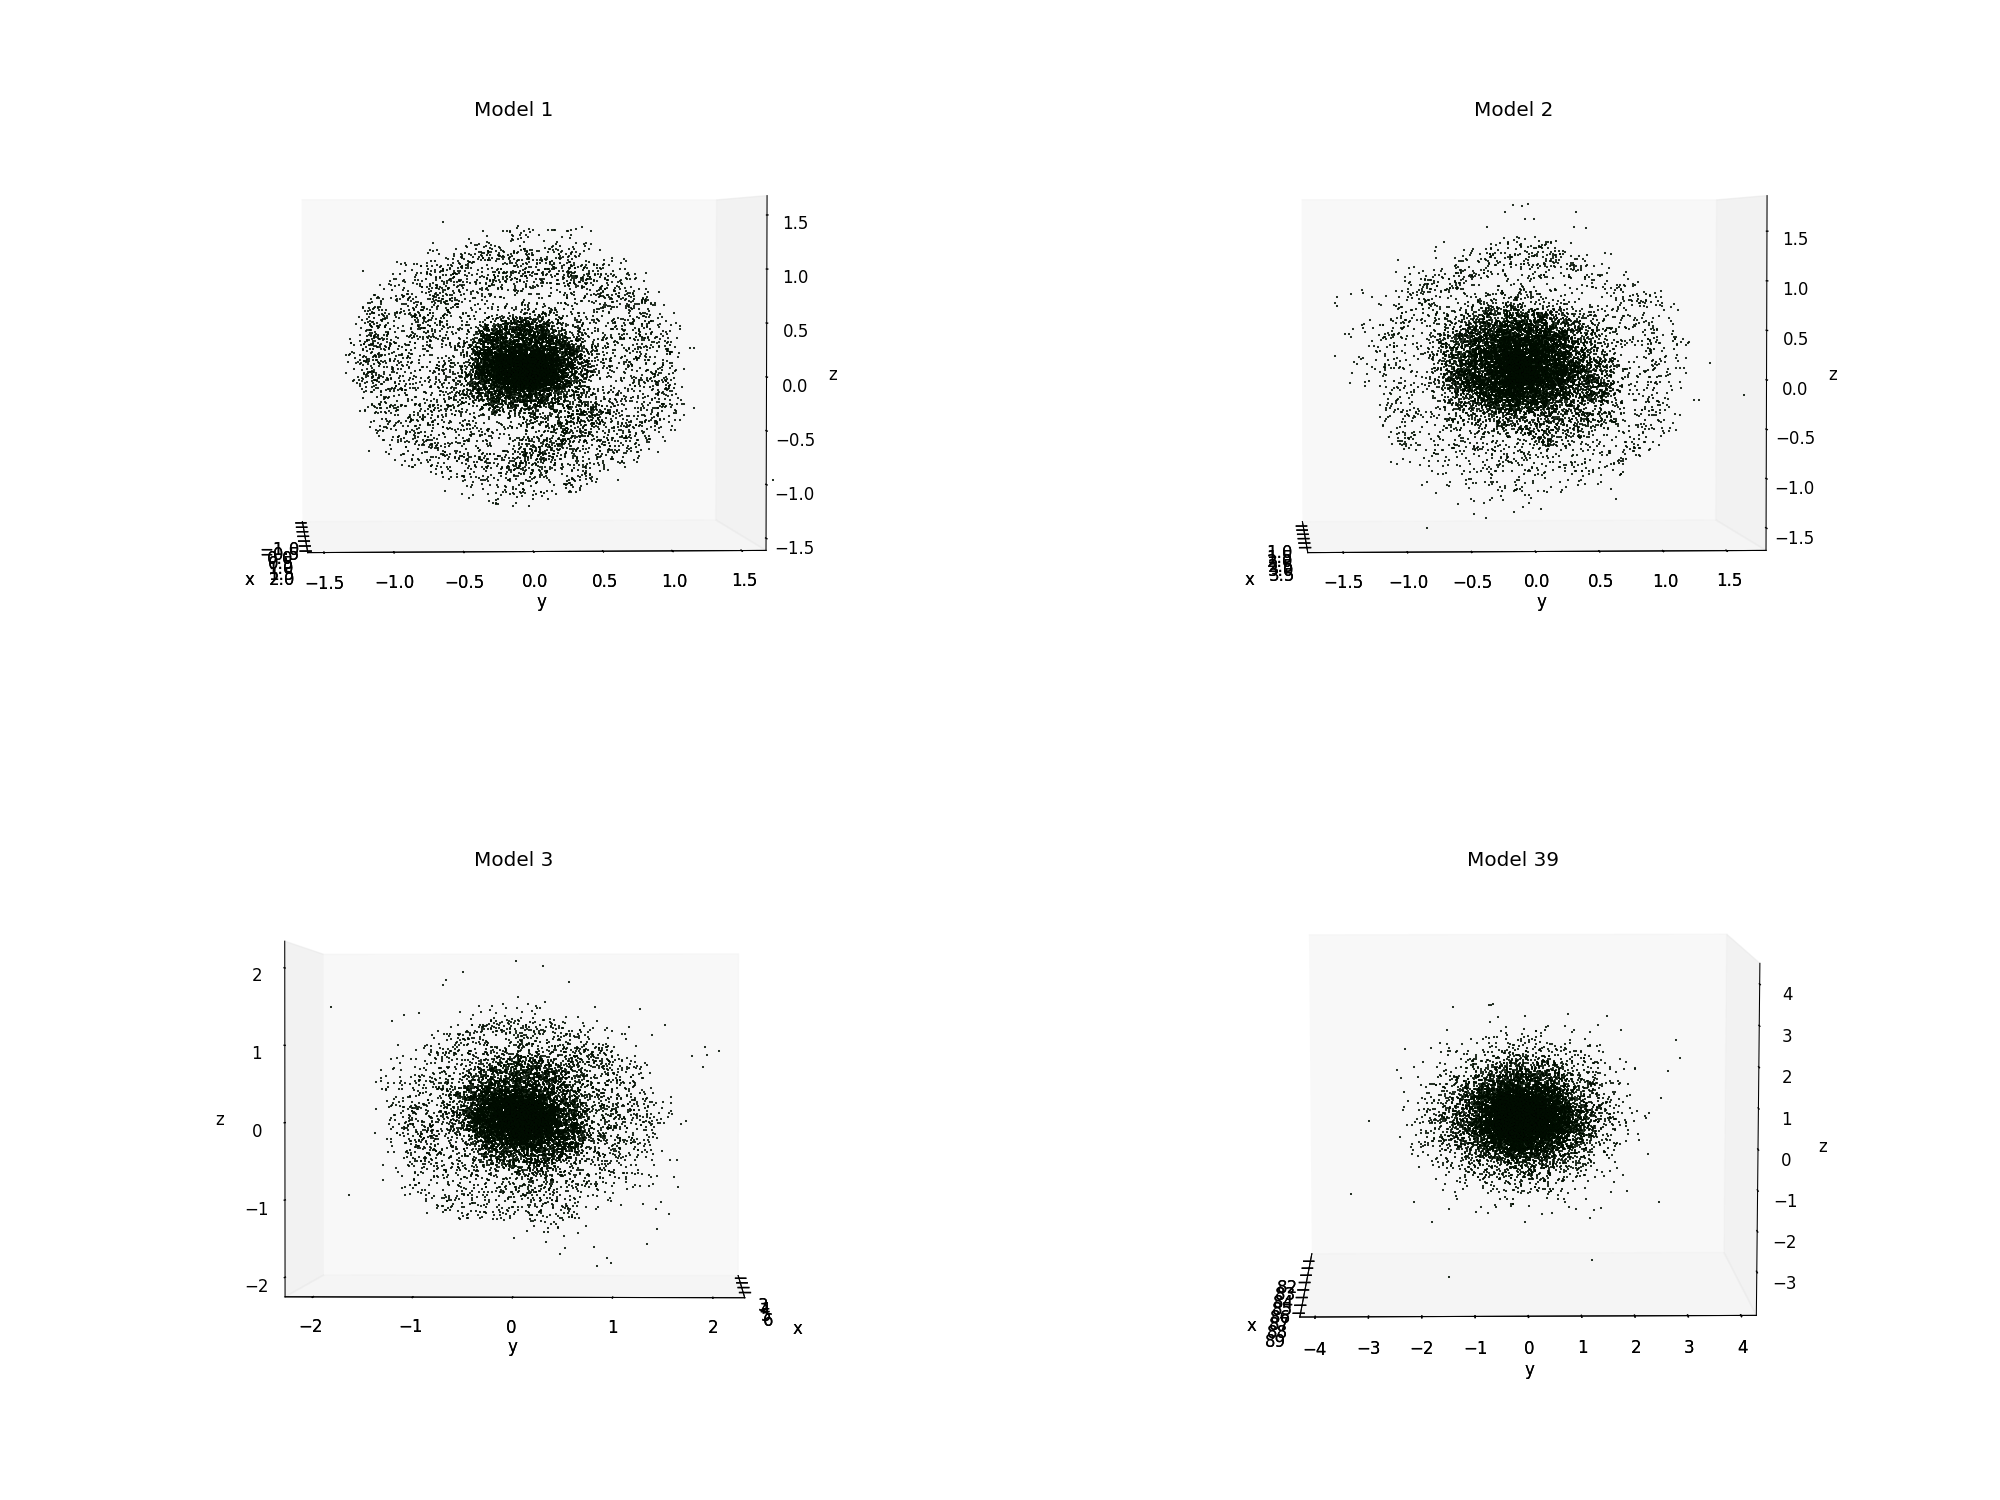
\includegraphics[scale=0.2]{90deg-m-c2.png}
 \caption{\emph{ ángulo = 90 grados, el objeto con disco visto en la dirección ox(solo parte luminosa) modelo 1,2,3,39 }}
\end{figure}

\begin{figure}[!ht]
 \centering
 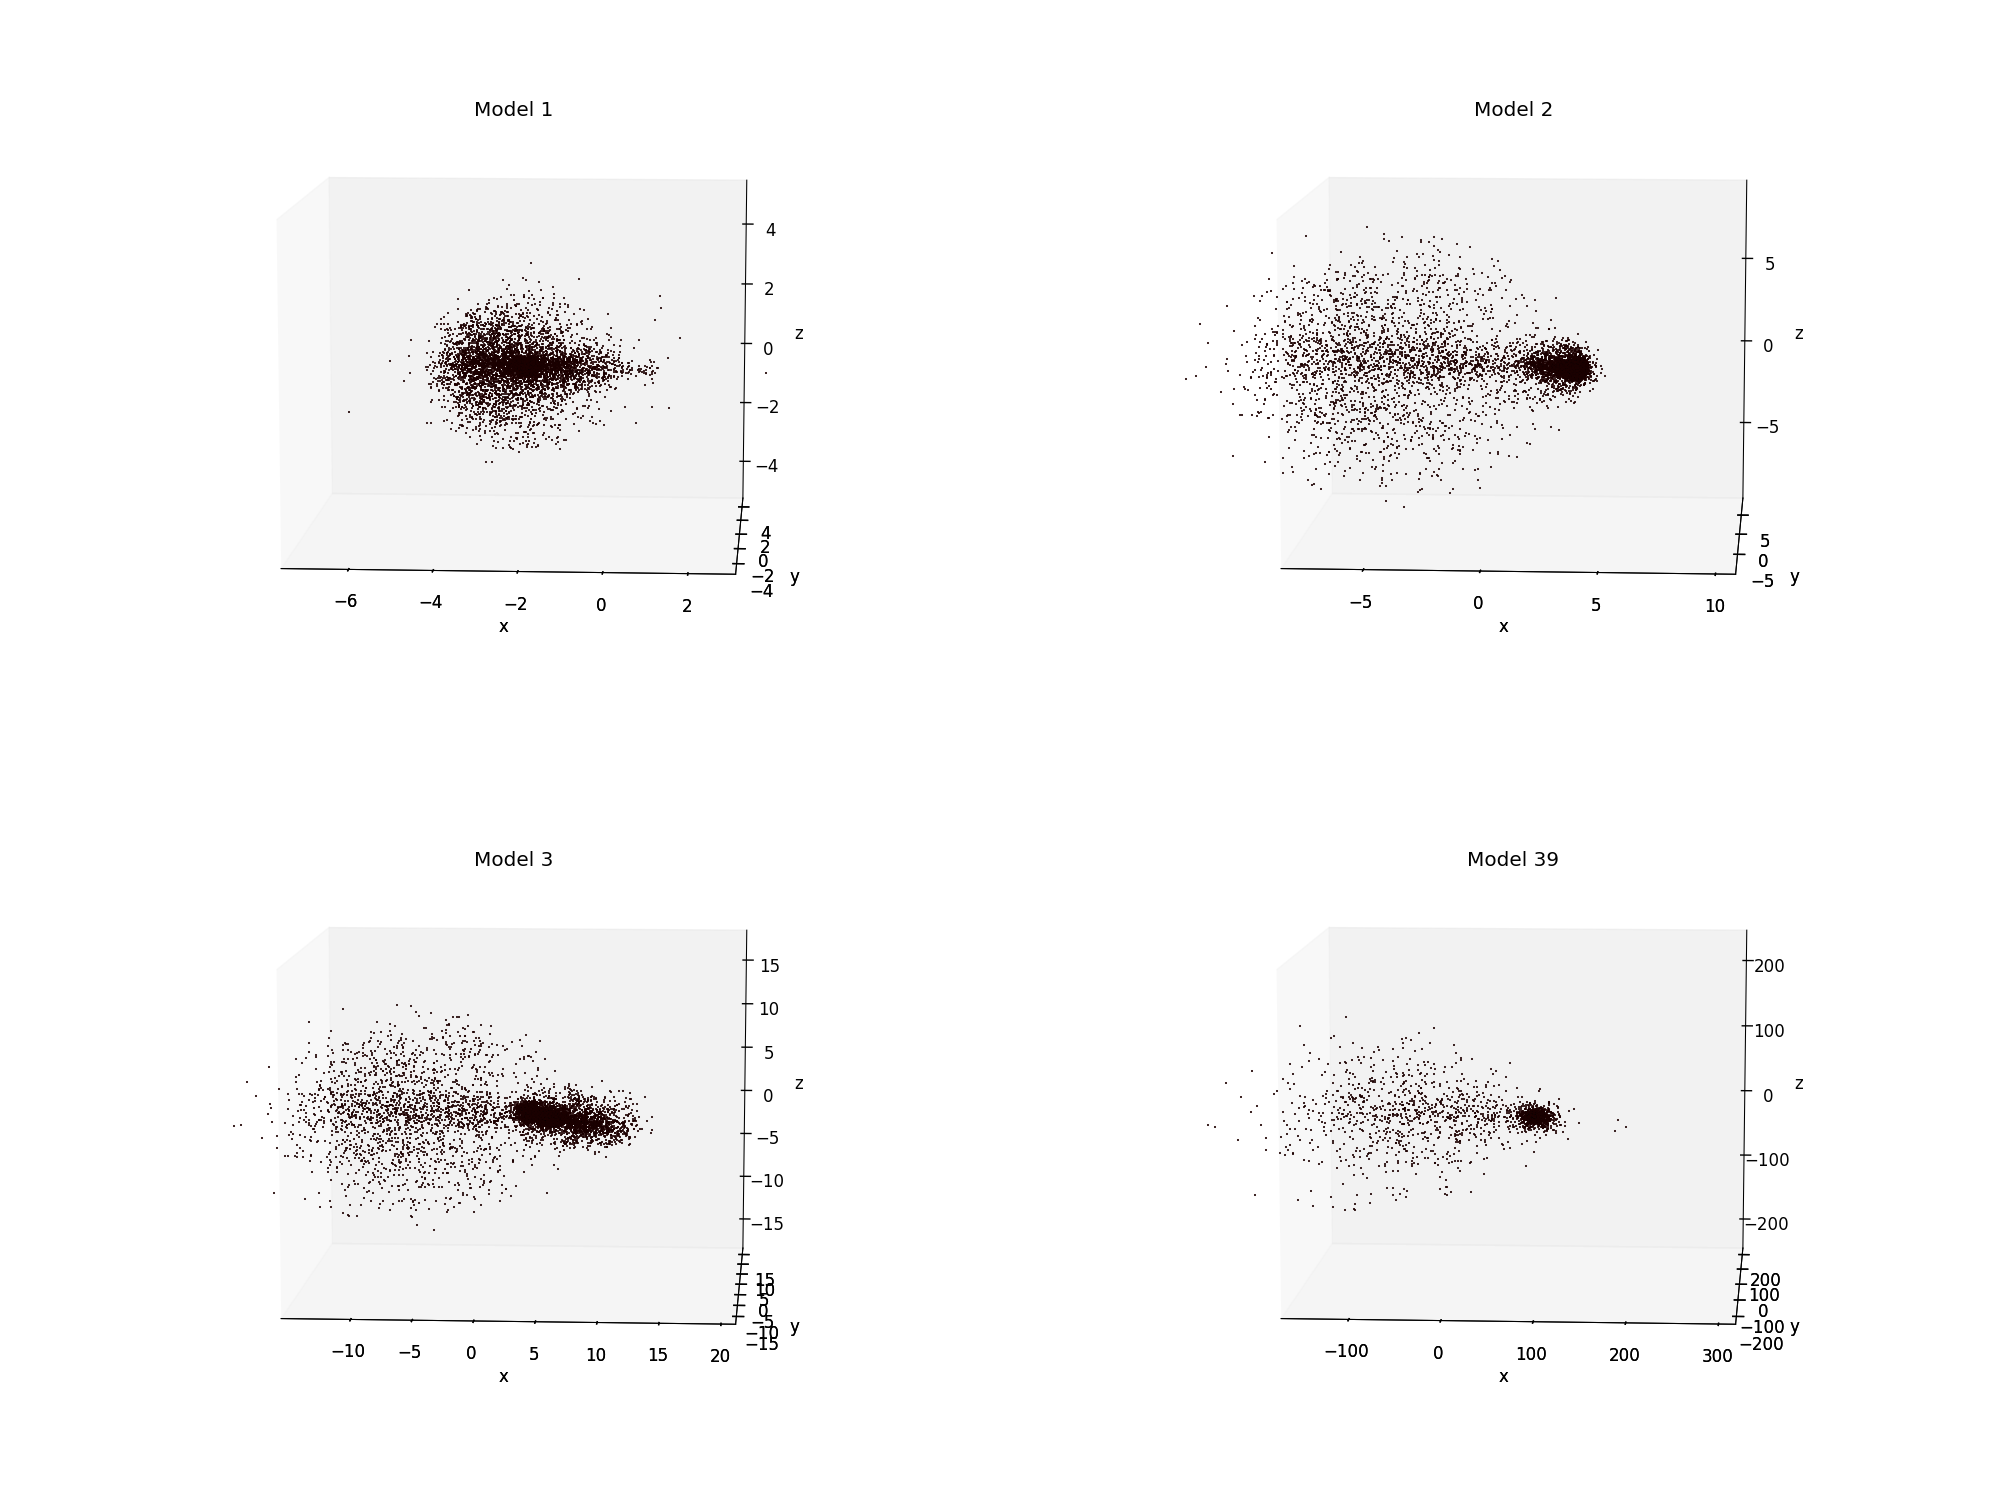
\includegraphics[scale=0.2]{sep590deg-2oy.png}
 \caption{\emph{ ángulo = 90 grados, el objeto esférico visto en la dirección oy(solo parte luminosa) modelo 1,2,3,39 }}
\end{figure}

\begin{figure}[!ht]
 \centering
 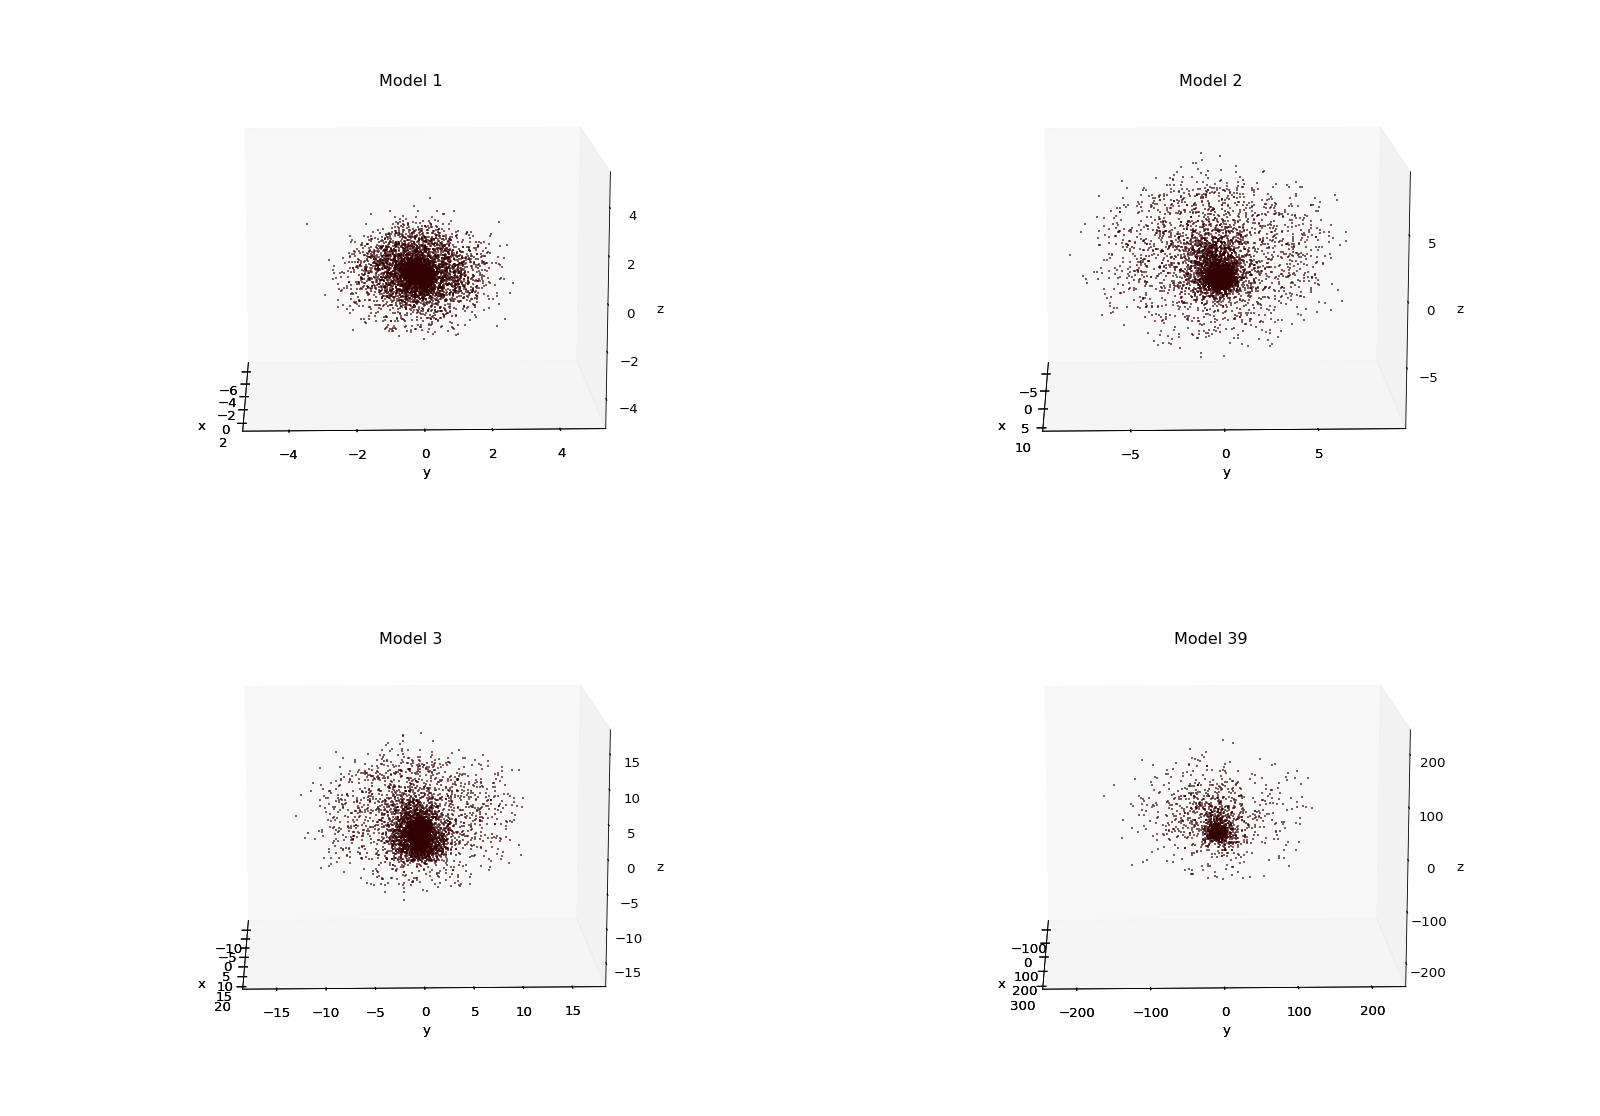
\includegraphics[scale=0.2]{sep5-90deg-eox.png}
 \caption{\emph{ ángulo = 90 grados, el objeto esférico visto en la dirección ox(solo parte luminosa) modelo 1,2,3,39 }}
\end{figure}

\begin{figure}[!ht]
 \centering
 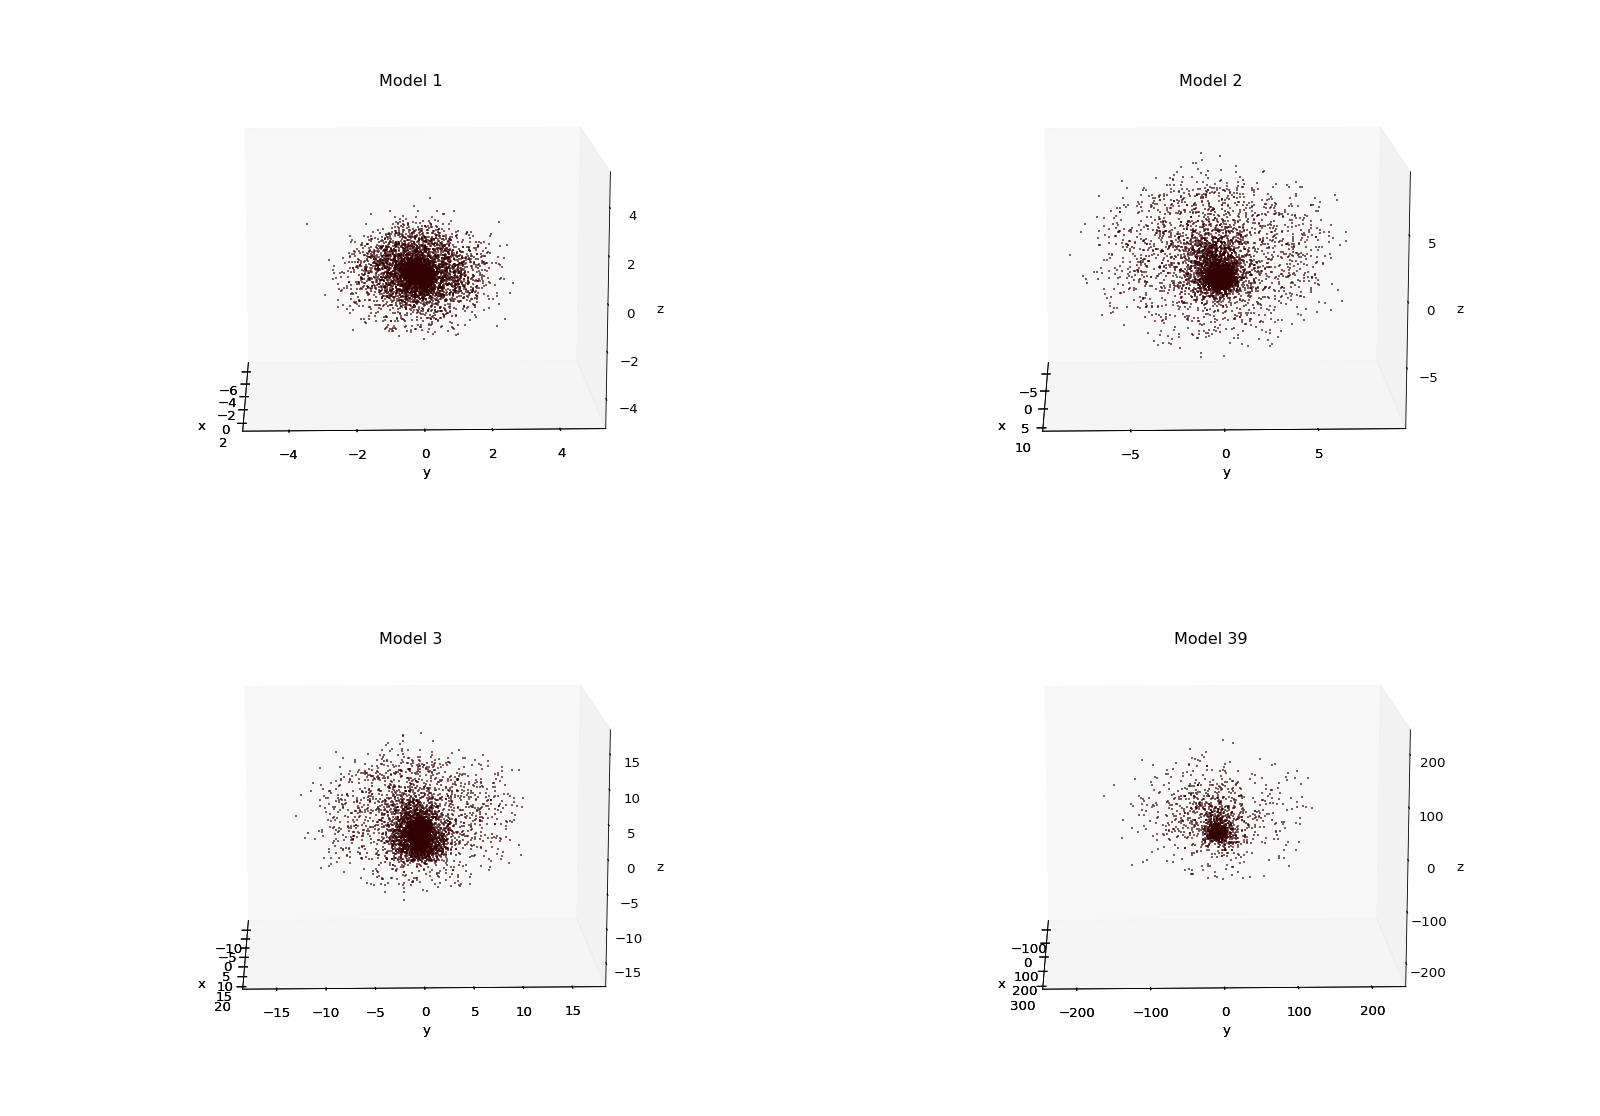
\includegraphics[scale=0.2]{sep590deg-2ox.png}
 \caption{\emph{ ángulo = 90 grados, el objeto esférico visto en la dirección ox(solo parte luminosa) modelo 1,2,3,39 }}
\end{figure}

\begin{figure}[!ht]
 \centering
 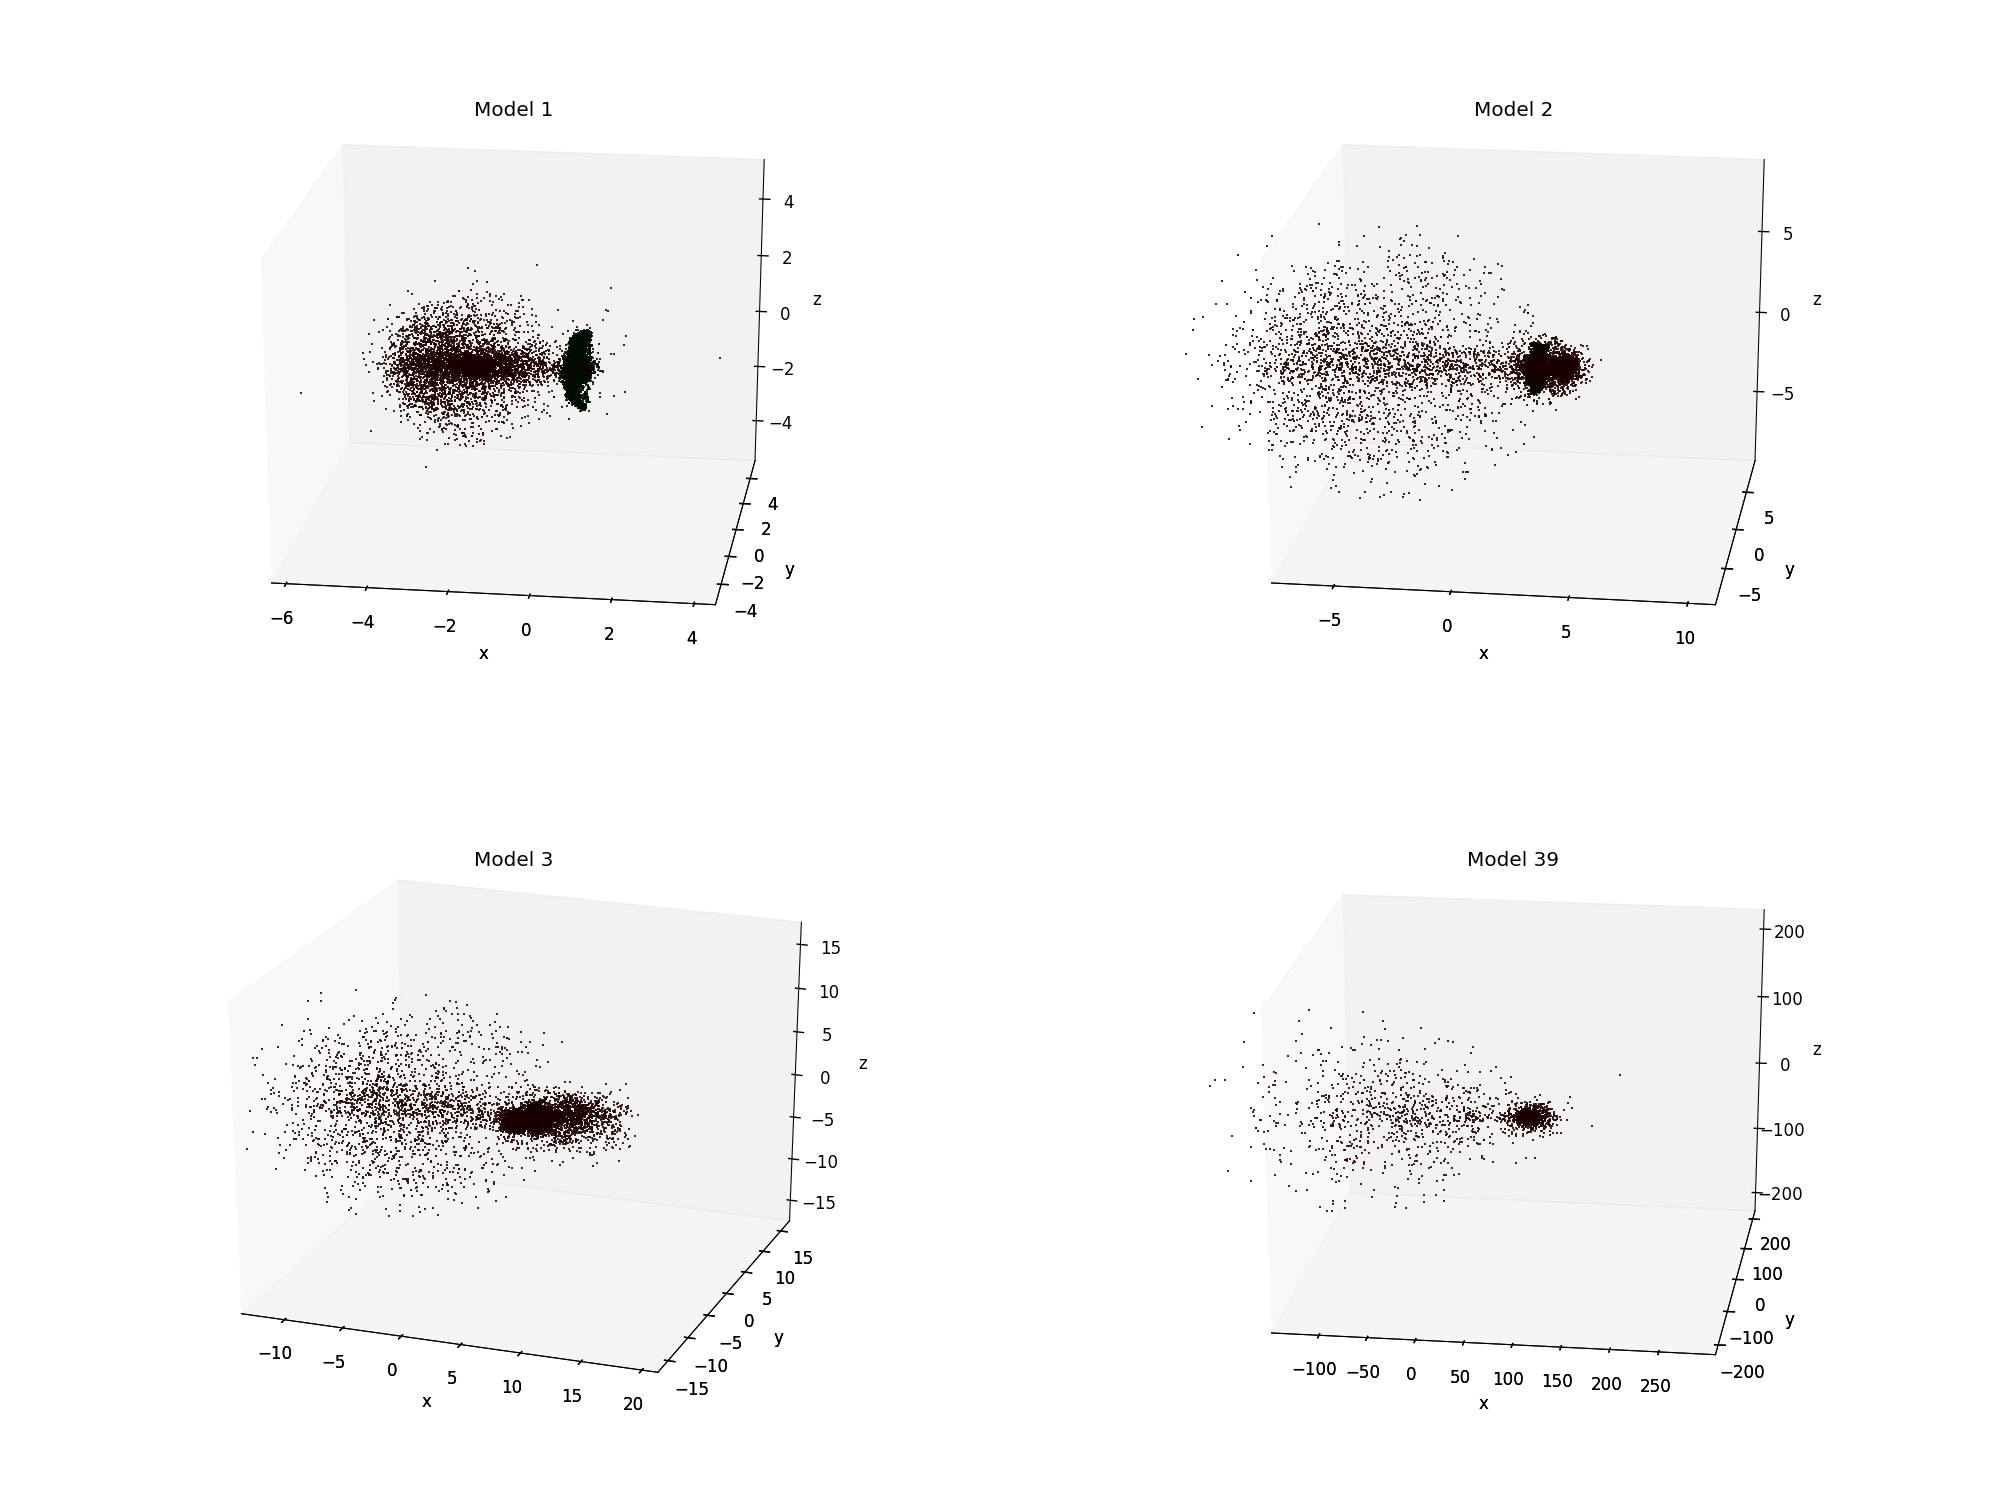
\includegraphics[scale=0.2]{270deg_m_sep5.png}
 \caption{\emph{ ángulo = 270 grados, los 2 objetos(solo parte luminosa) modelo 1,2,3,39 }}
\end{figure}

\begin{figure}[!ht]
 \centering
 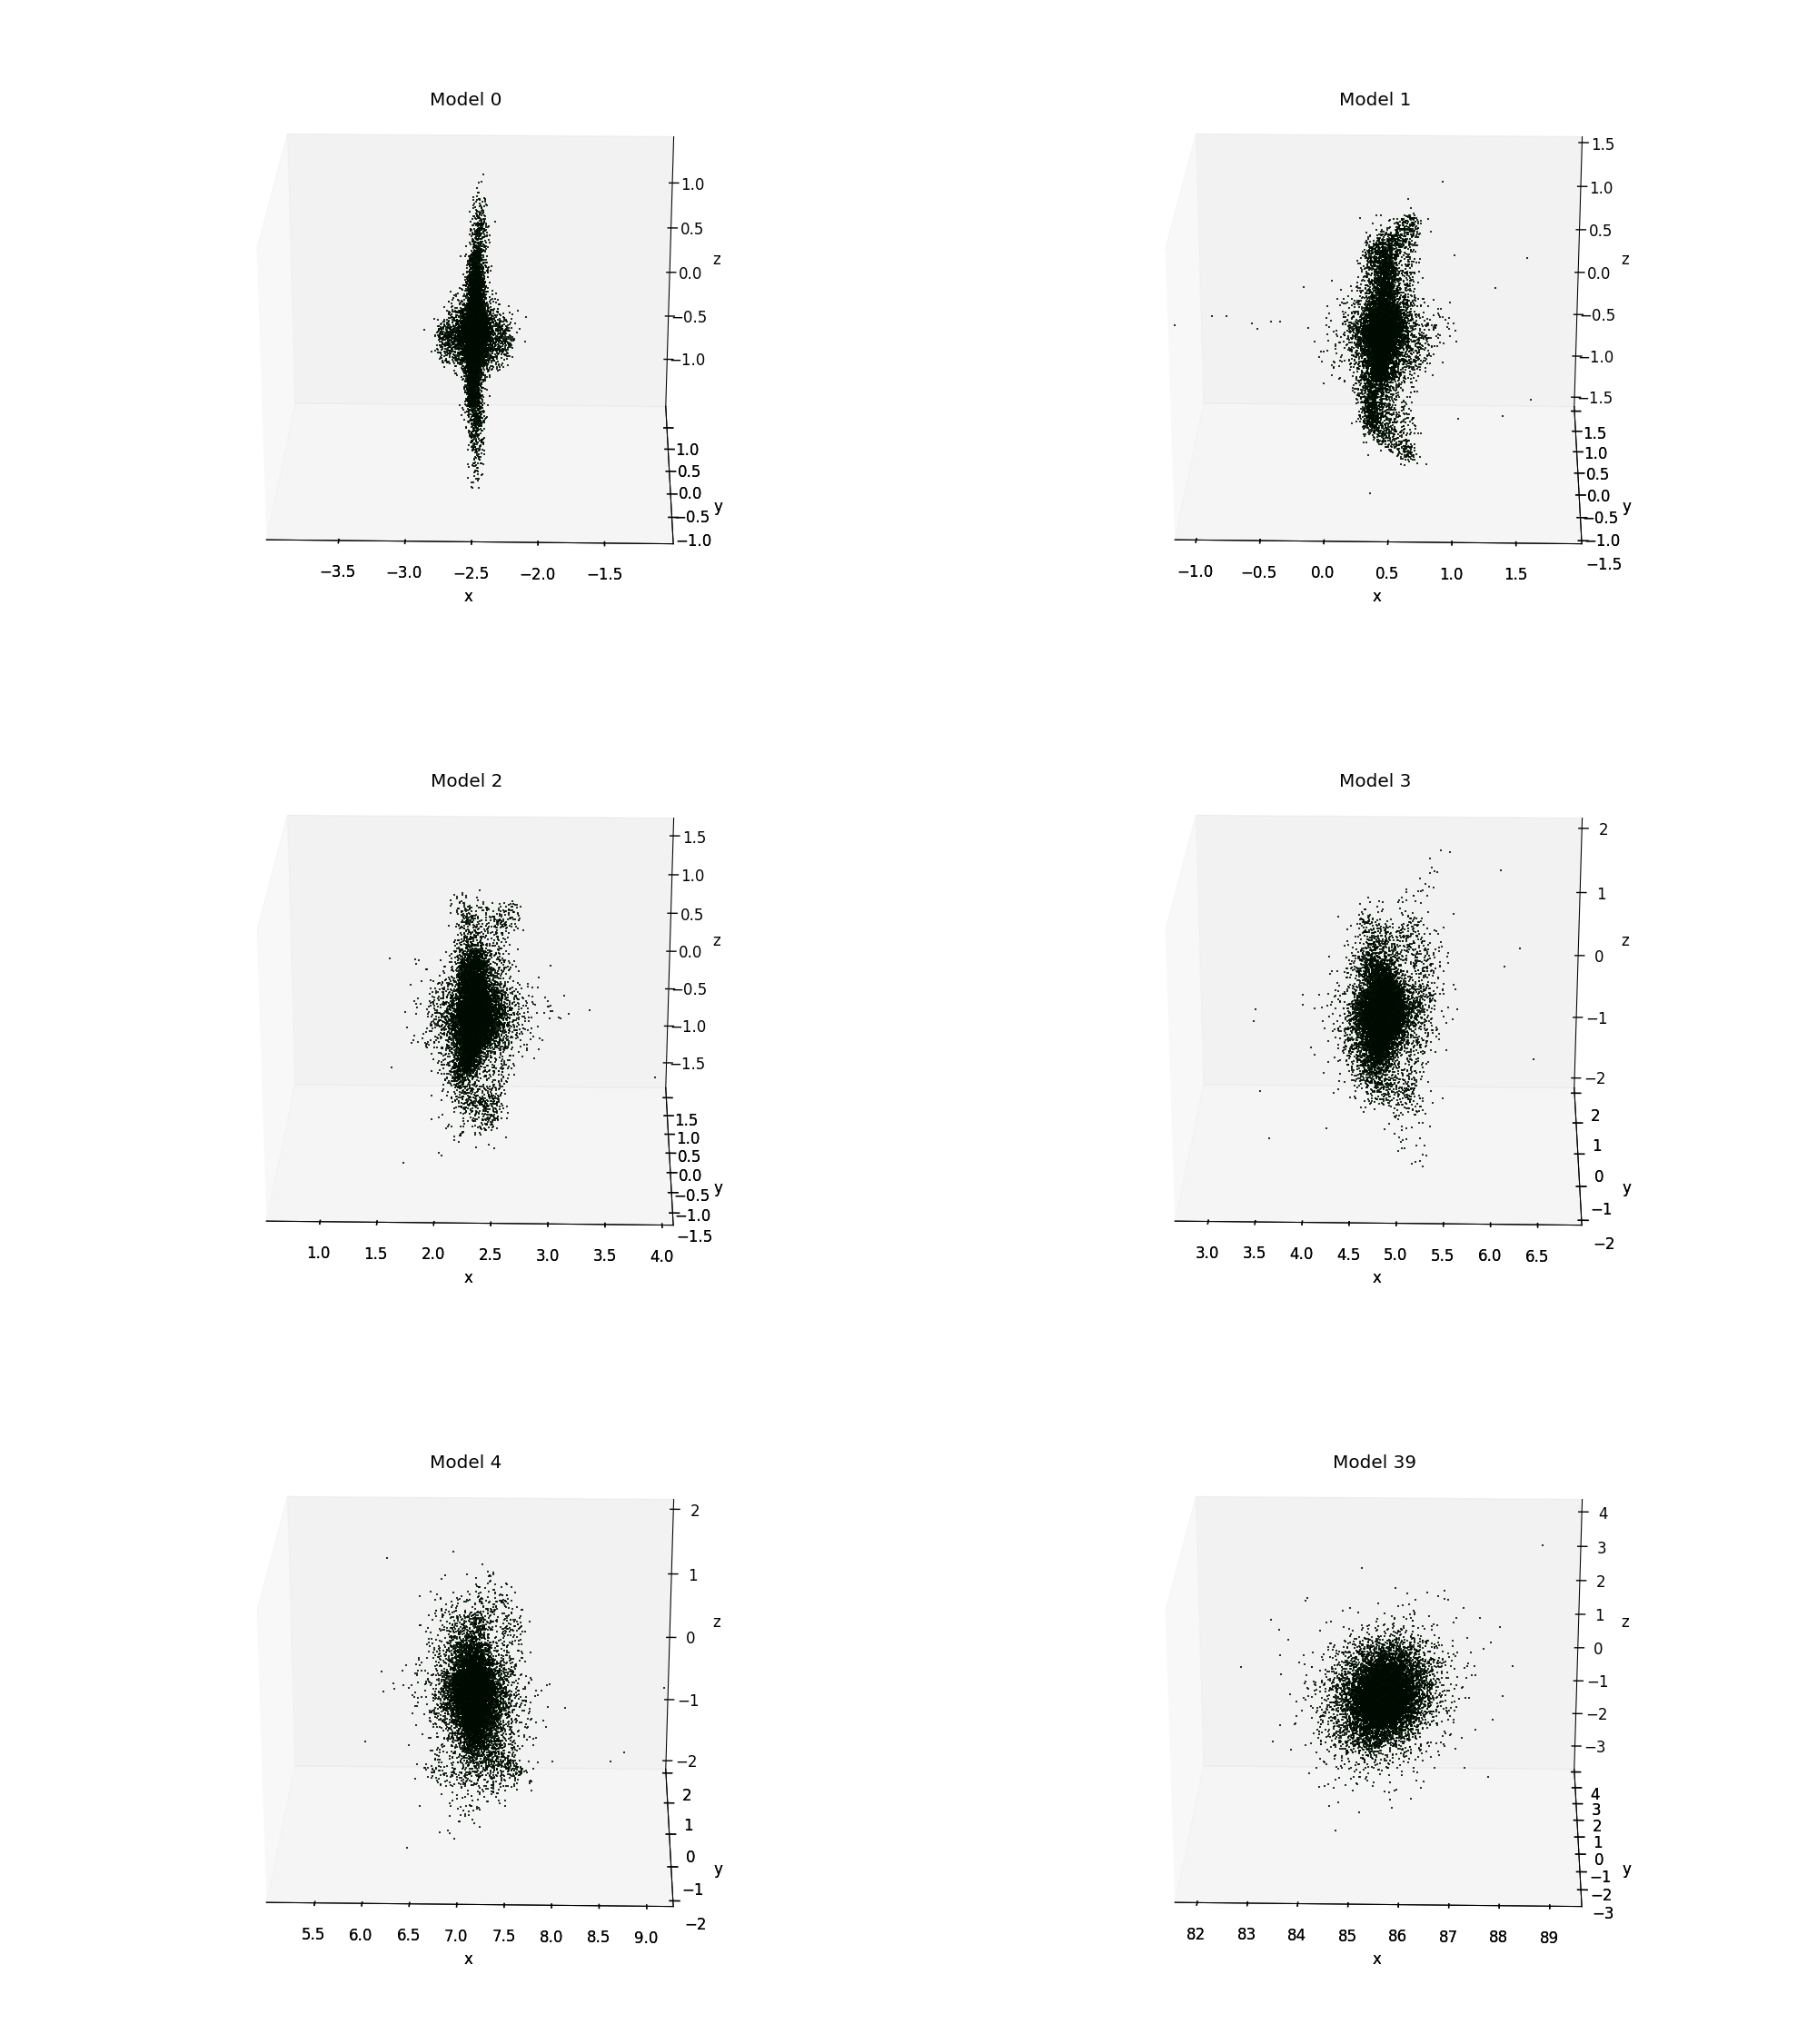
\includegraphics[scale=0.2]{270deg-m-c2y.png}
 \caption{\emph{ ángulo = 270 grados, el objeto con disco visto en la dirección oy(solo parte luminosa) modelo 0,1,2,3,4,39 }}
\end{figure}

\begin{figure}[!ht]
 \centering
 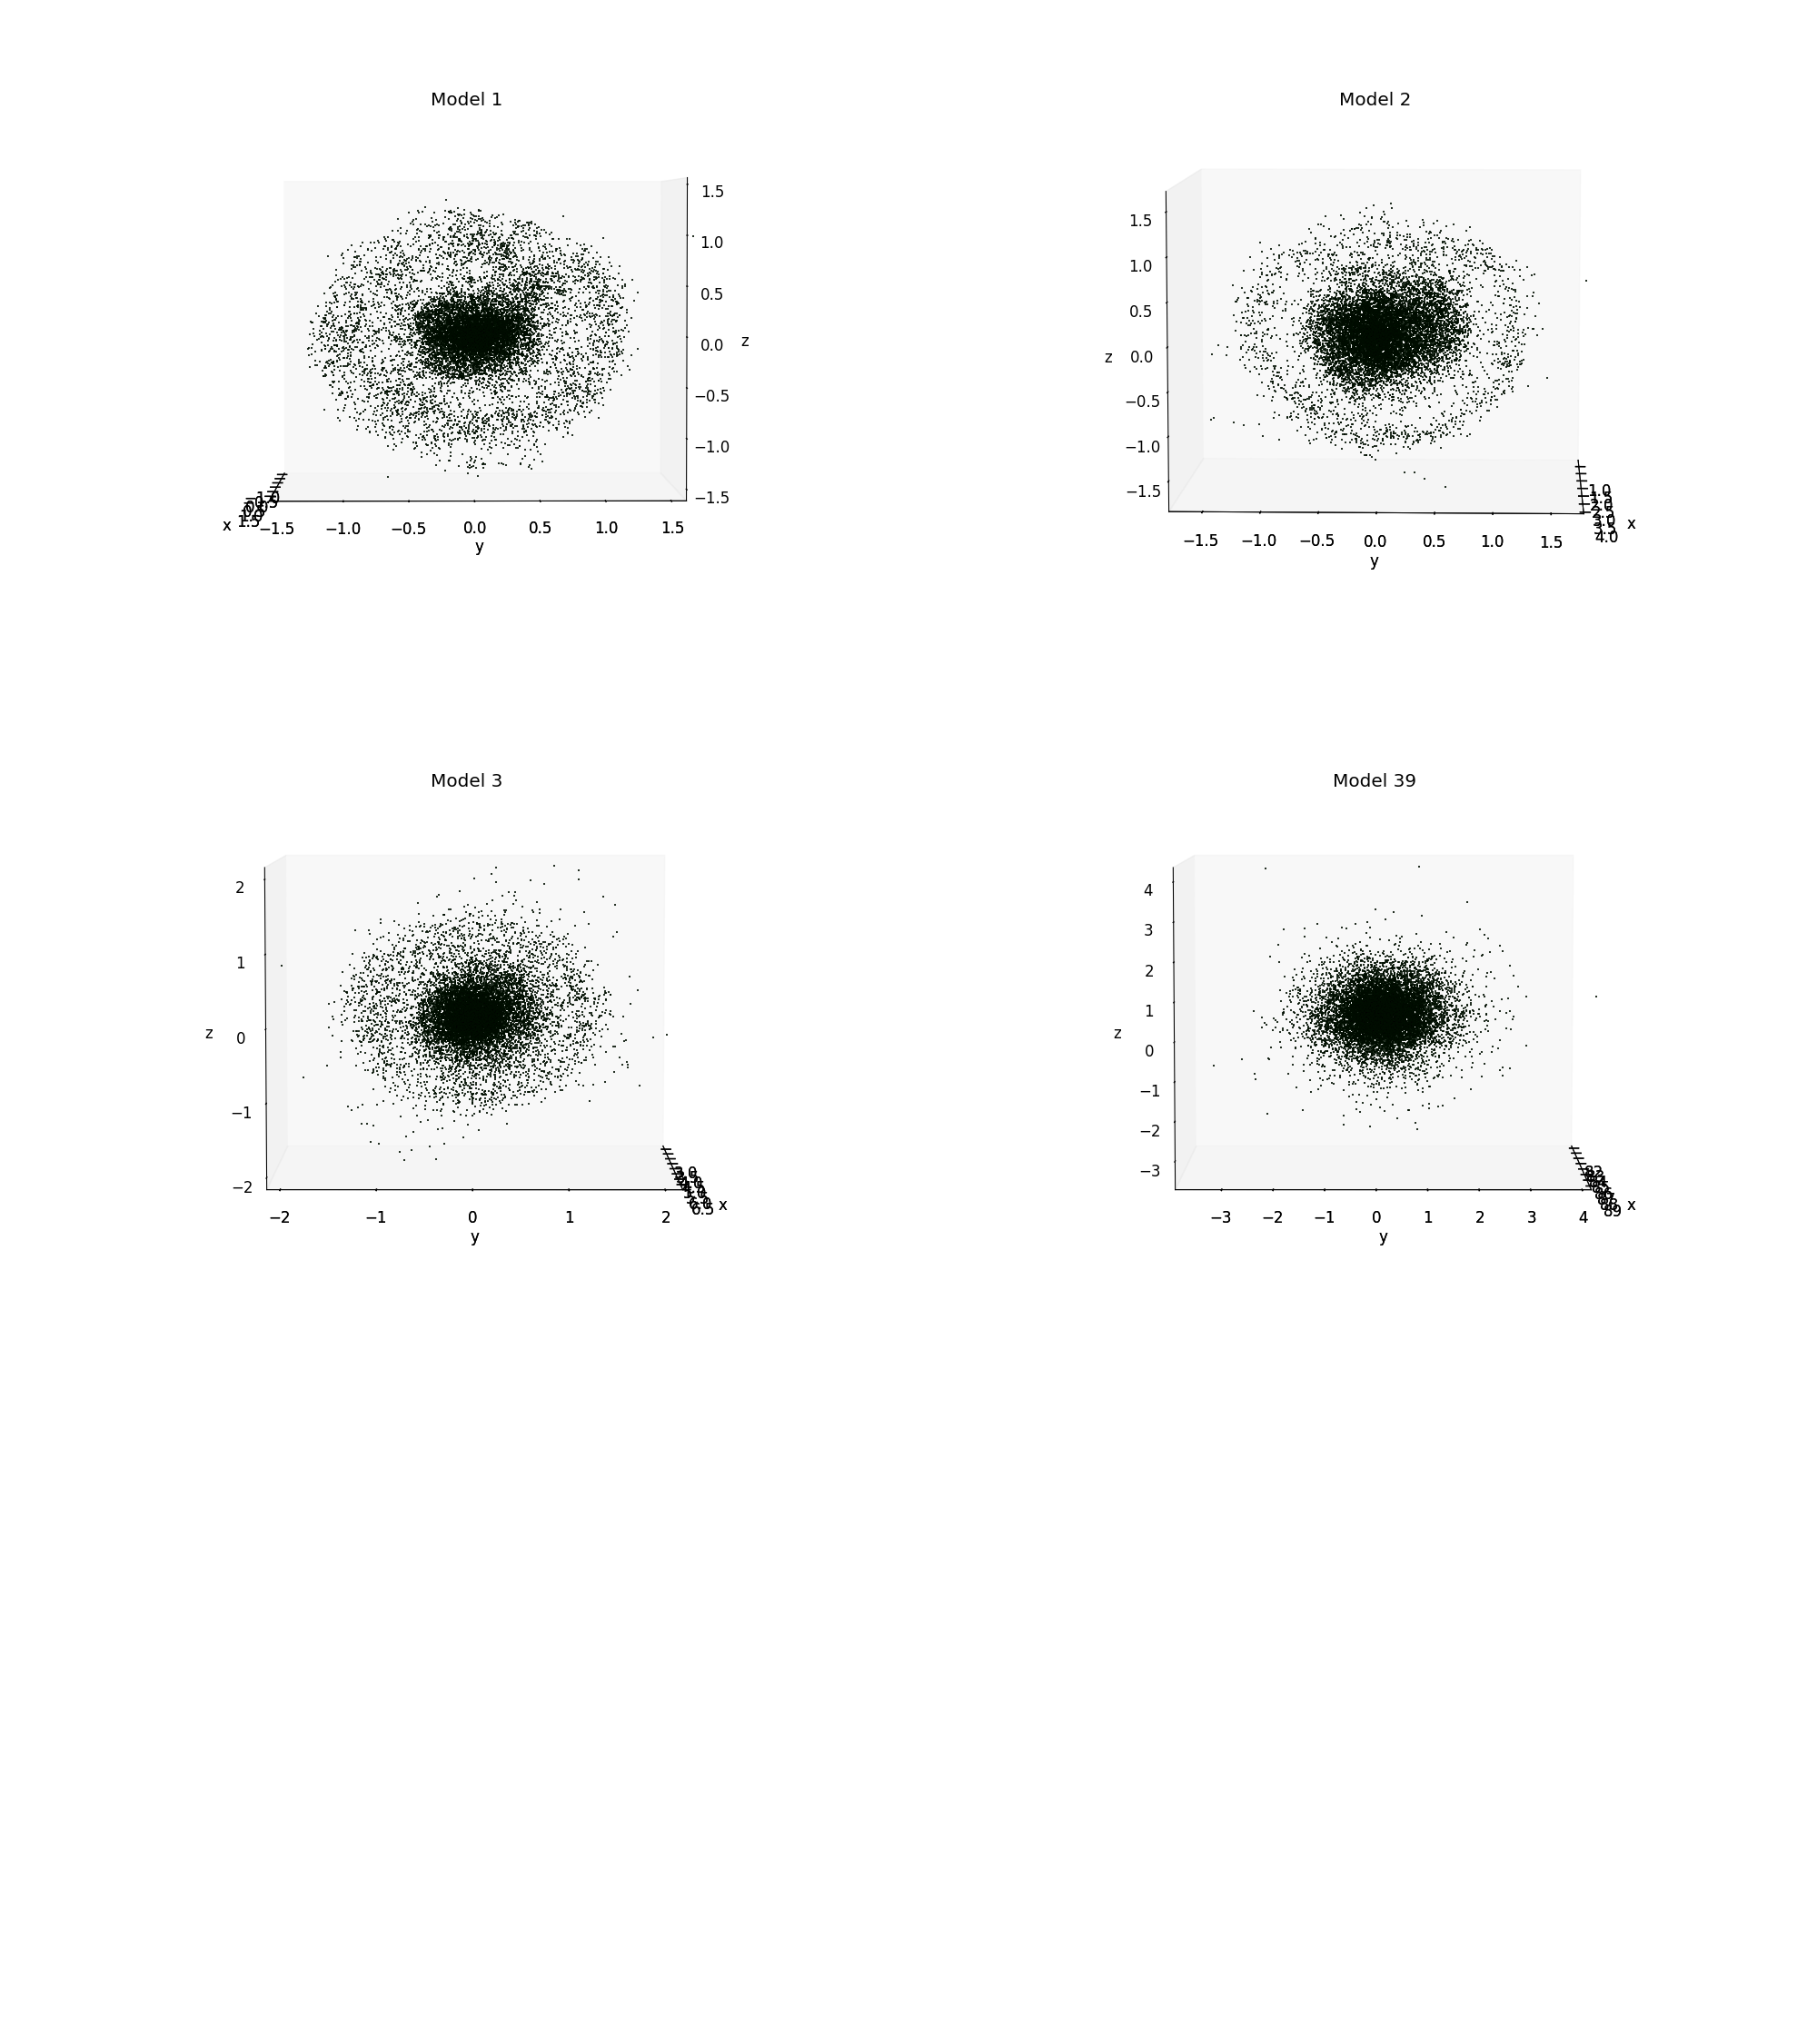
\includegraphics[scale=0.2]{270deg-m-c2.png}
 \caption{\emph{ ángulo = 270 grados, el objeto con disco visto en la dirección ox(solo parte luminosa) modelo 1,2,3,39 }}
\end{figure}

\begin{figure}[!ht]
 \centering
 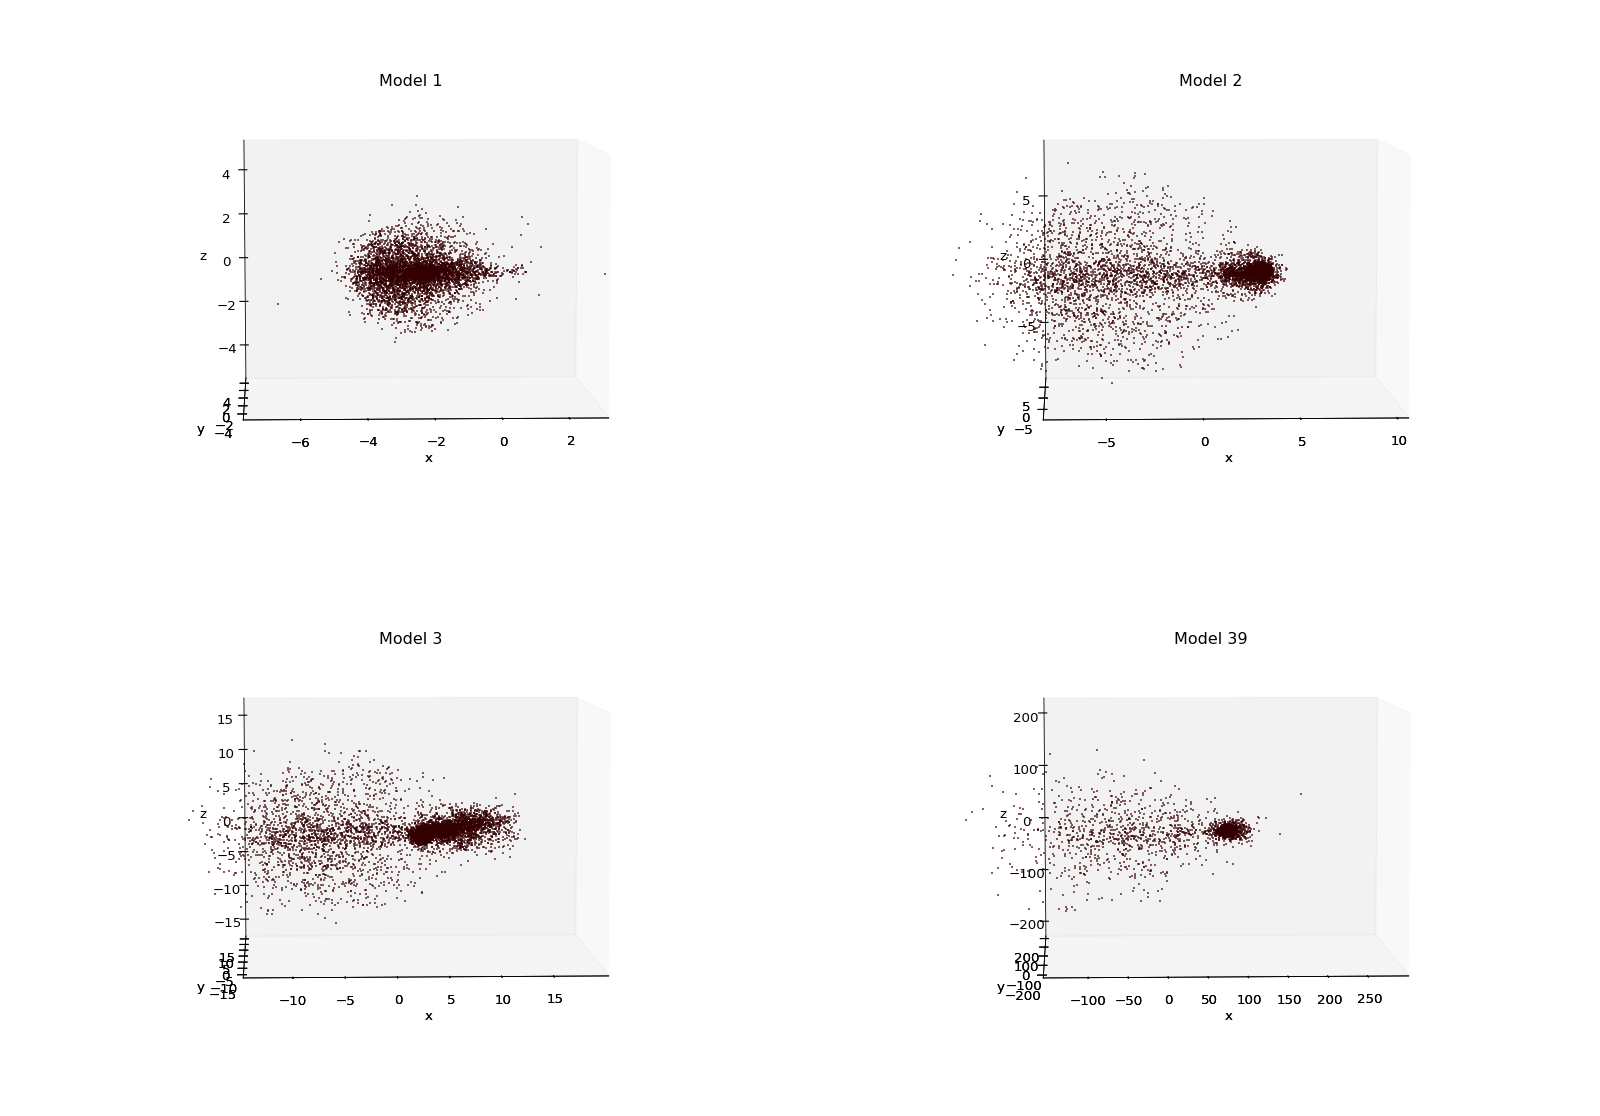
\includegraphics[scale=0.2]{sep5-270deg-eoy.png}
 \caption{\emph{ ángulo = 270 grados, el objeto esférico visto en la dirección oy(solo parte luminosa) modelo 1,2,3,39 }}
\end{figure}

\begin{figure}[!ht]
 \centering
 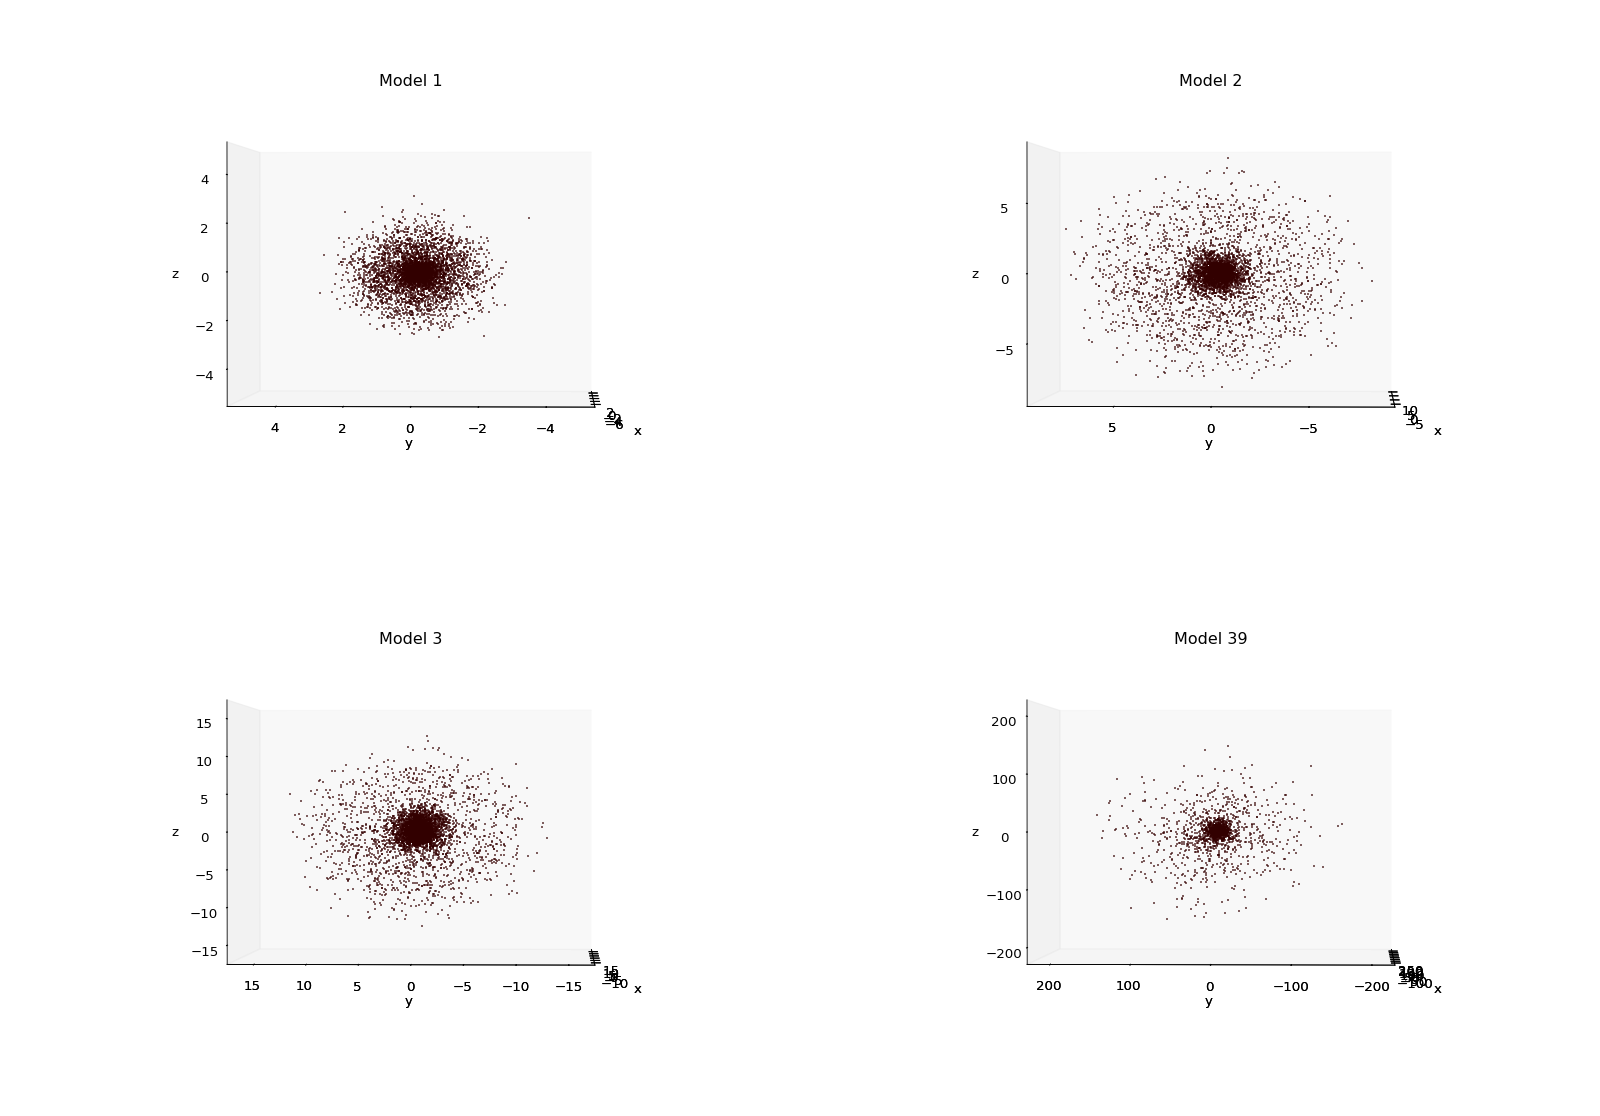
\includegraphics[scale=0.2]{sep5-270deg-eox.png}
 \caption{\emph{ ángulo = 270 grados, el objeto esférico visto en la dirección ox(solo parte luminosa) modelo 1,2,3,39 }}
\end{figure}

\begin{figure}[!ht]
 \centering
 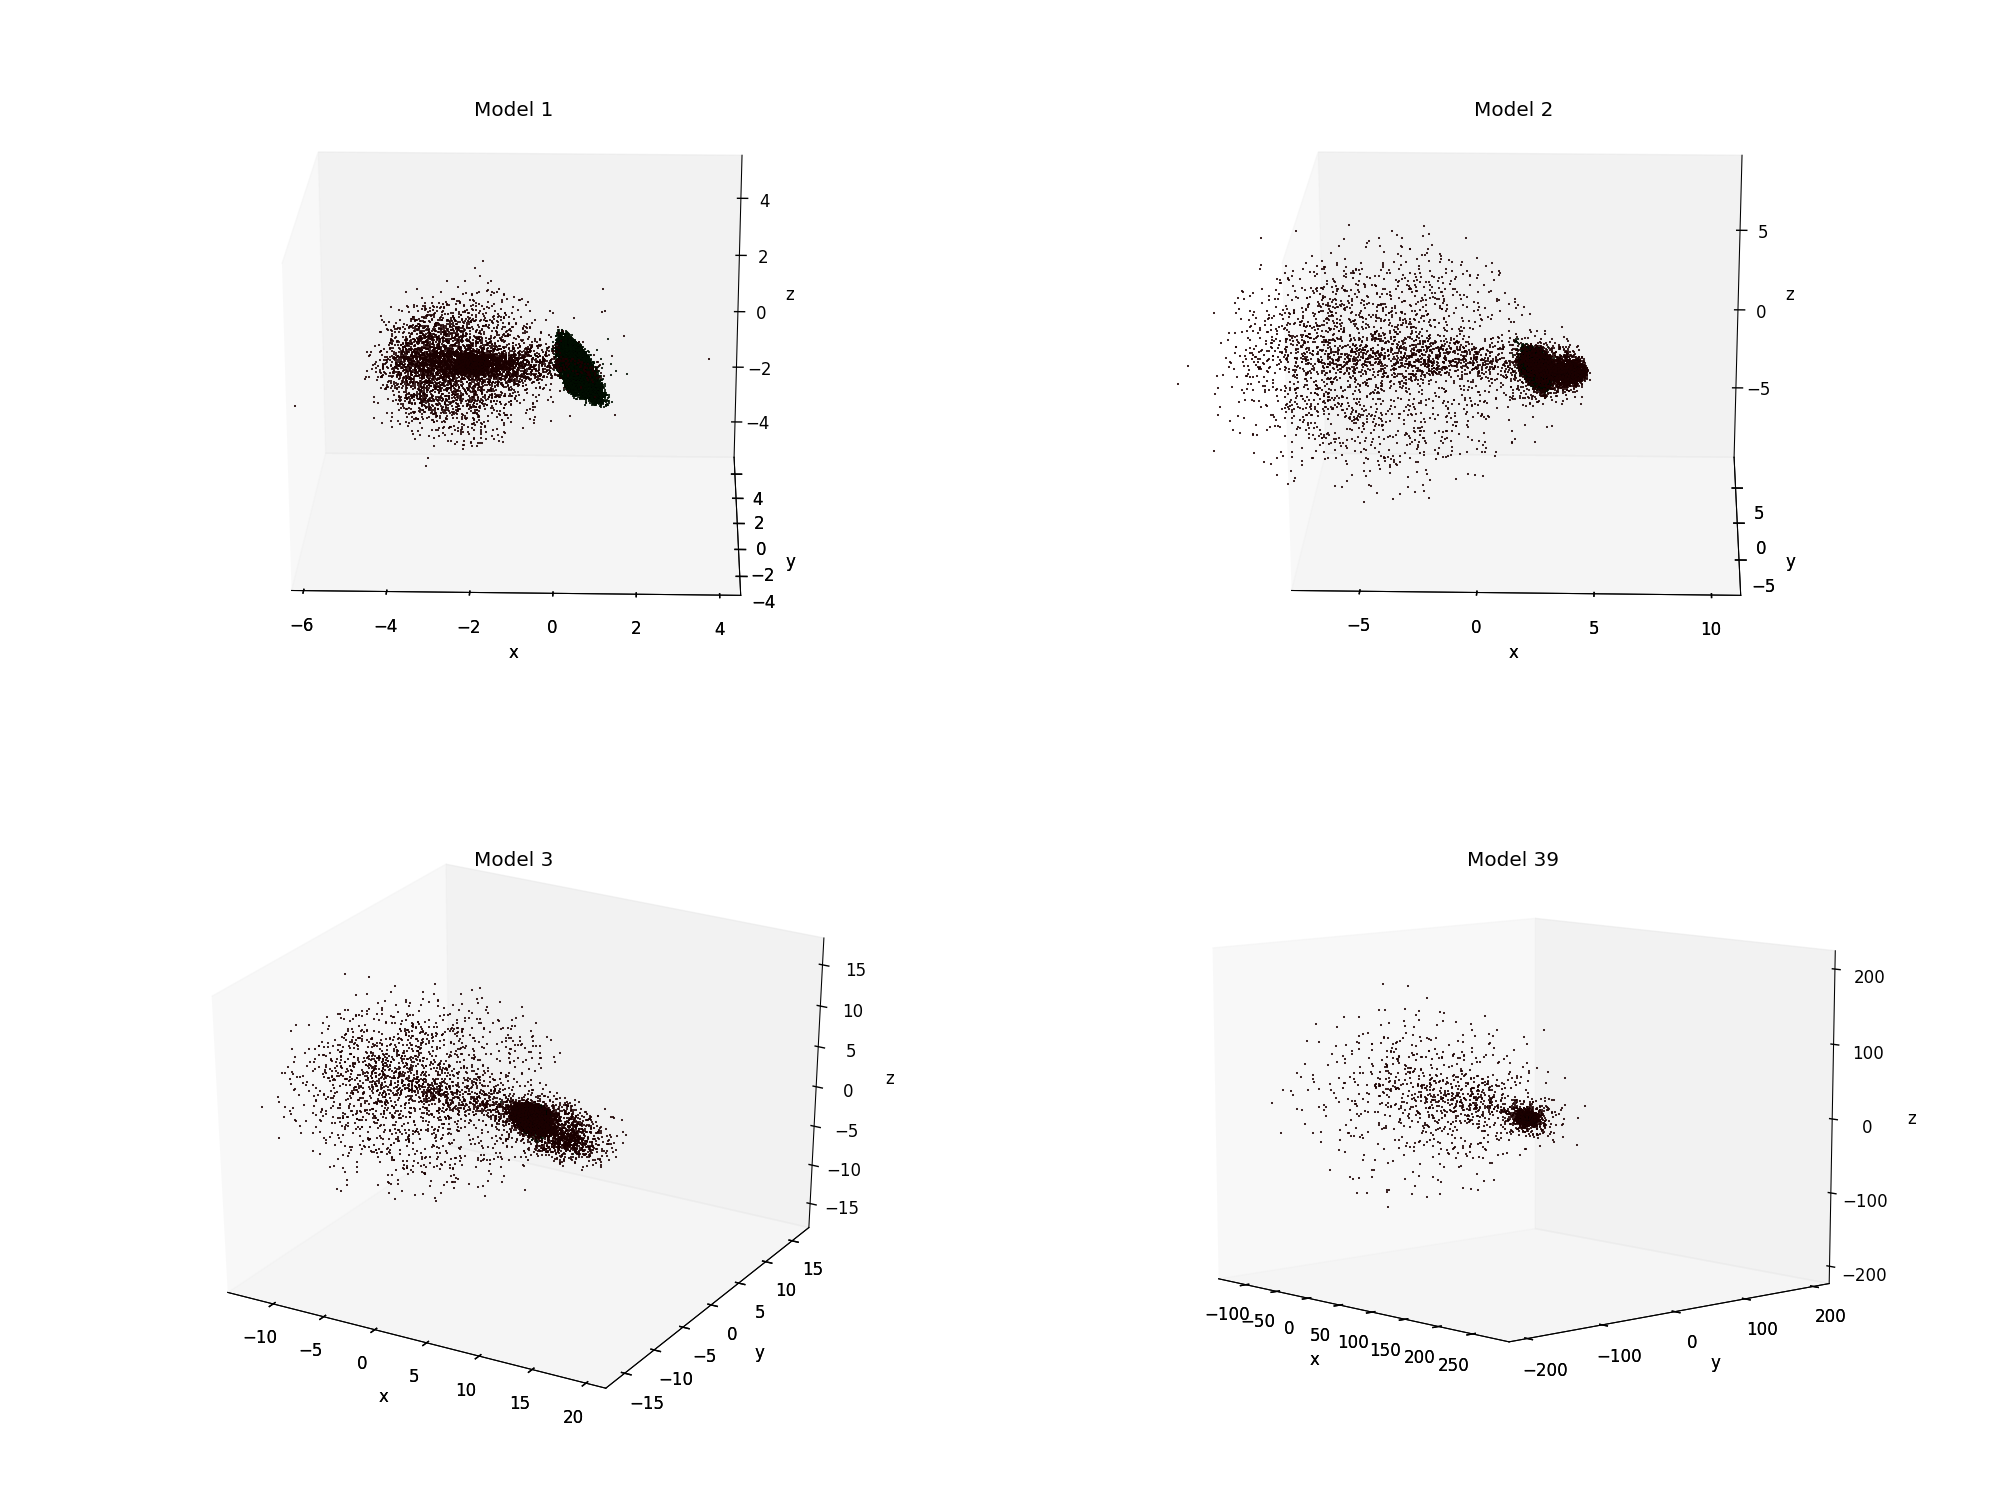
\includegraphics[scale=0.2]{60deg-m.png}
 \caption{\emph{ ángulo = 60 grados, los 2 objetos(solo parte luminosa) modelo 1,2,3,39 }}
\end{figure}

\begin{figure}[!ht]
 \centering
 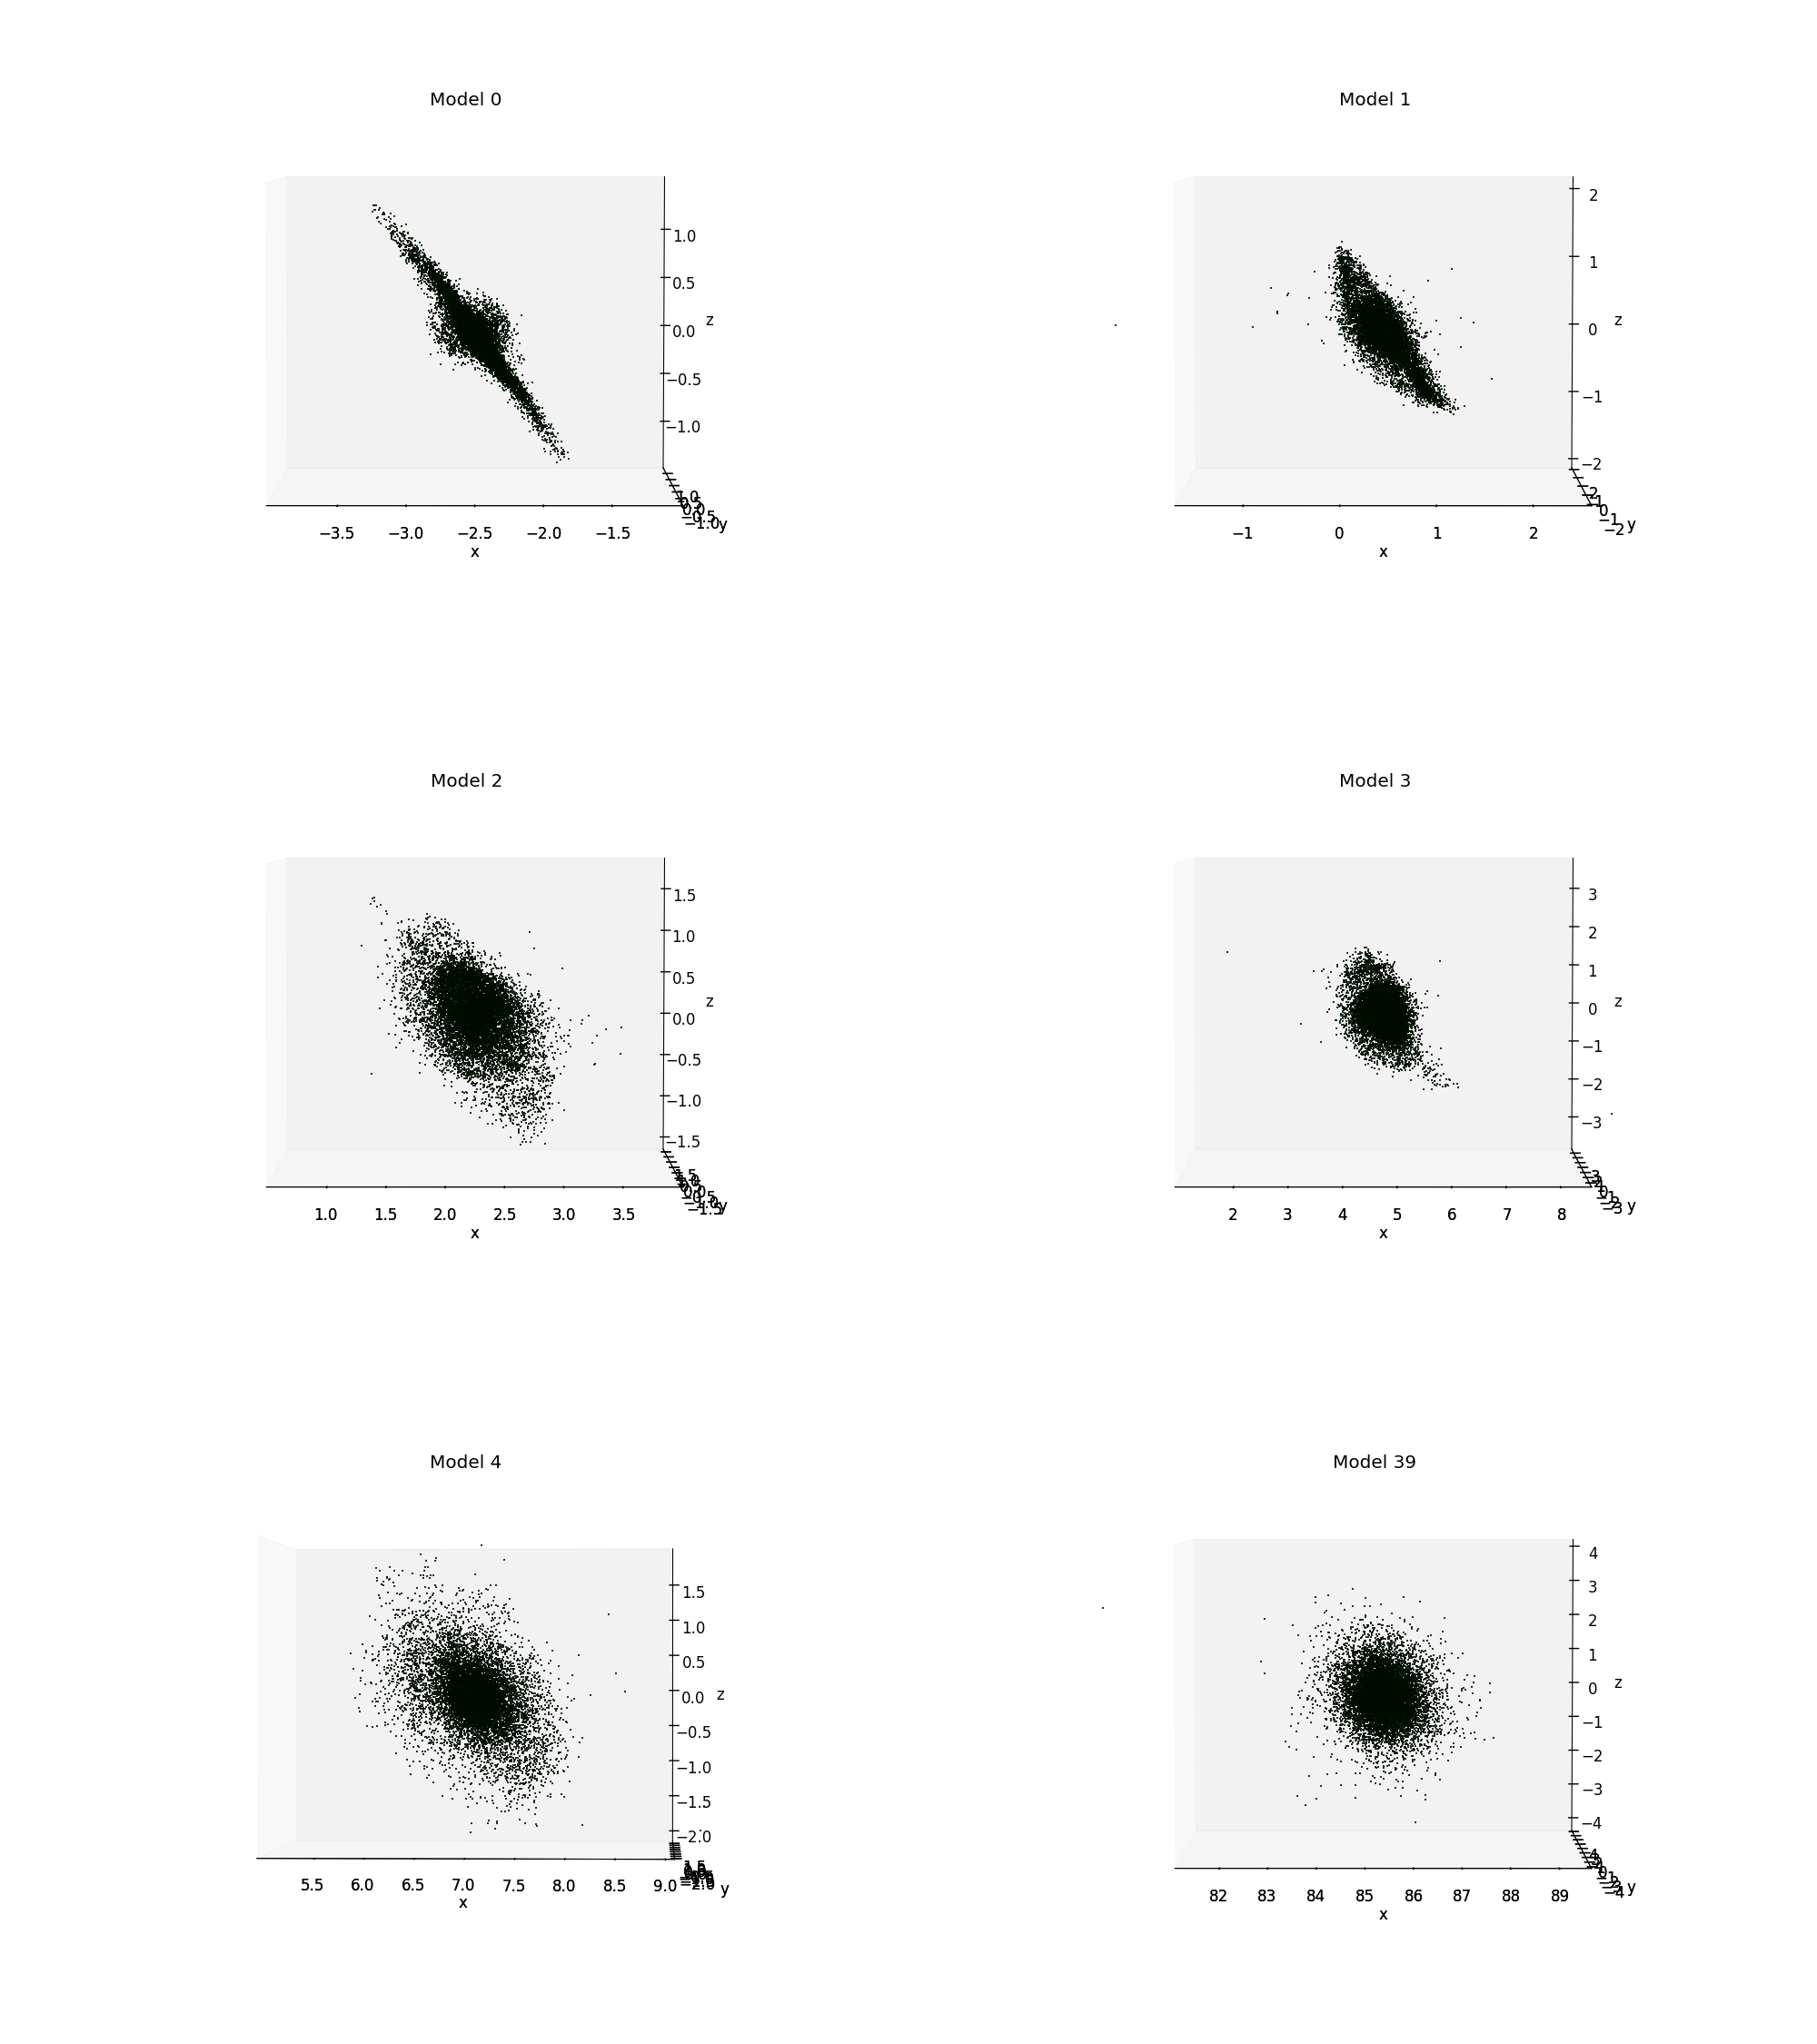
\includegraphics[scale=0.2]{60deg-m-c2y.png}
 \caption{\emph{ ángulo = 60 grados, el objeto con disco visto en la dirección oy(solo parte luminosa) modelo 0,1,2,3,4,39 }}
\end{figure}

\begin{figure}[!ht]
 \centering
 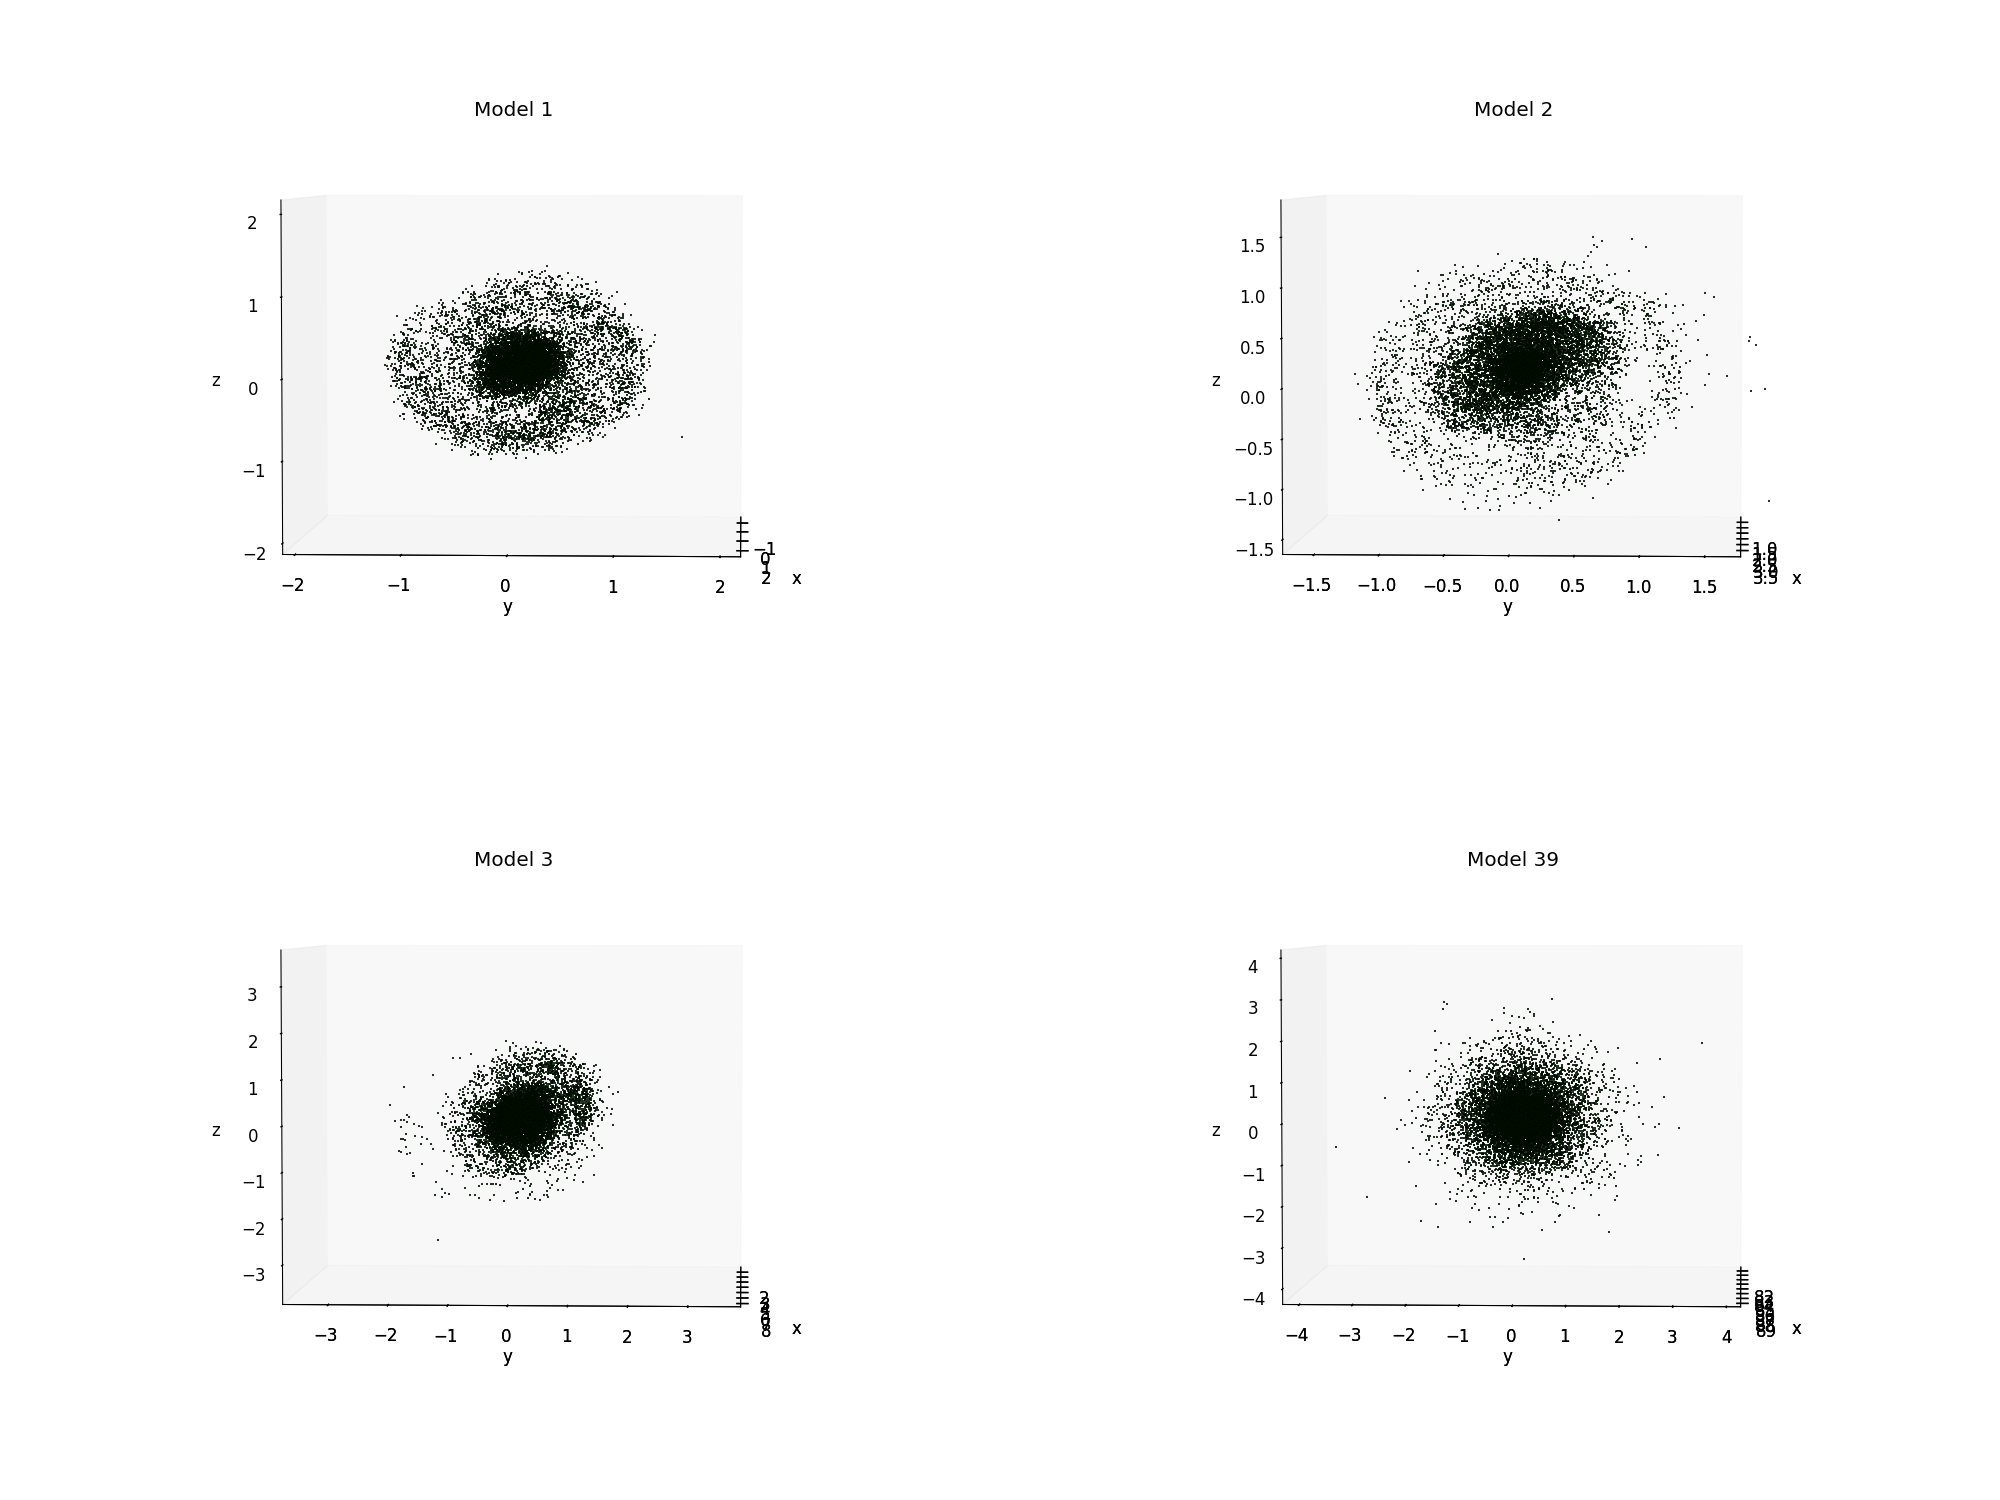
\includegraphics[scale=0.2]{60deg-m-c2.png}
 \caption{\emph{ ángulo = 60 grados, el objeto con disco visto en la dirección ox(solo parte luminosa) modelo 1,2,3,39 }}
\end{figure}

\begin{figure}[!ht]
 \centering
 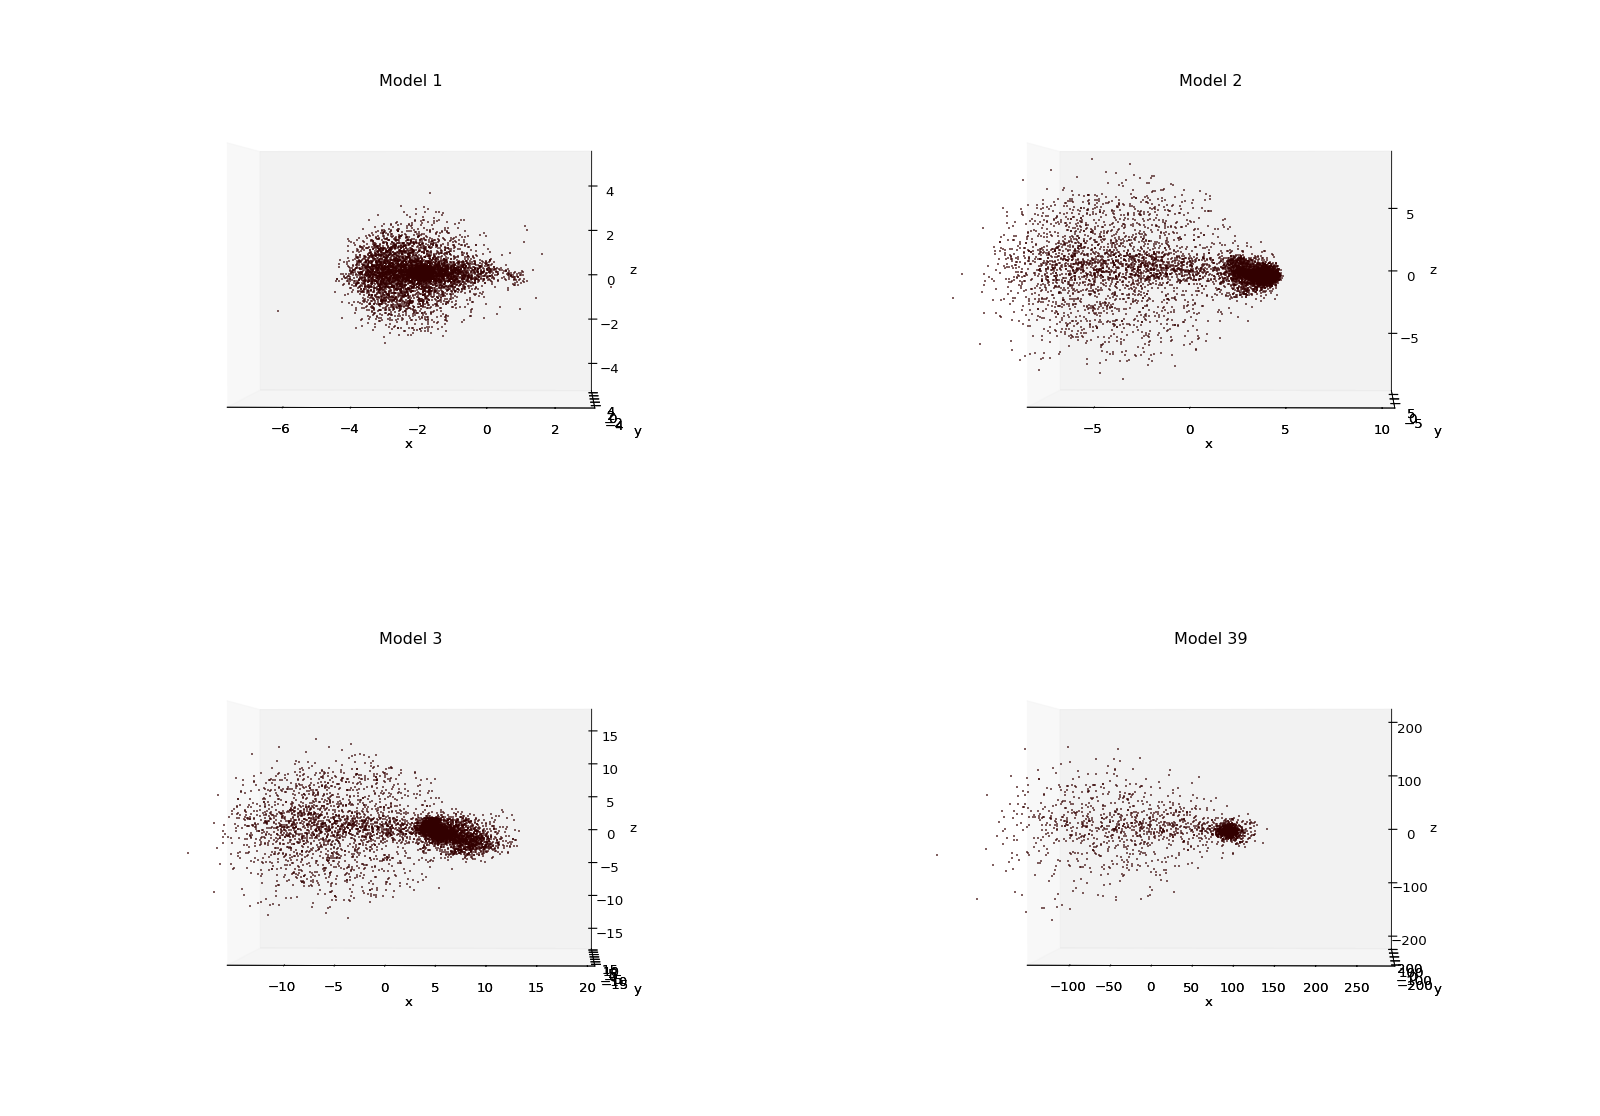
\includegraphics[scale=0.2]{sep5-60deg-eoy.png}
 \caption{\emph{ ángulo = 60 grados, el objeto esférico visto en la dirección oy(solo parte luminosa) modelo 1,2,3,39 }}
\end{figure}

\begin{figure}[!ht]
 \centering
 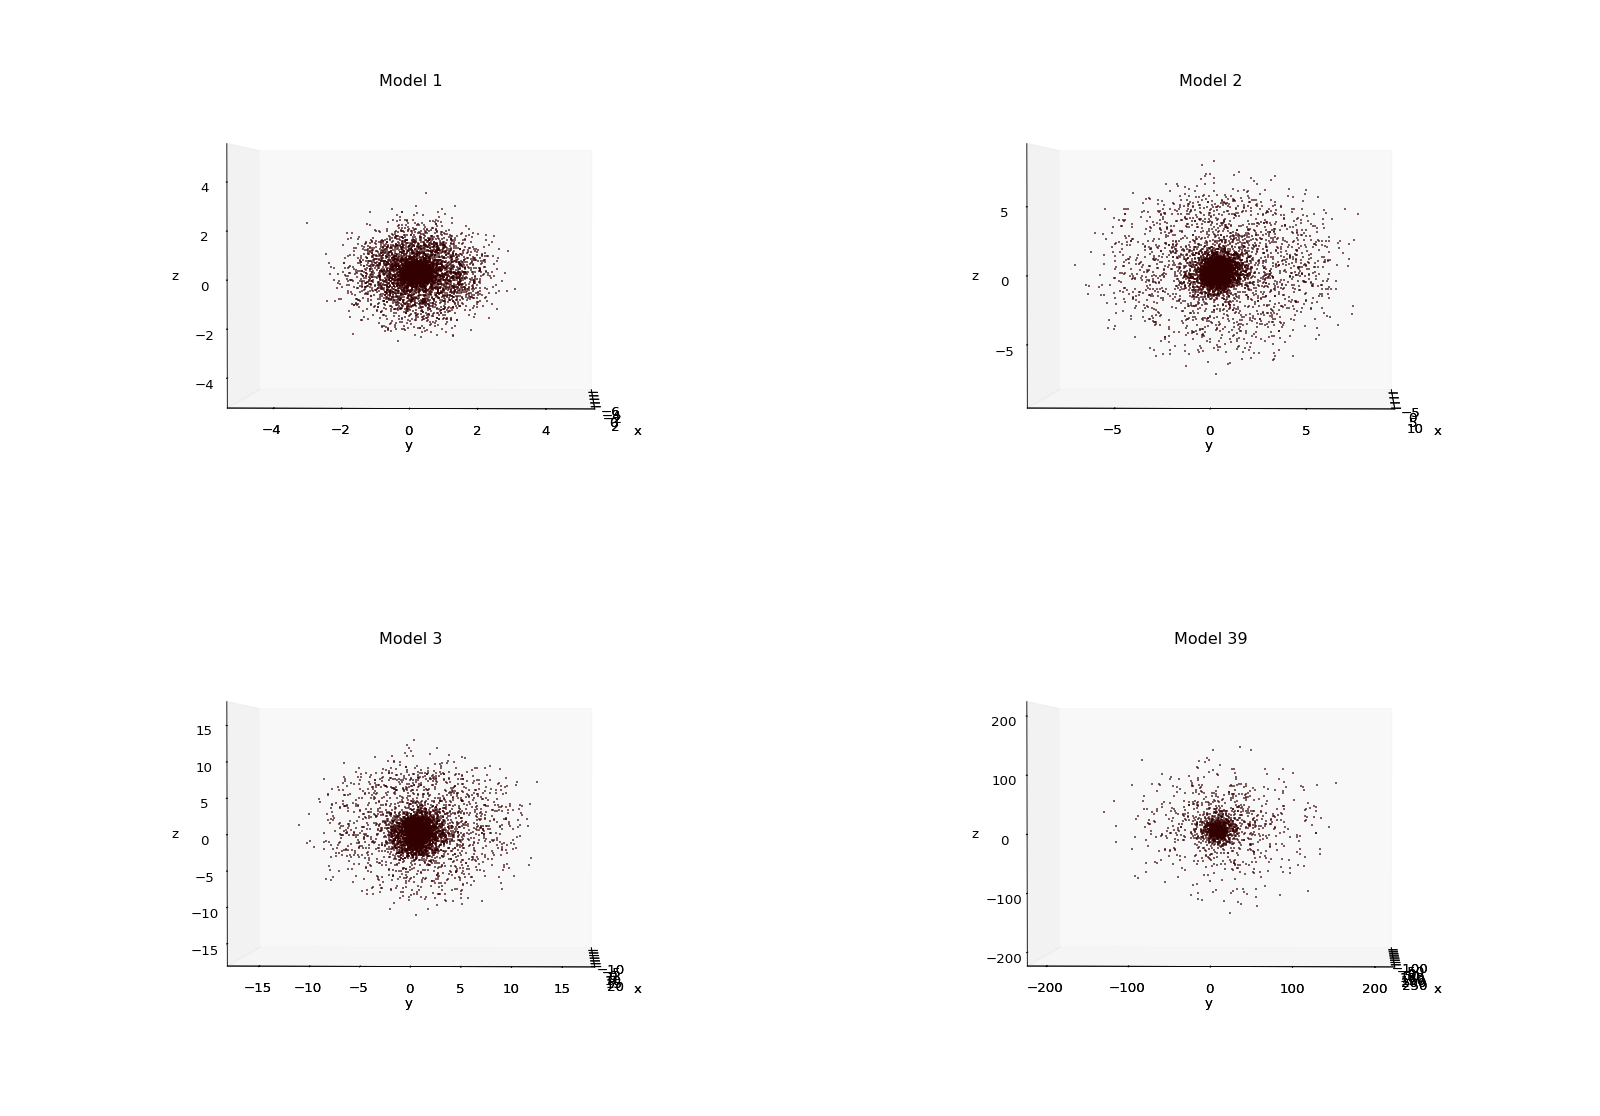
\includegraphics[scale=0.2]{sep5-60deg-eox.png}
 \caption{\emph{ ángulo = 60 grados, el objeto esférico visto en la dirección ox(solo parte luminosa) modelo 1,2,3,39 }}
\end{figure}

\begin{figure}[!ht]
 \centering
 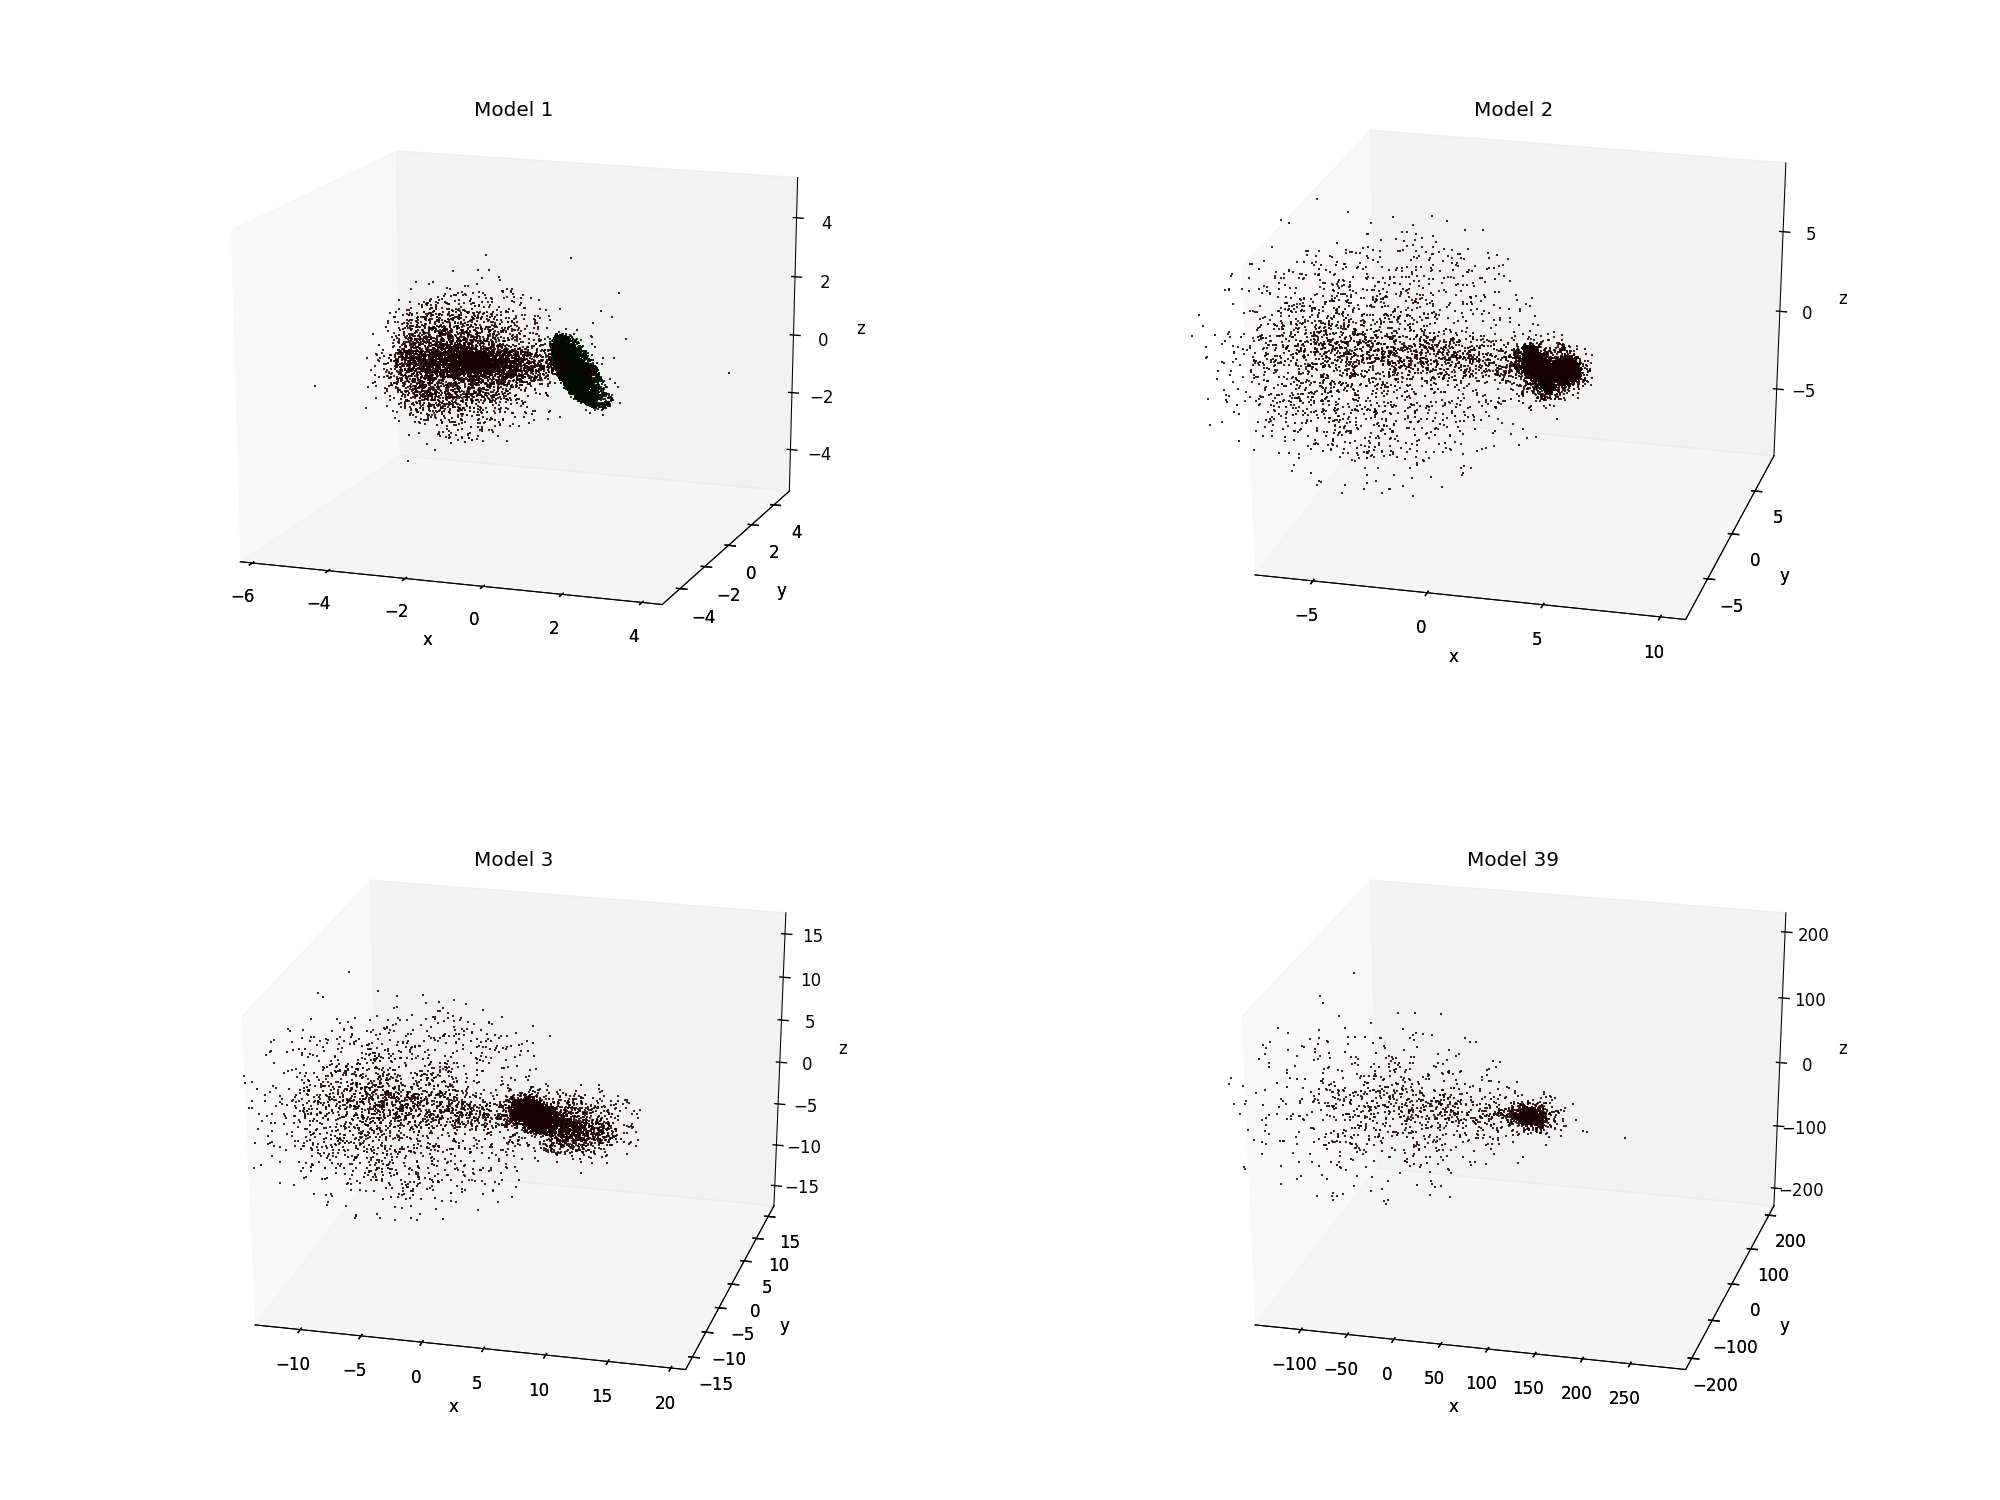
\includegraphics[scale=0.2]{240deg-m.png}
 \caption{\emph{ ángulo = 240 grados, los 2 objetos(solo parte luminosa) modelo 1,2,3,39 }}
\end{figure}

\begin{figure}[!ht]
 \centering
 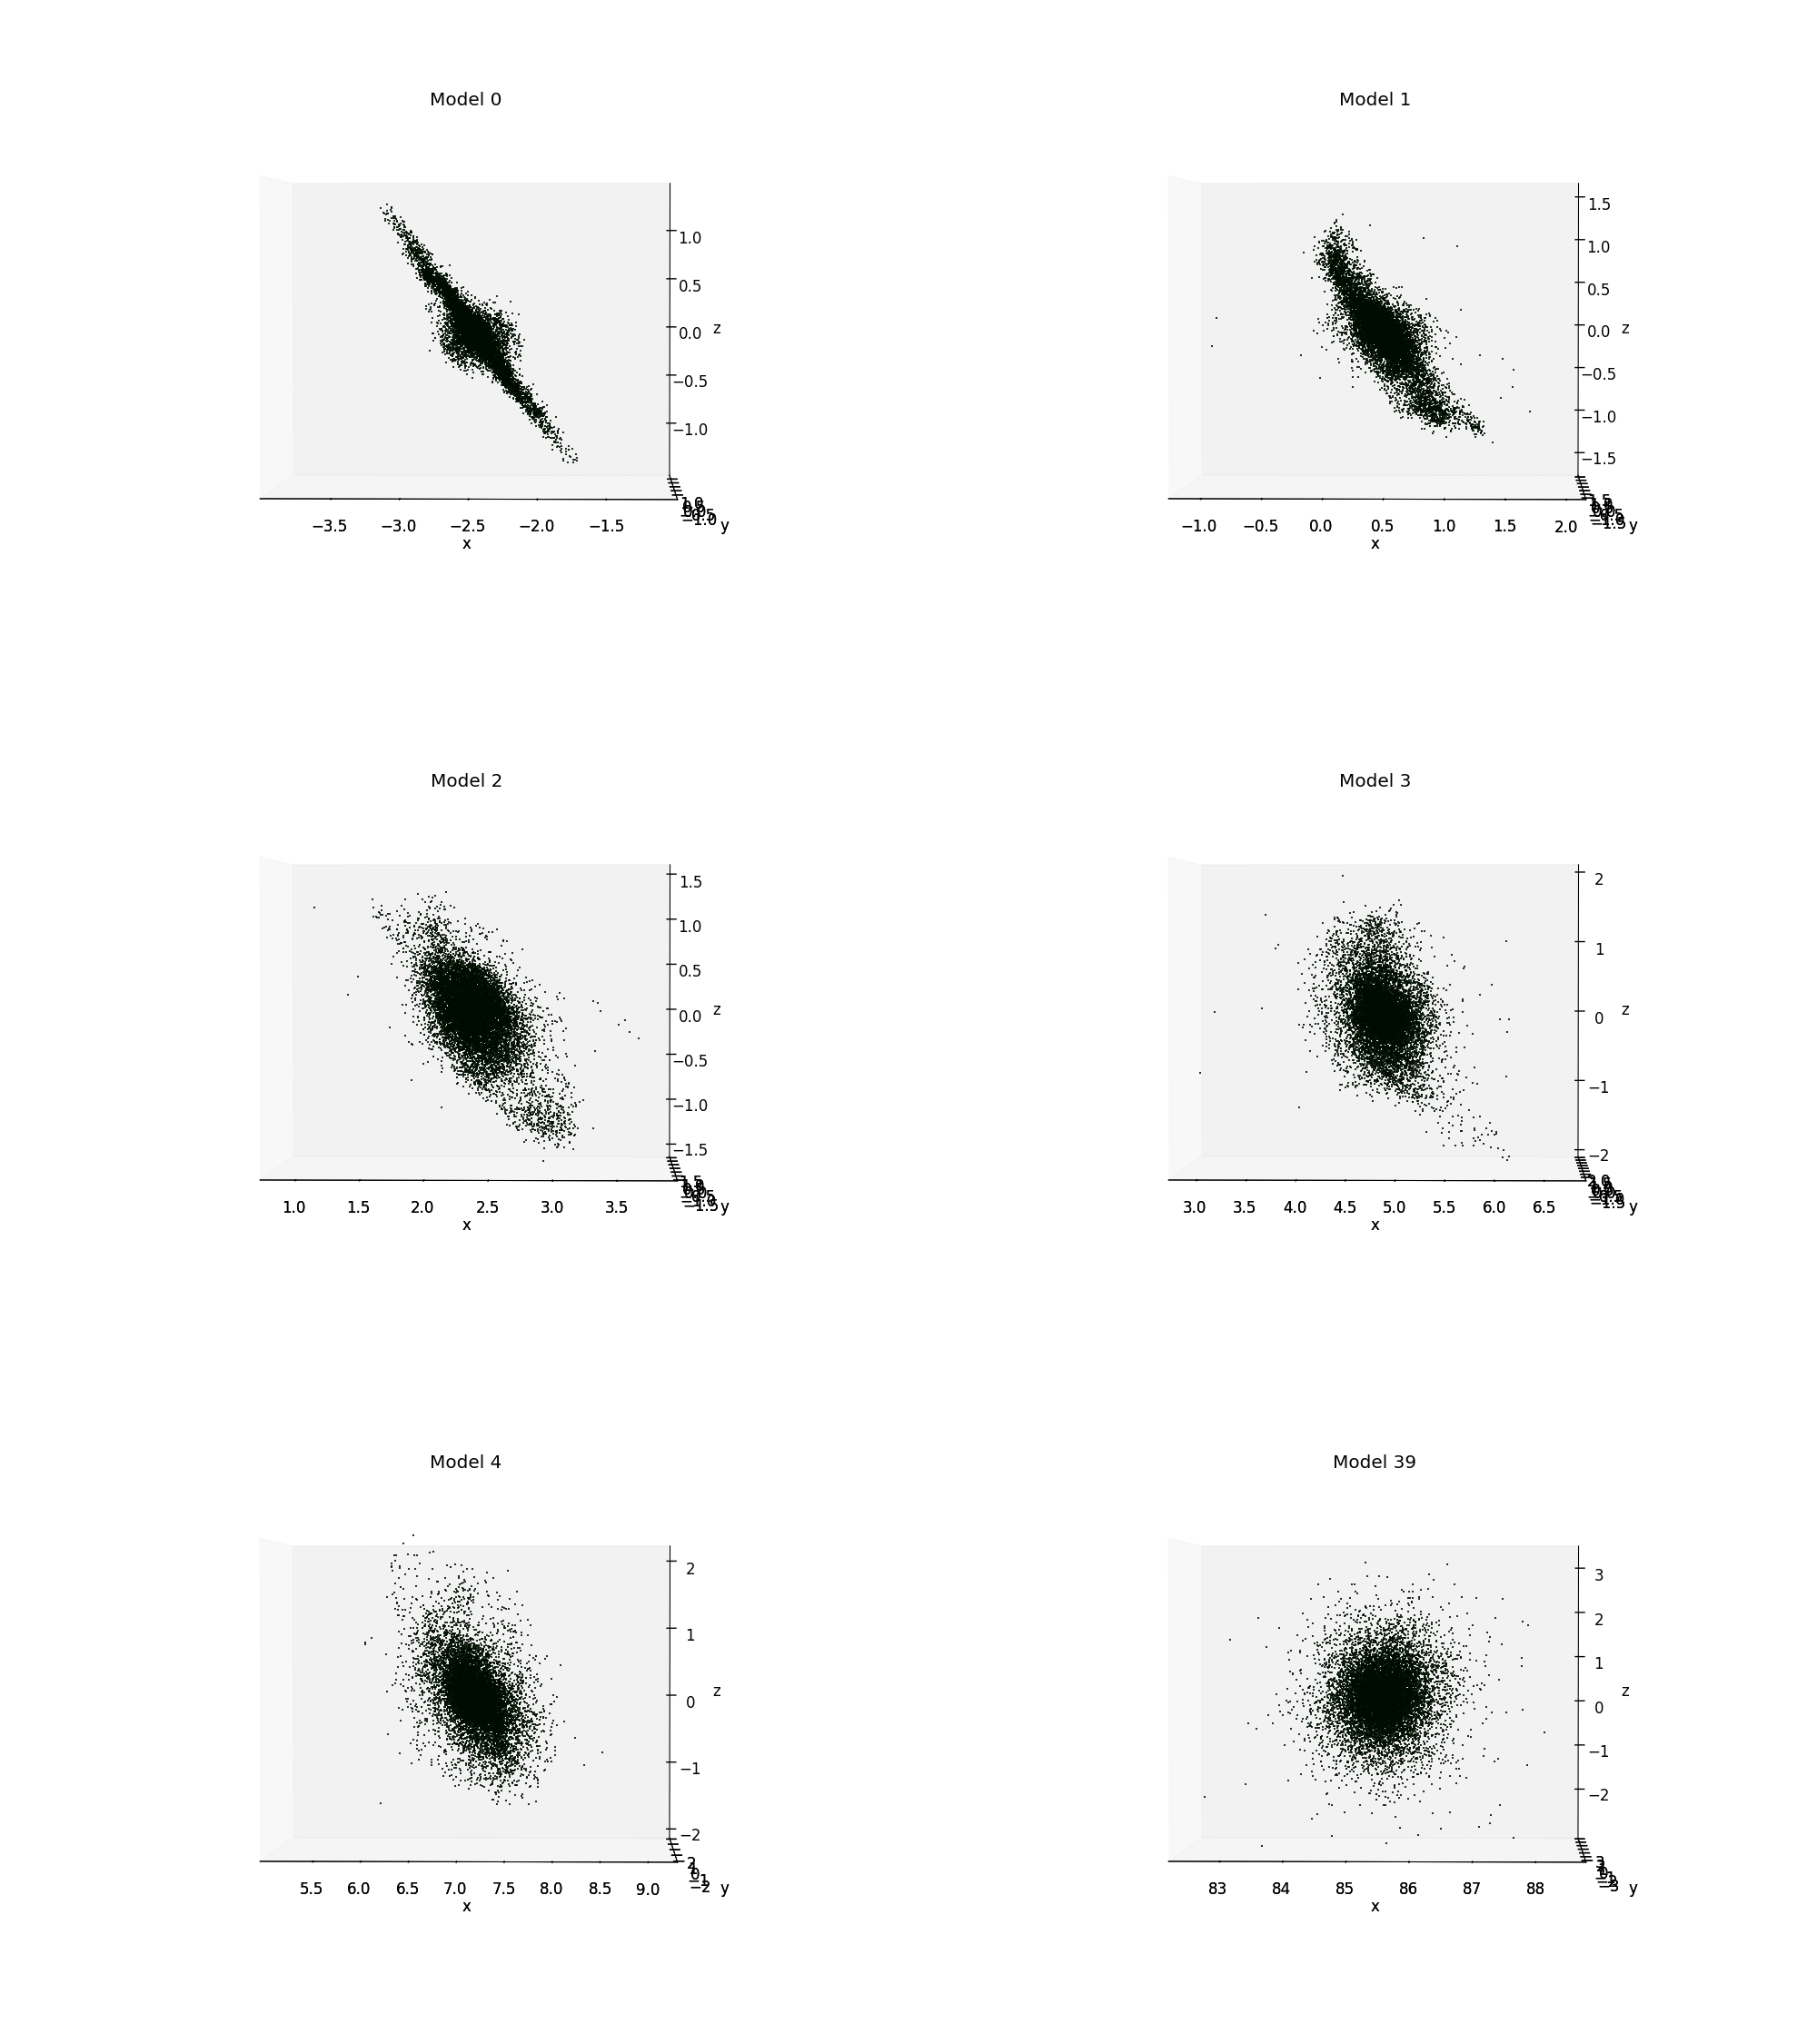
\includegraphics[scale=0.2]{240deg-m-c2y.png}
 \caption{\emph{ ángulo = 240 grados, el objeto con disco visto en la dirección oy(solo parte luminosa) modelo 0,1,2,3,4,39 }}
\end{figure}

\clearpage


\begin{figure}[!ht]
 \centering
 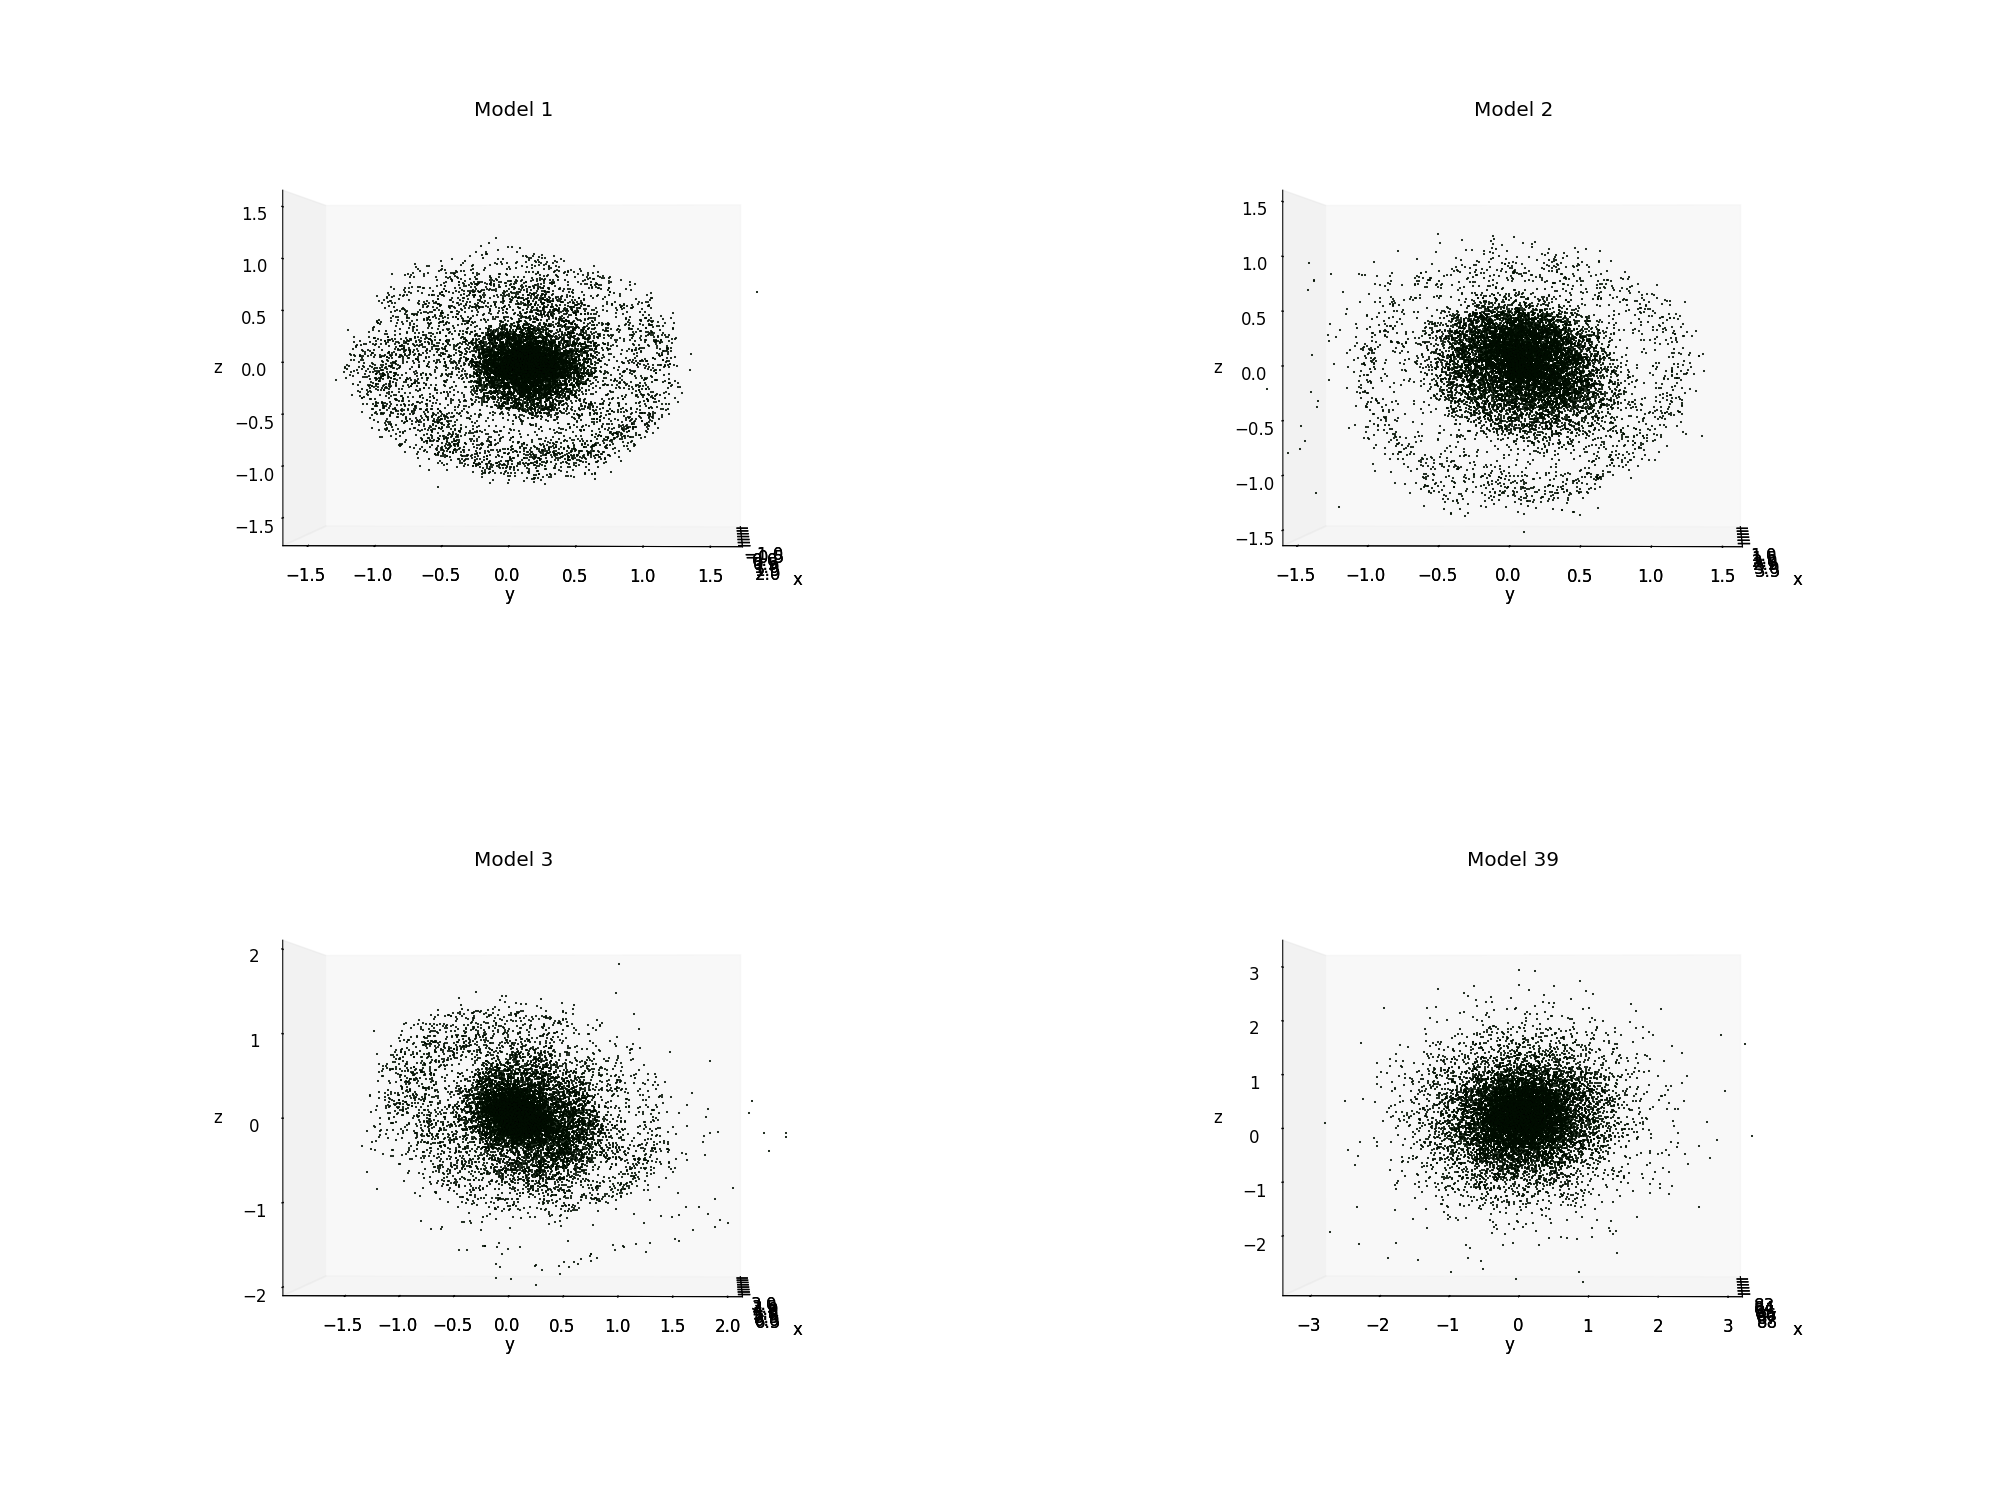
\includegraphics[scale=0.2]{240deg-m-c2.png}
 \caption{\emph{ ángulo = 240 grados, el objeto con disco visto en la dirección ox(solo parte luminosa) modelo 1,2,3,39 }}
\end{figure}

\begin{figure}[!ht]
 \centering
 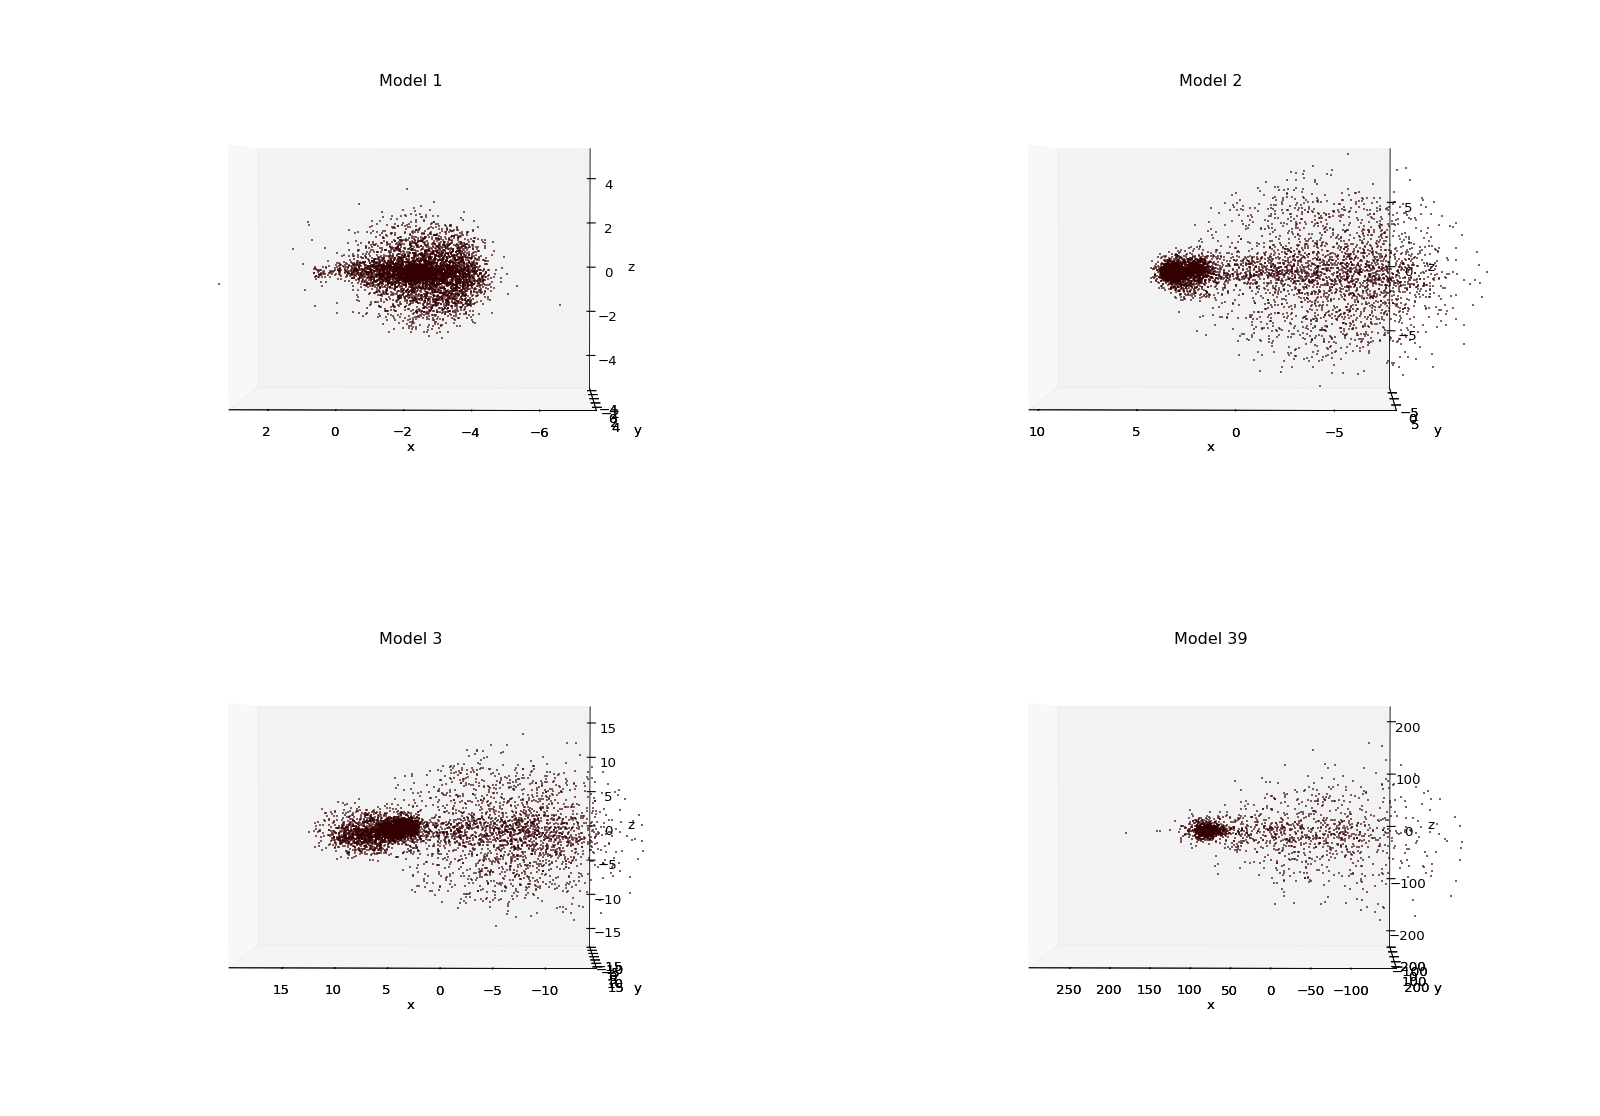
\includegraphics[scale=0.2]{sep5-240deg-eoy.png}
 \caption{\emph{ ángulo = 240 grados, el objeto esférico visto en la dirección oy(solo parte luminosa) modelo 1,2,3,39 }}
\end{figure}

\begin{figure}[!ht]
 \centering
 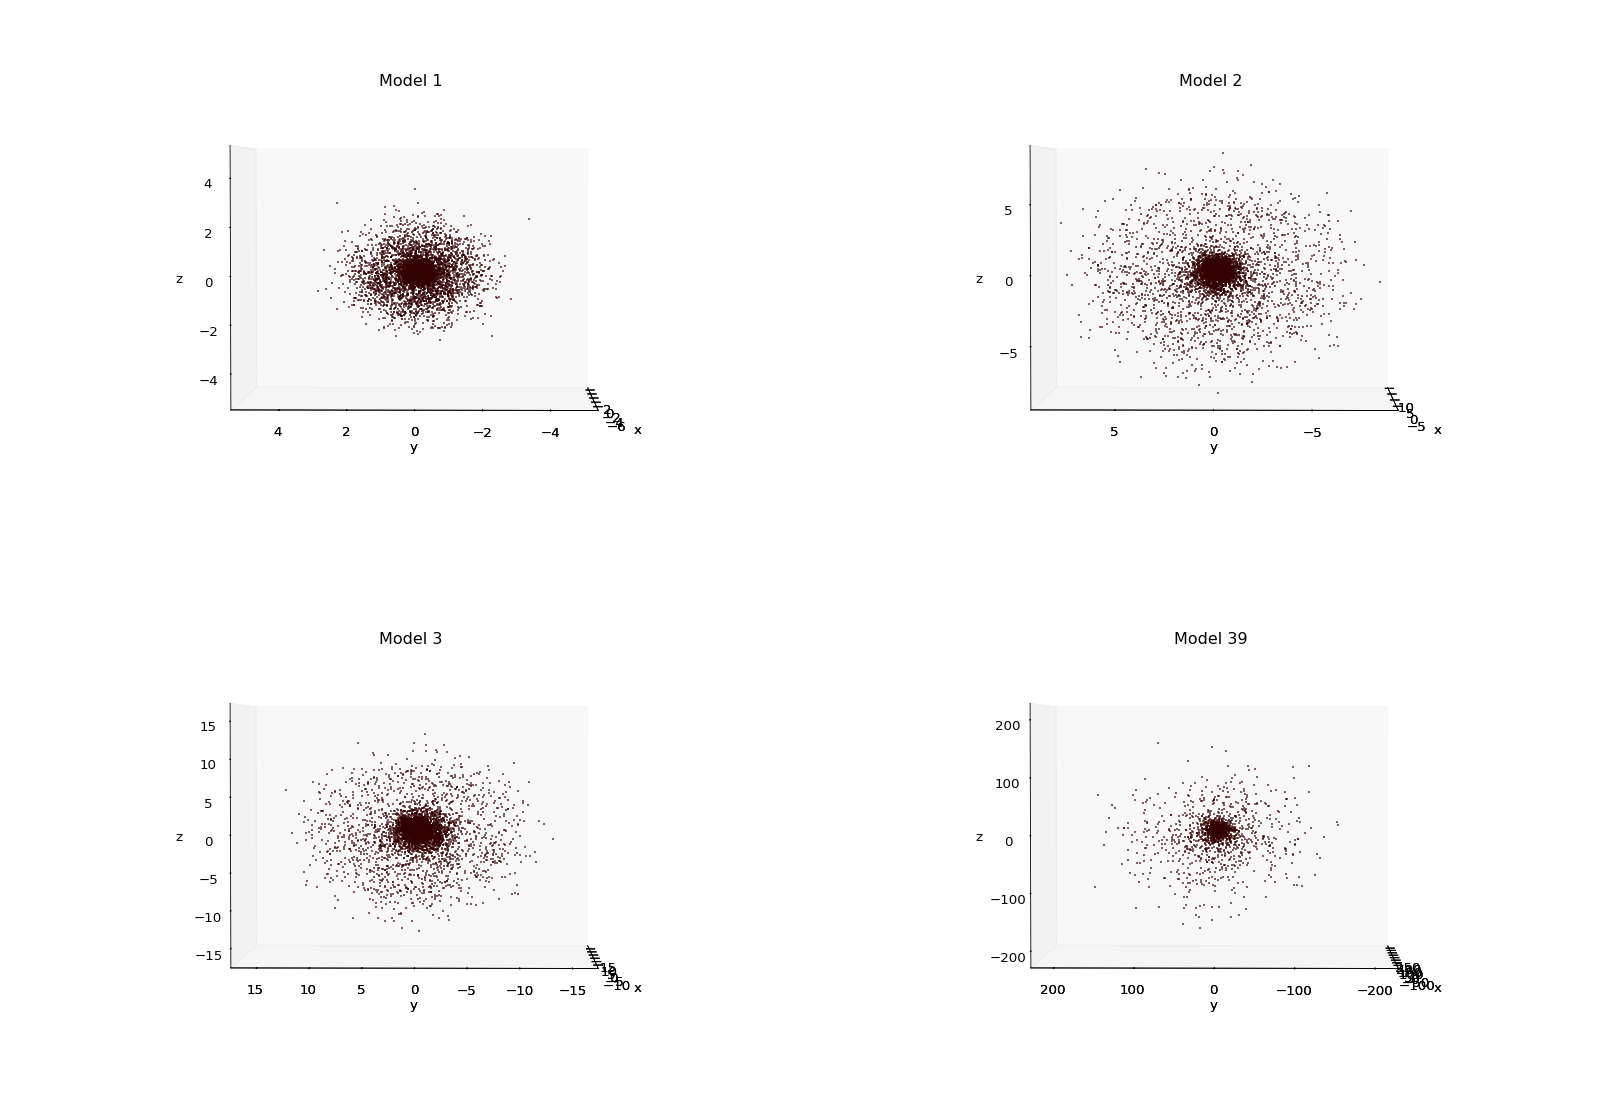
\includegraphics[scale=0.2]{sep5-240deg-eox.png}
 \caption{\emph{ ángulo = 240 grados, el objeto esférico visto en la dirección ox(solo parte luminosa) modelo 1,2,3,39 }}
\end{figure}



\begin{figure}[!ht]
 \centering
 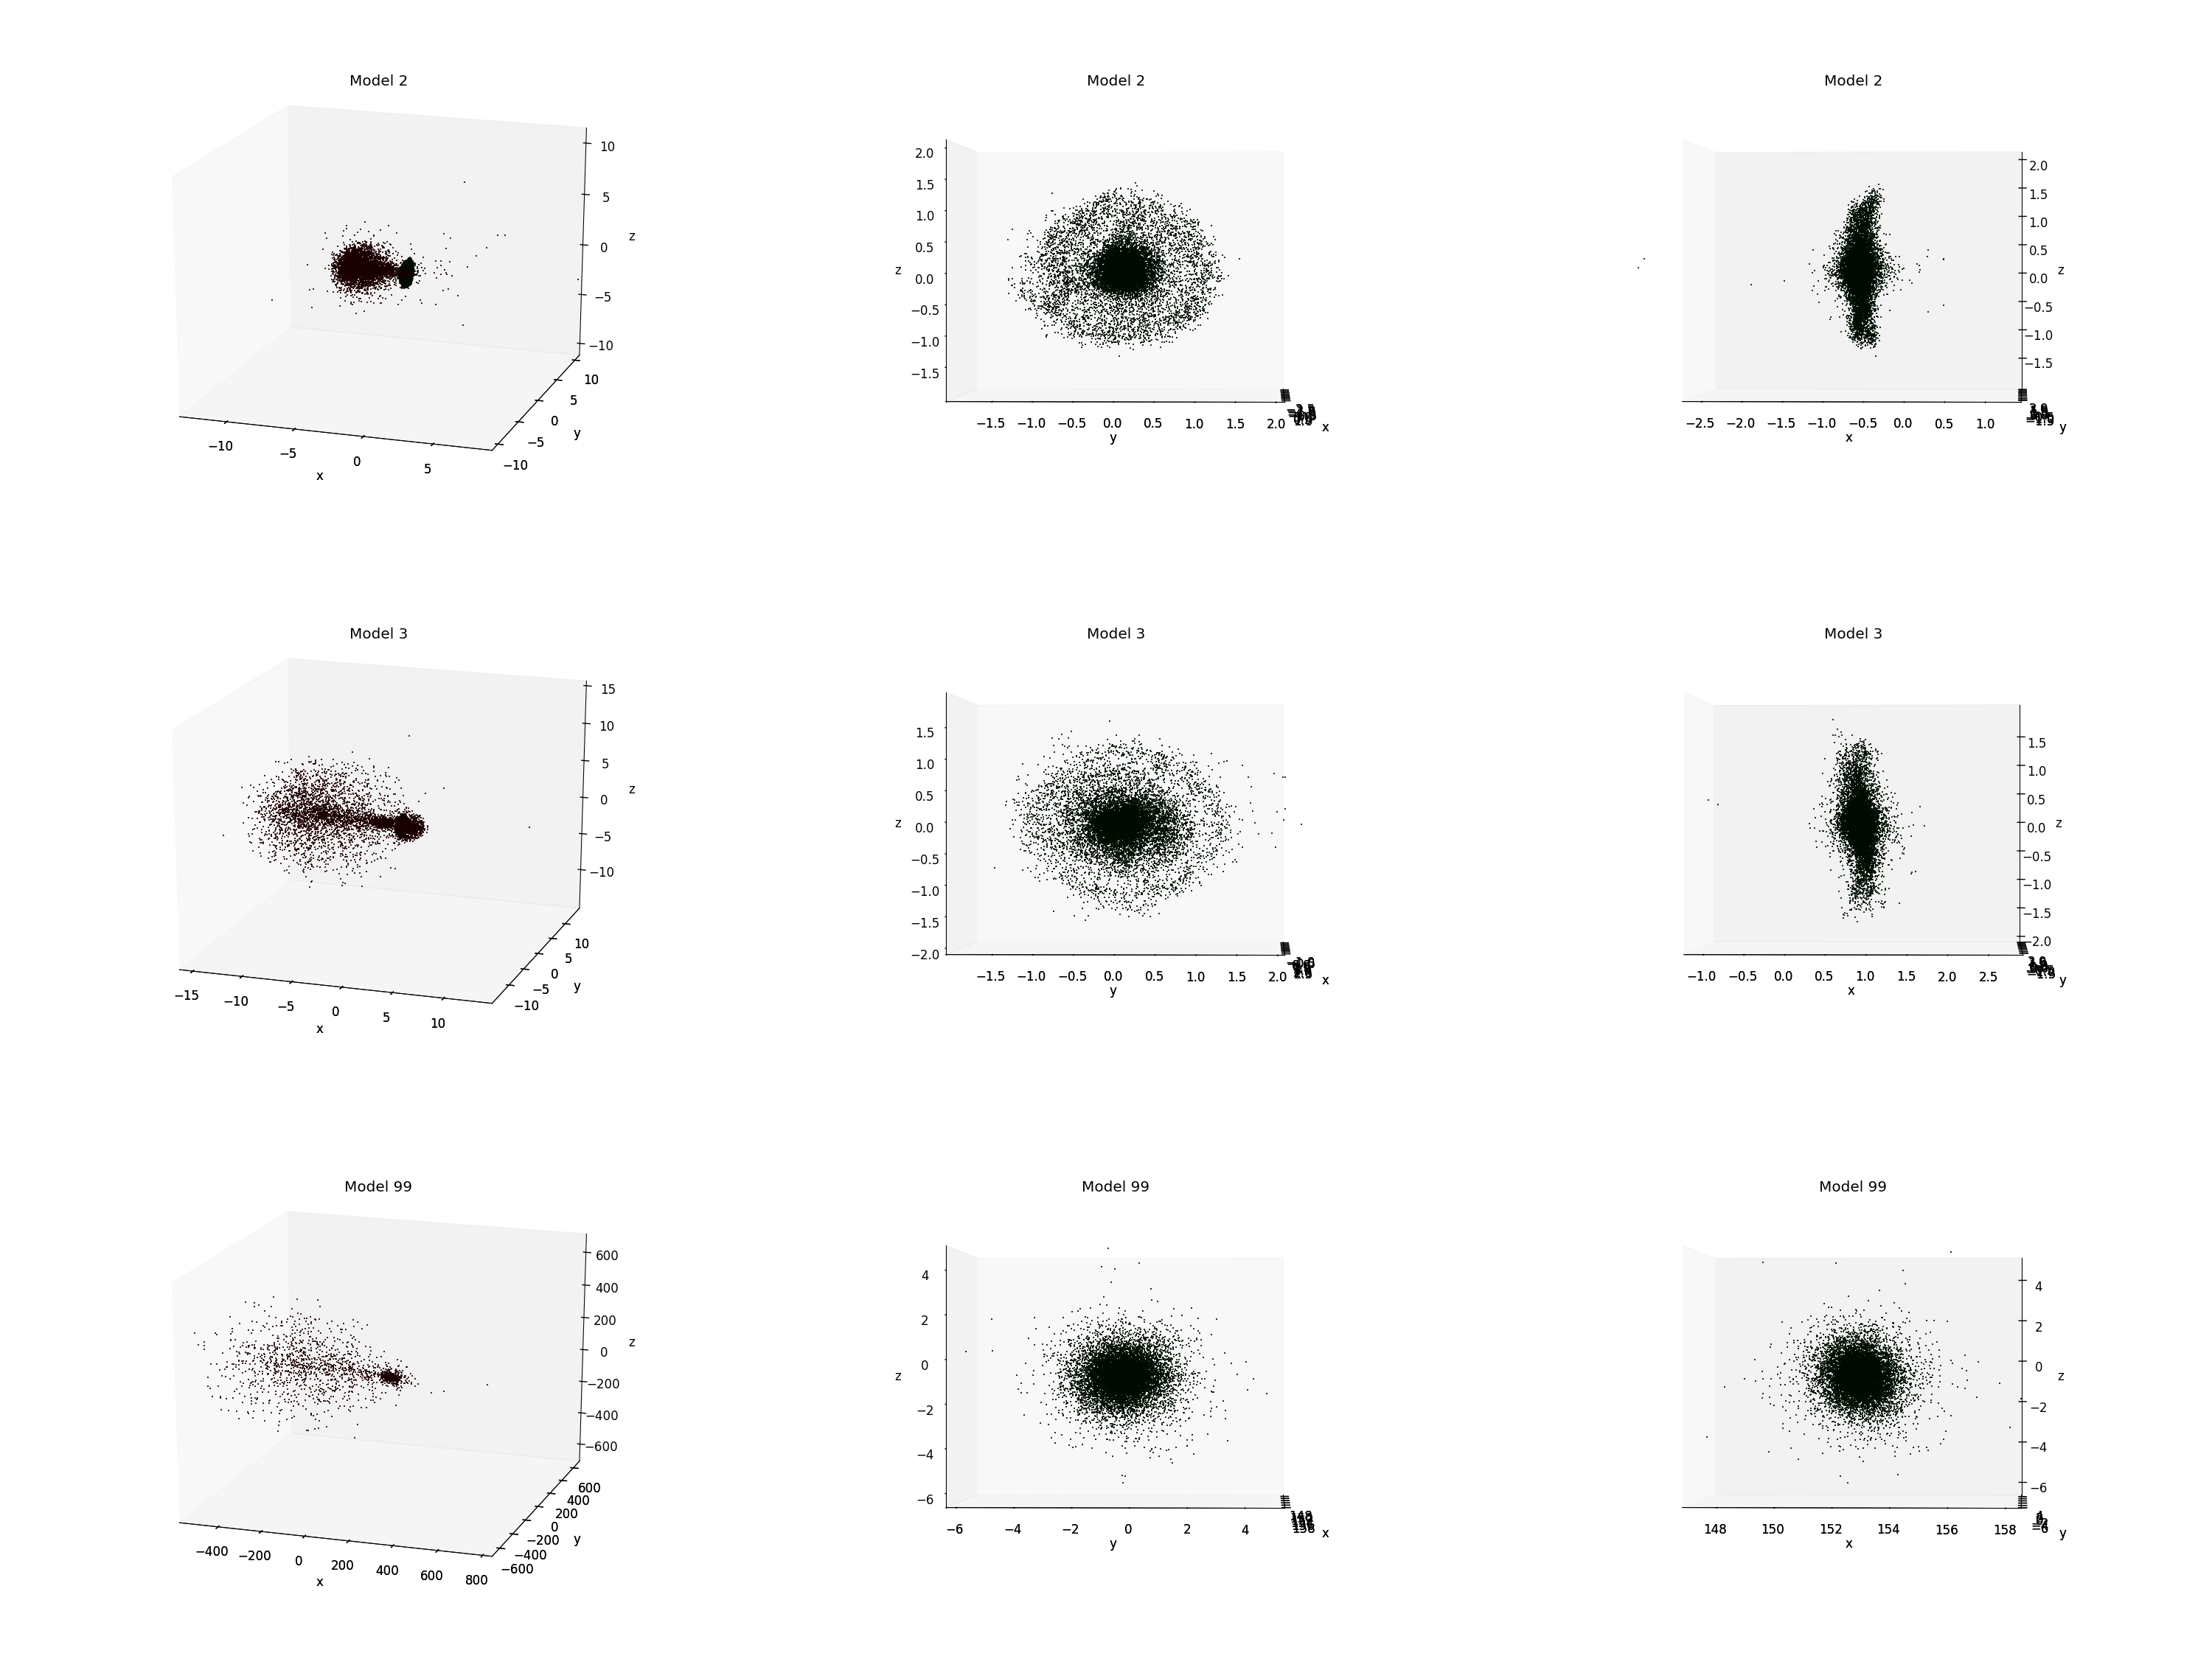
\includegraphics[scale=0.2]{sep10.png}
 \caption{\emph{ Separación = 10 , ángulo = 90 grados, solo la parte luminosa, primera columna los 2 objetos, la segunda el objeto con disco visto en la dirección ox, la tercera el objeto con disco visto en la dirección oy, modelos 2,3,99 }}
\end{figure}


\begin{figure}[!ht]
 \centering
 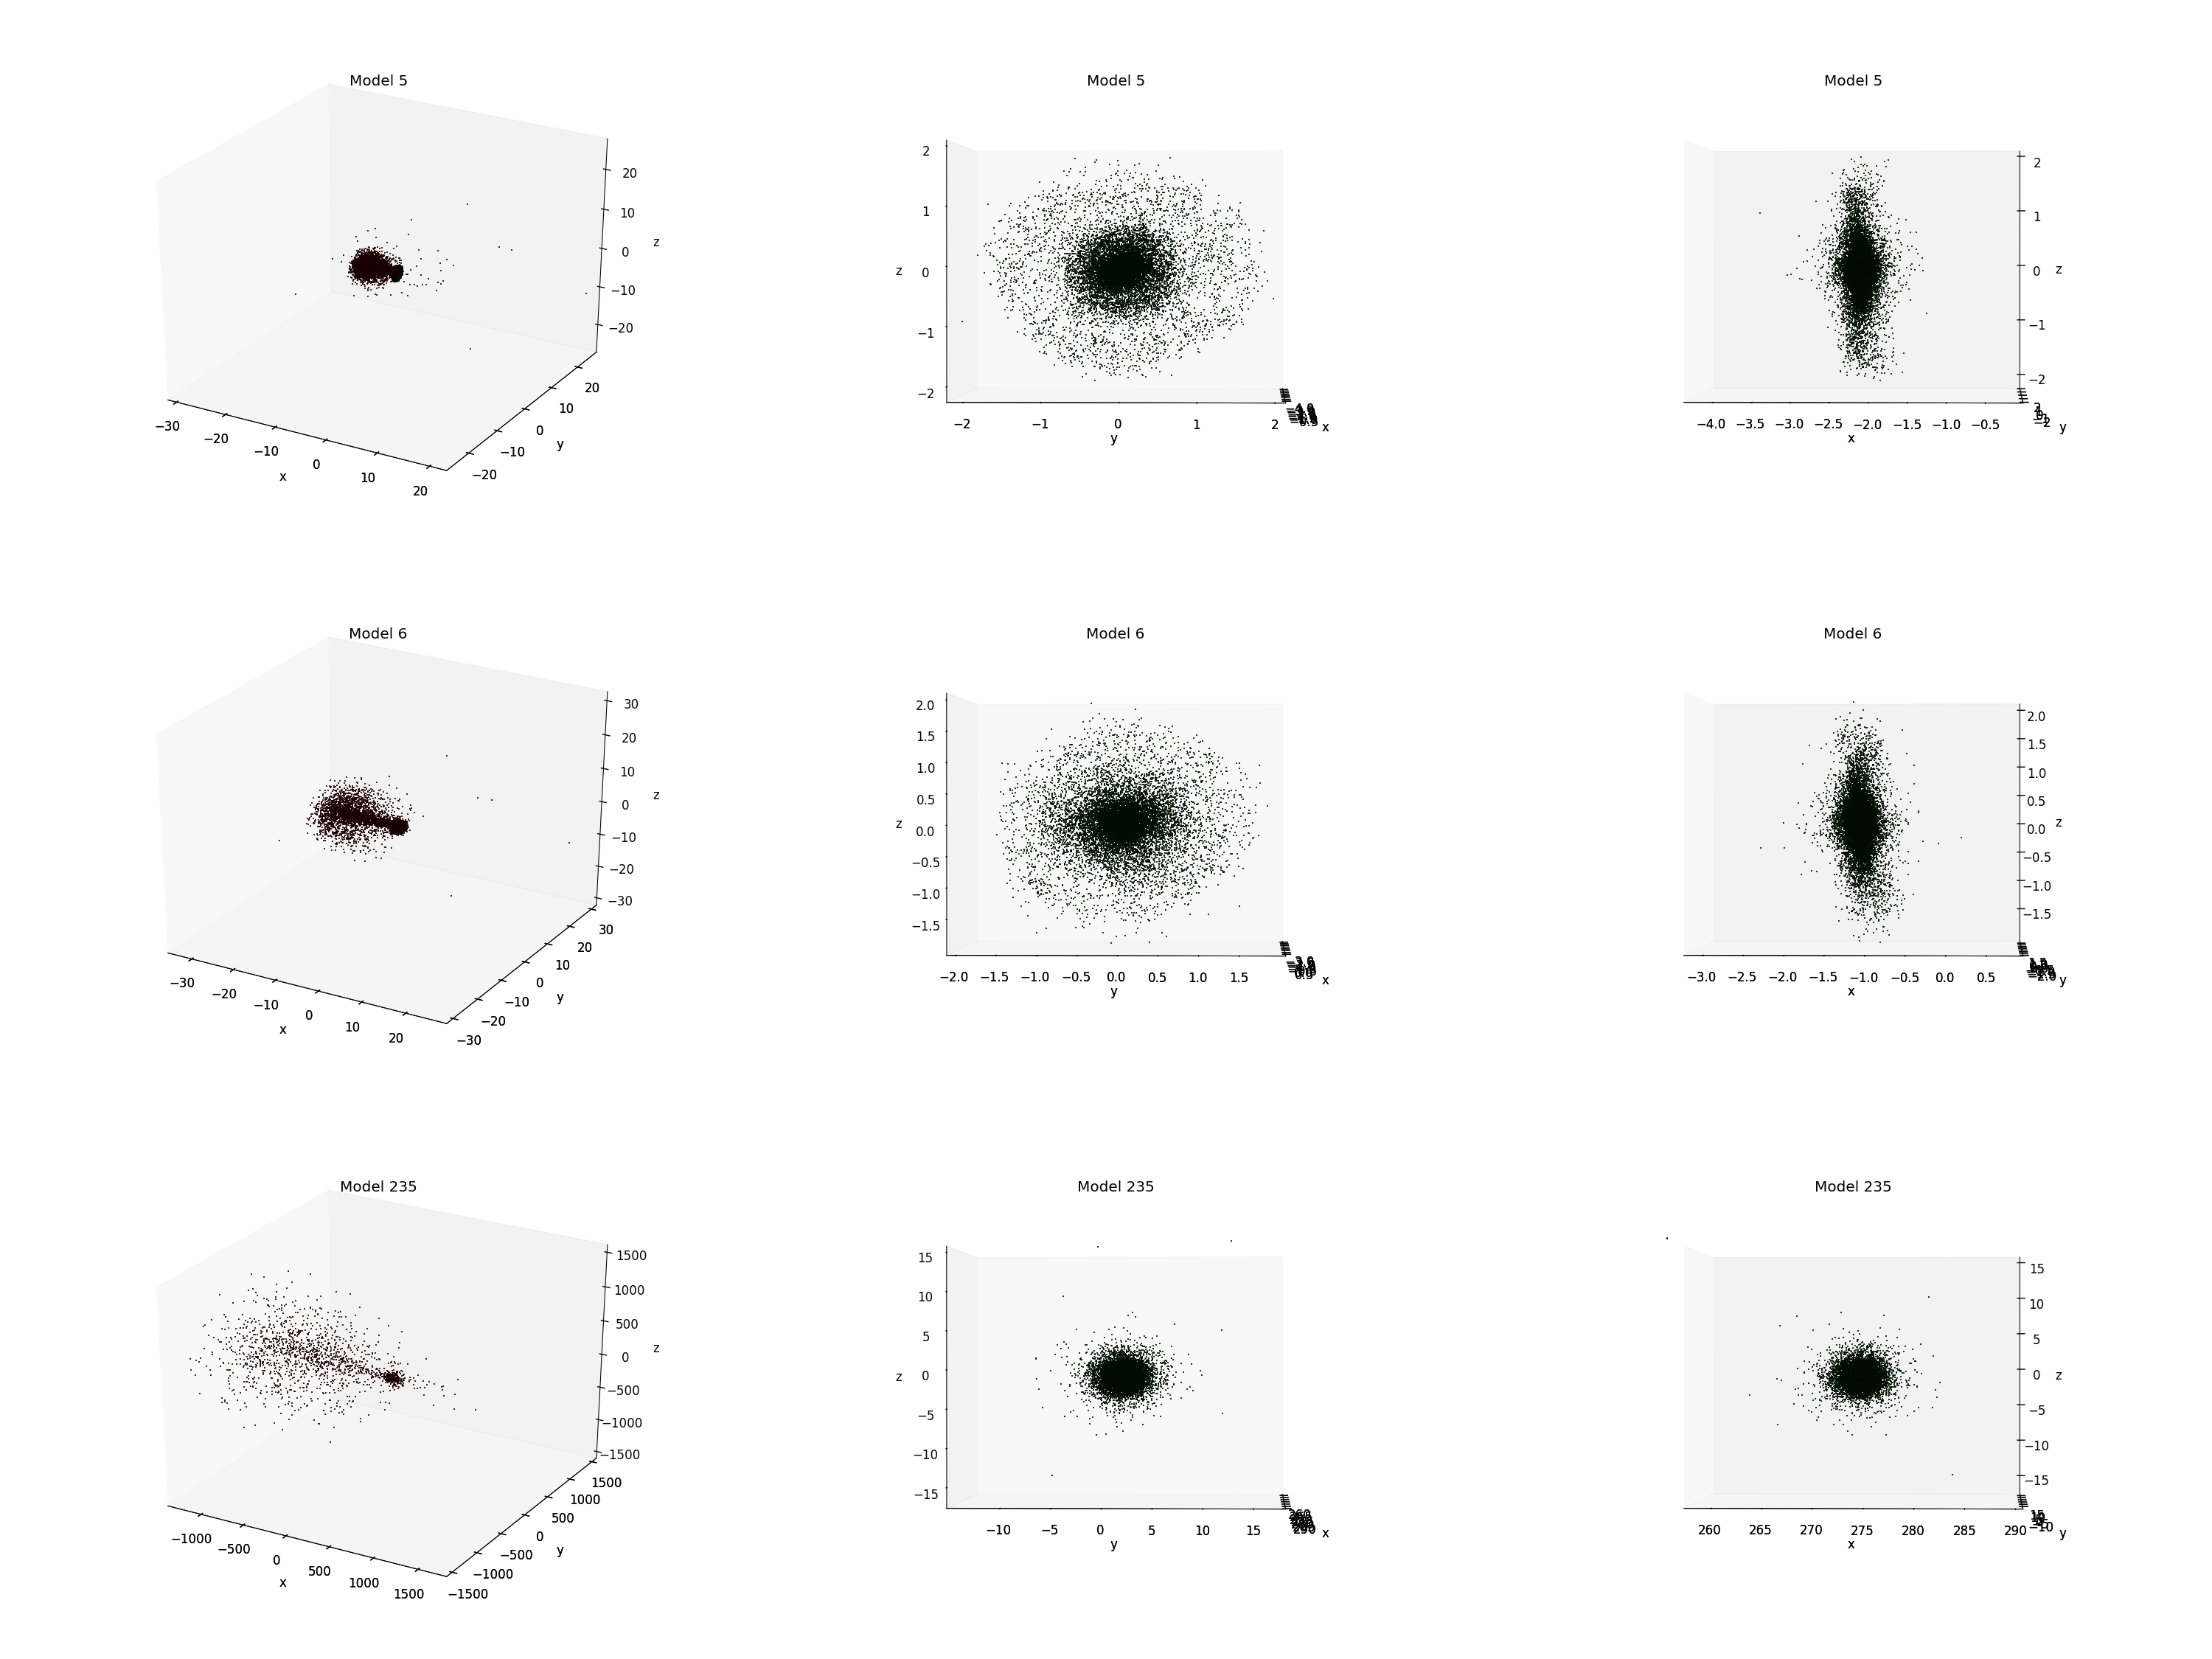
\includegraphics[scale=0.2]{sep20.png}
 \caption{\emph{ Separación = 20 , ángulo = 270 grados,solo la parte luminosa, primera columna los 2 objetos, la segunda el objeto con disco visto en la dirección ox, la tercera el objeto con disco visto en la dirección oy, modelos 5,6,235 }}
\end{figure}

\clearpage
\newpage

En el primer encuentro el objeto esférico va a atravesar el disco atrayendo partículas de este:
la forma curvada de los brazos espirales se estropea después del primer encuentro, 
haciendo que la parte luminosa del objeto con disco se parezca a una rueda de caro al largo de ox: explicación para la galaxia Cartwheel. 

Cuando el disco es perpendicular al plano de la órbita (ángulo = 90, 270) 
durante la evolución los objetos tienen simétria cási radial vistos al largo de la línea ox y simetría con respecto al axis oz vistos en el plano xoz y al axis oy vistos en el plano xoy.

Cuanto menor es la separación inicial el objeto esférico es más compacto y va a deformar mas el disco en la dirección ox y hasta una distancia menor desde el centro: el anillo hueco con los brazos de la rueda es mas extenso, pero mas difuso para una separación mayor

Para ángulos theta1 = 60 y 270 grados el objeto con disco no tiene más simetría con respecto al axis oz en el plano xoz
(hay una cola que se forma en la parte de abajo($z<0$) en la dirección ox) 
y porque la velocidad de rotación del disco va a tener una componente en la dirección ox que se va a sumar o restar a la 
velocidad del otro objeto mas pequeño dependiendo del sentido de rotación el disco se va a alabear en la dirección 
positiva de ox para $y > 0$ cuando el ángulo = 240 grados  y para $y<0$ cuando el ángulo = 60 de grados,
pero vistos en el plano yoz el disco para angulo = 60deg es casi 
antisimétrico al disco para ángulo = 240deg con respecto al axis oz ($y_{60deg} = -y_{240deg} $)

En los encuentros posteriores las partículas que no se han escapado definitivamente  en el primer encuentro(solo se escapan partículas del objeto esférico - como se vera más adelante) van a tener menor velocidad y el anillo cartwheel va a desaparecer. 


\subsection*{Análisis para el caso separación = 5, ángulo = 90}


\paragraph{Equilibrio hidrostático}
El sistema no alcanza el equilibrio. Miramos el gráfico del radio para varios valores de la fracción de masa y comprobamos si se cumple T. virial

\begin{figure}[!ht]
 \centering
 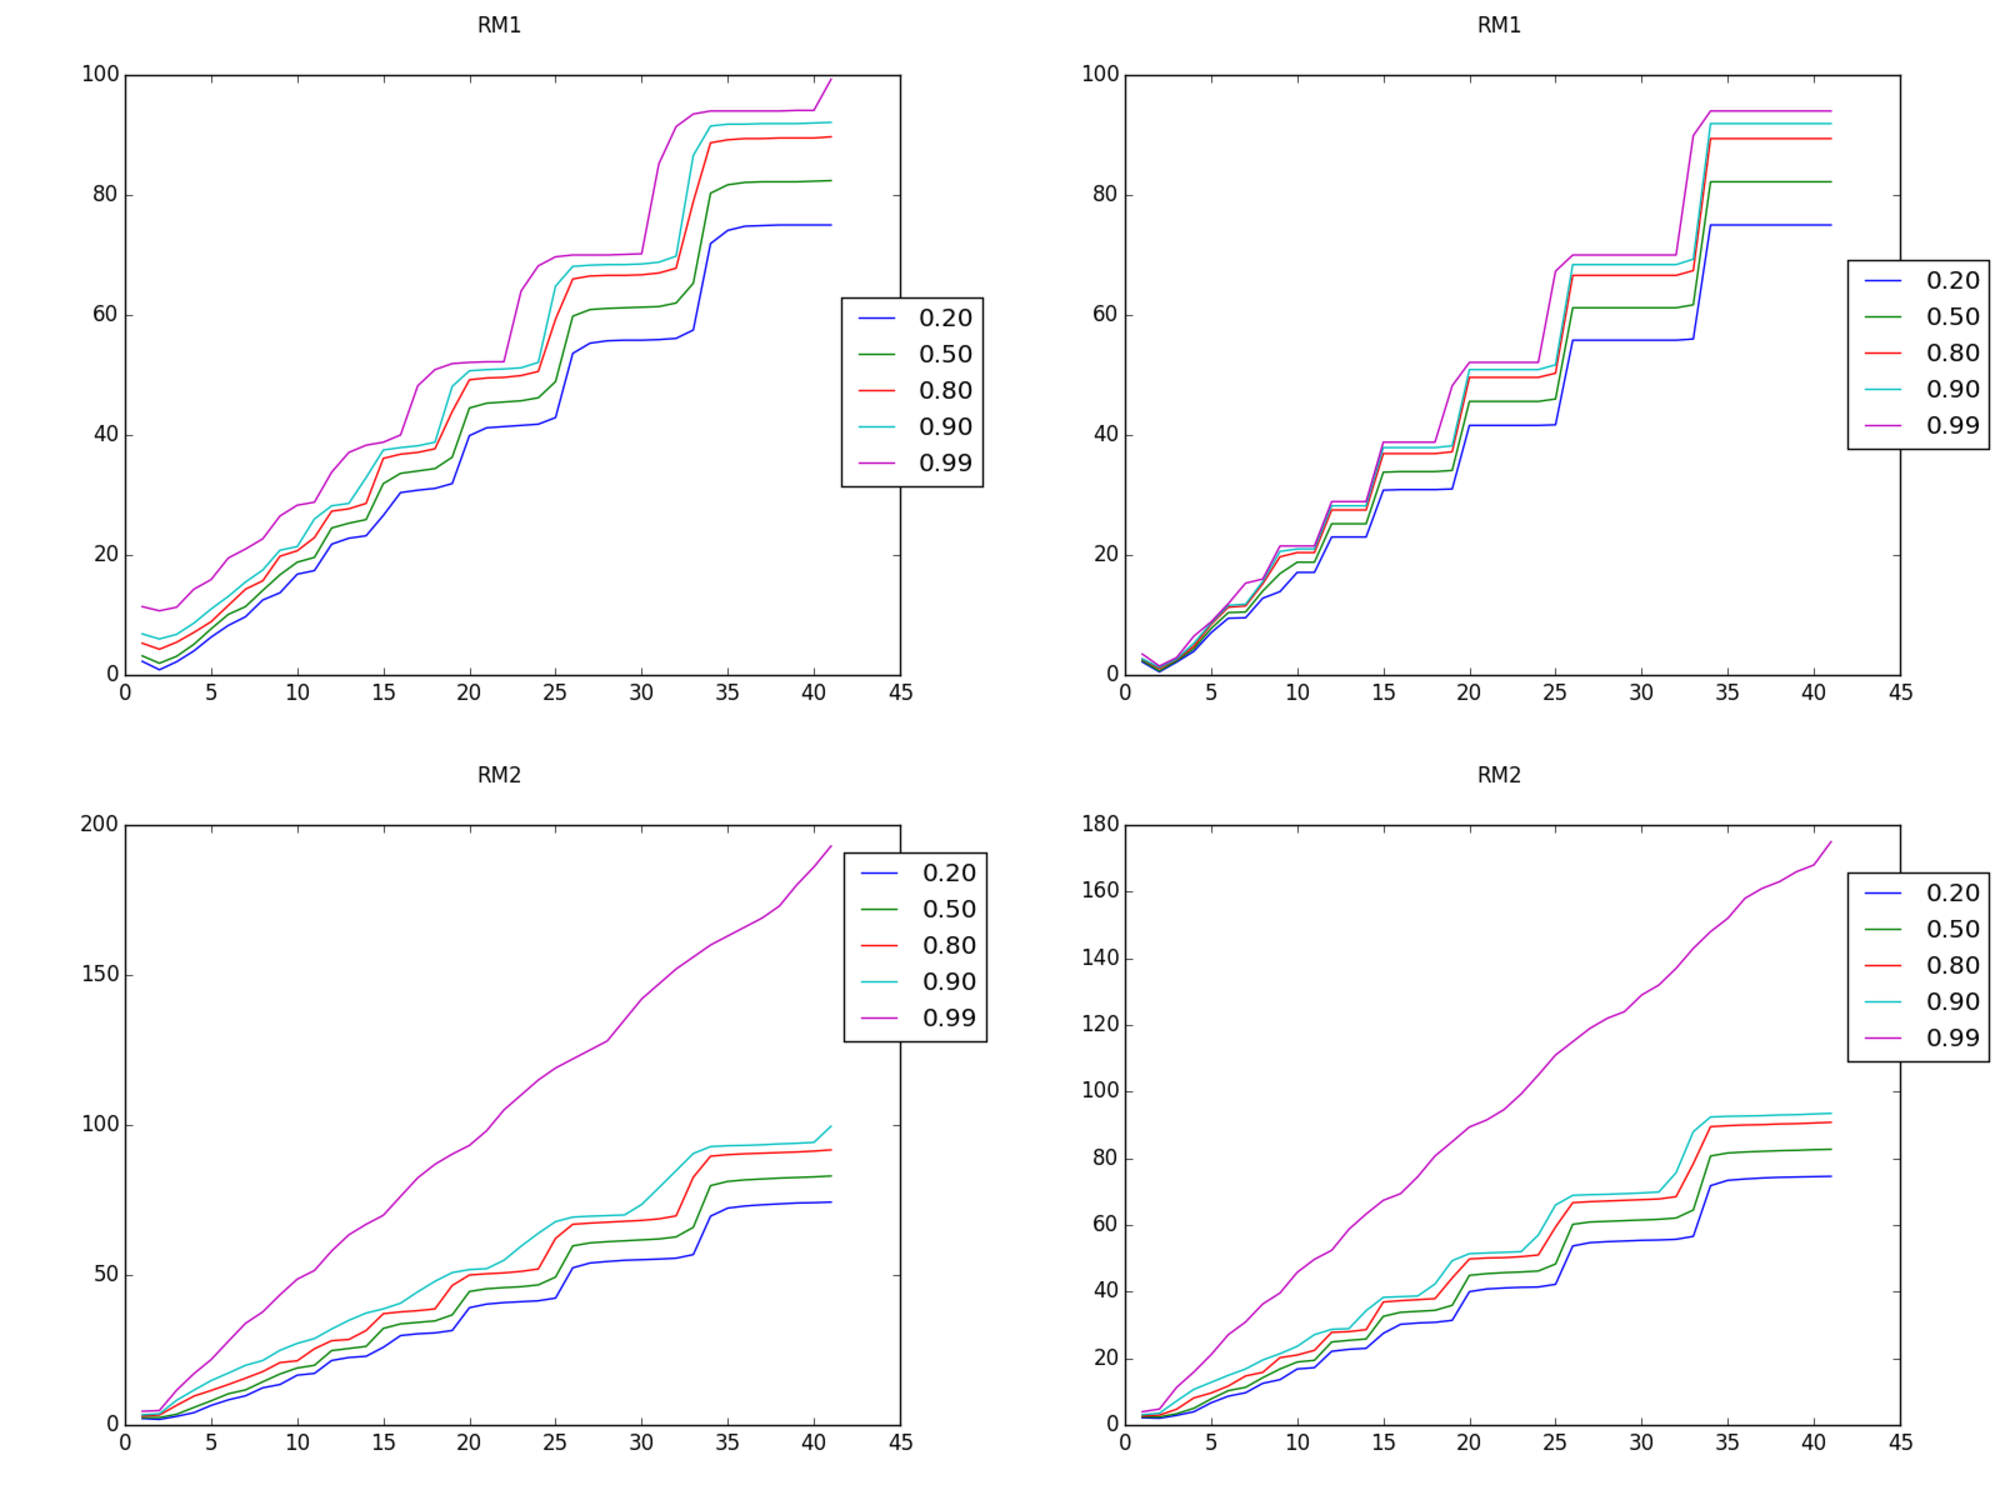
\includegraphics[scale=0.2]{rmsep5.png}
 \caption{\emph{Rm obtenido en nora: primera fila el objeto con disco, la segunda el modelo esférico, la primera columna el objeto entero, la segunda solo la parte luminosa }}
\end{figure}

En realidad el objeto con disco no se expande tanto: algunas partículas se escapan, pero el disco se hace cada vez mas grueso hasta que se convierta  en  una esfera con el radio 1-2 veces mayor  al radio inicial del disco. 
Creo que nora tiene en cuenta la posición inicial de las partículas en el output de Rm

Mirando Ebind en nora vemos que del objeto con disco se escapan mucho menos partículas que en el objeto esférico (porque es mas masivo y tiene mas energia  de ligadura). 

Las partículas del objeto con disco que se escapan van orbitando alrededor de centro de masas cada vez a radio mayor igual que algunas partículas del modelo esférico (por eso la forma de escalera de los gráficos de Rm en función de tiempo).
 
Pero en el modelo esférico hay algunas partículas que se encuentran en el momento incial en la parte exterior (entre radio masa 90\% - 99\% ) que se van alejando constantemente del centro de masas después del primer encuentro: por eso la línea recta para el radio de la fracción de masa 99\% en el modelo esférico y la cola  que se ve en Ebind para el modelo esférico.


\begin{figure}[!ht]
 \centering
 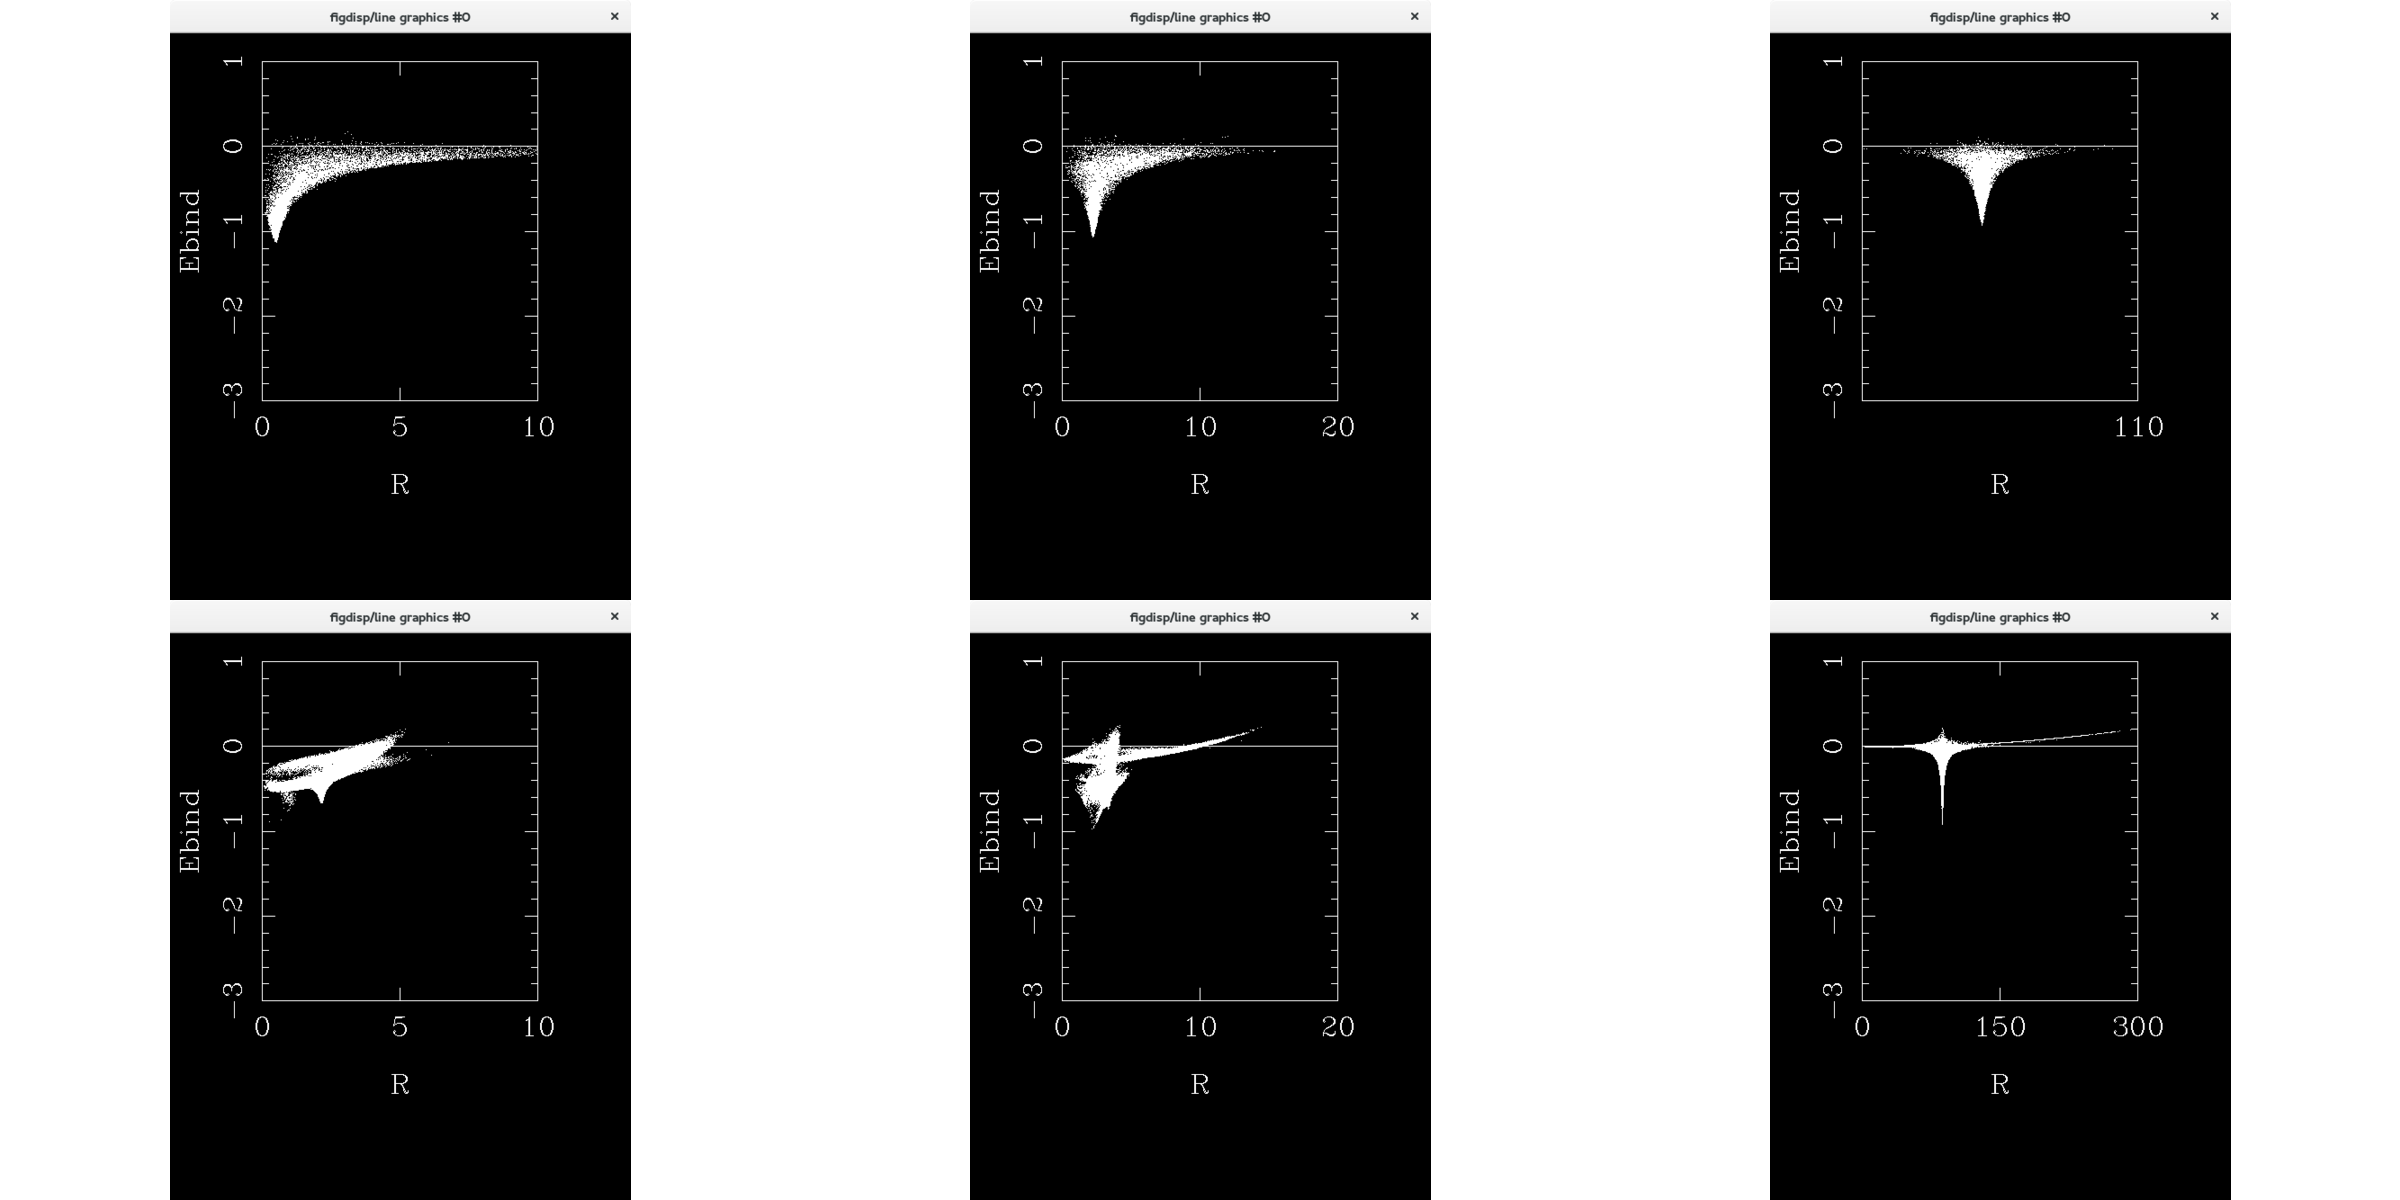
\includegraphics[scale=0.2]{ebindsep5.png}
 \caption{\emph{ Ebind en nora. La primera fila: el modelo con disco, la segunda el modelo esférico, las particulas con energía positiva se van a escapar. Las columnas representan modelo 1,2,40.
}}
\end{figure}

También se puede observar en las imágenes de la evolución la cola formada por las partículas del modelo esférico que se está alejando en la dirección -ox


\begin{figure}[!ht]
 \centering
 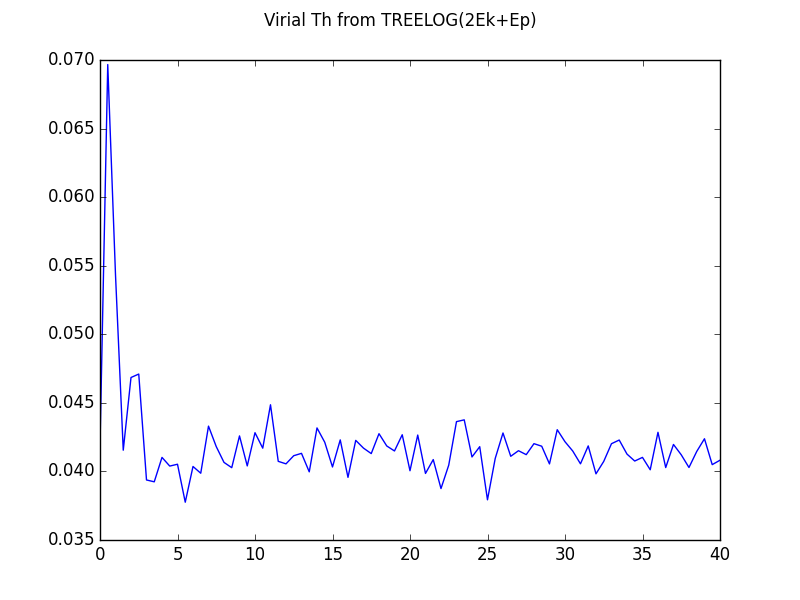
\includegraphics[scale=0.4]{vt.png}
 \caption{\emph{T. virial no se cumple (2Ek+Ep frente al tiempo)}}
\end{figure}

\clearpage

\paragraph{Objeto final(fusión)}

Como se ve en el zoom del modelo final las 2 galáxias fusionan en un objeto cási esférico + las partículas que se van escapando orbitando a radios cada vez mayores (son partículas principalmente del modelo esférico)
\begin{figure}[!ht]
 \centering
 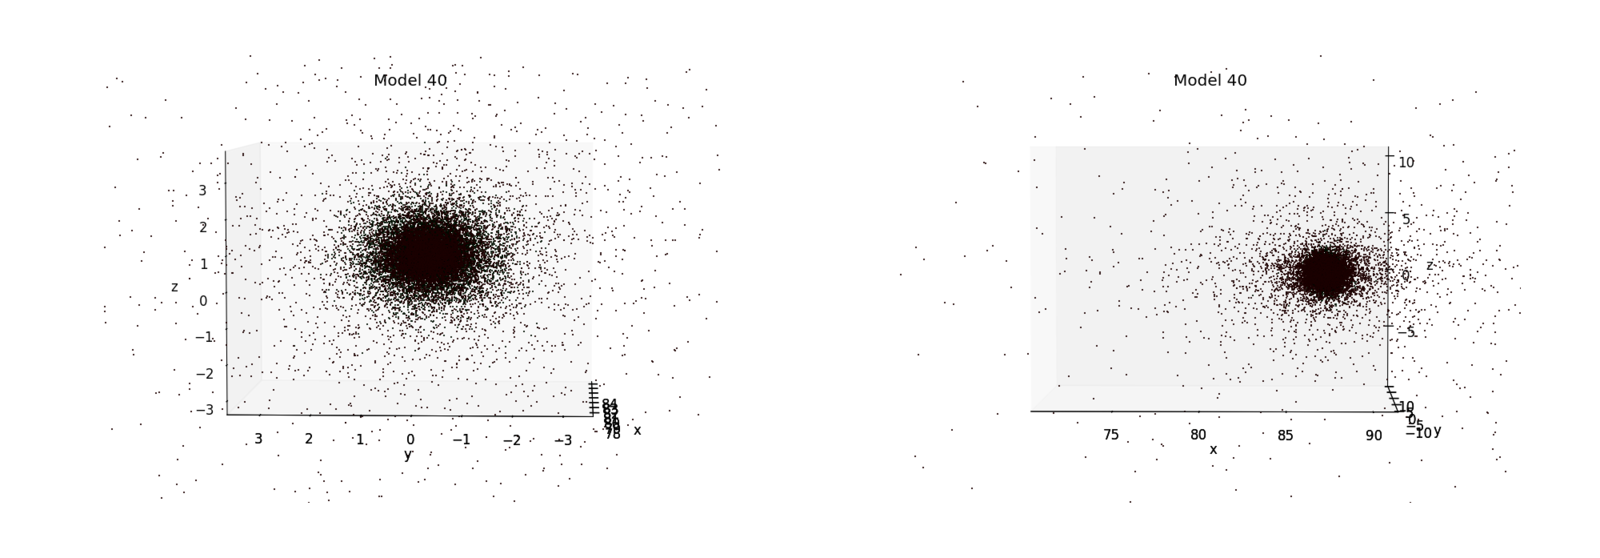
\includegraphics[scale=0.2]{finzoomsep590deg.png}
 \caption{\emph{zoom en el objeto final}}
\end{figure}

Miramos las distancias entre los centros de los 2 objetos:

\begin{figure}[!ht]
 \centering
 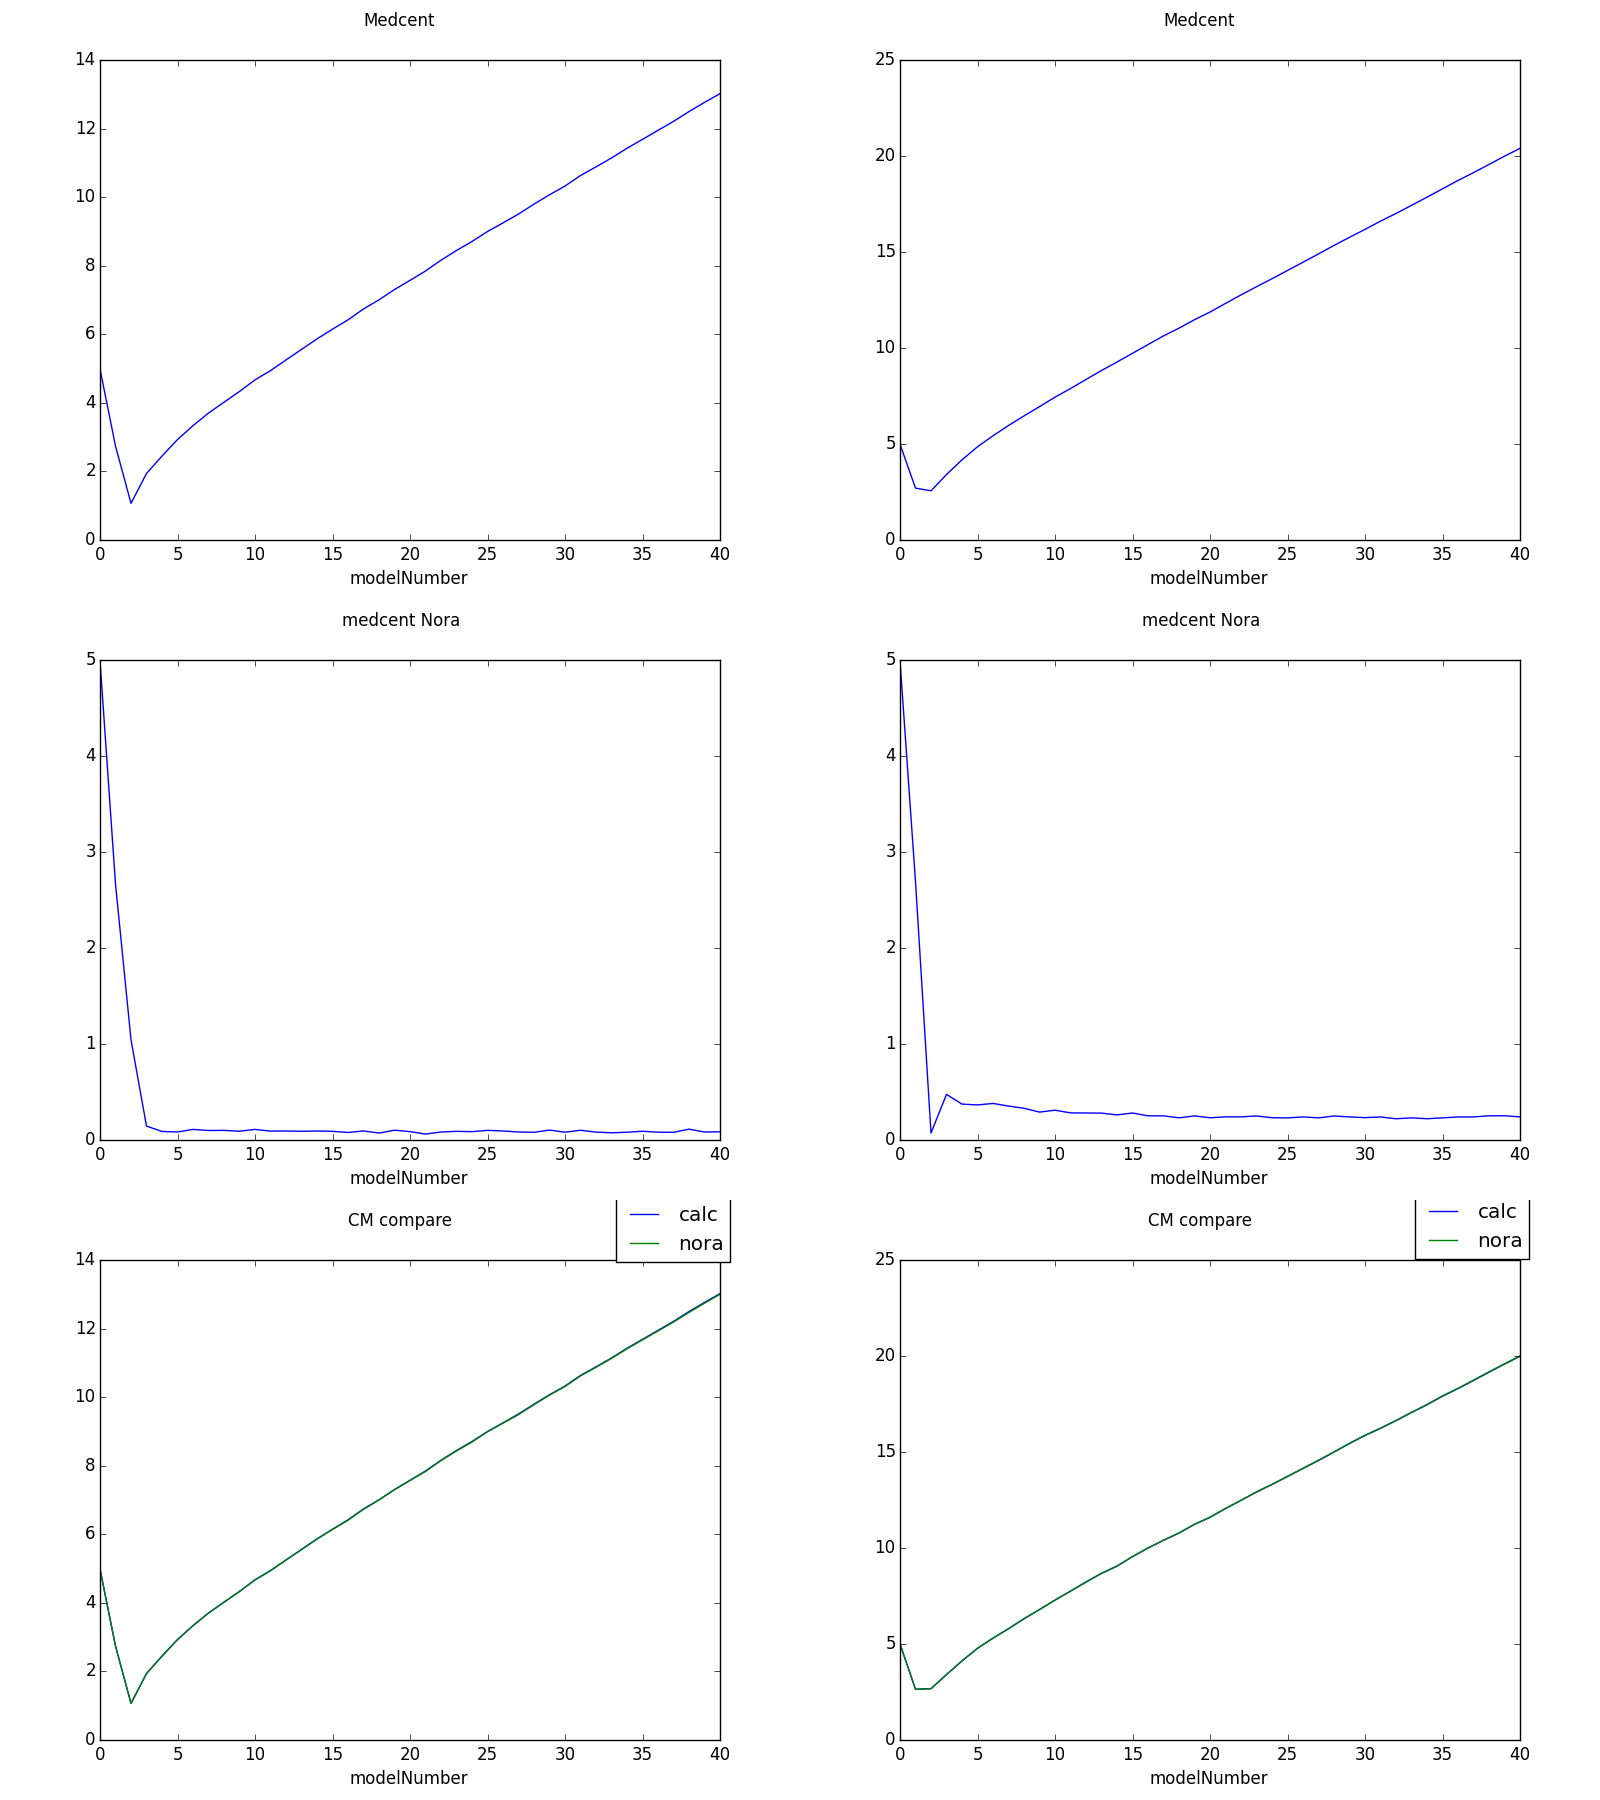
\includegraphics[scale=0.2]{sep5Centerdist.png}
 \caption{\emph{ distancia entre los centros: en la primera fila medcent en python, en la  segunda  medcent en nora y en la tercera cmcent(comparación entre los valores calculados en python y con nora); en la primera columna solo la parte luminosa, en la segunda incluyendo halo }}
\end{figure}

En python para cada objeto de los 2 he calculado $medcent = \frac{1}{N}\sum_i{r_i}$ donde N es el número total de partículas del objeto y $r_i$ las posiciones de las partículas del objeto, 
y $cmcent = \frac{1}{M}\sum_i{r_i m_i}$ donde M es la masa total del objeto, $r_i$ y $m_i$ son las posiciones y masas de las partículas del objeto.
Teniendo los 2 centros: c1 y c2 (calculados con medcent o cmcent) la distancia entre los 2 es $\sqrt{\sum_i{(c1_{x_i} - c2_{x_i})^2}}$
Los valores calculados con medcent en python  son diferentes a los obtenidos con medcent en nora(como se calculó allí?, los 2 objetos que contienen la mayor parte de las partículas se quedan a una distancia constante muy pequeña)
medcent en python y cmcent muestra la distancia creciendo constantemente, pero es por las partículas que se escapan



\clearpage
\paragraph{Es el objeto final una galáxia elíptica?}
Comprobamos si ahora la galáxia con disco se parece más a una \textbf{galáxia elíptica} mirando la relación del brillo superficial con $r^4$ y 
la dispersión de velocidad frente a la velocidad en nora(las galáxias elípticas tienen más dipersion de 
velocidad porque el movimiento es mas aleatorio a la diferencia del disco donde la velocidad es de rotación )

\begin{figure}[!ht]
 \centering
 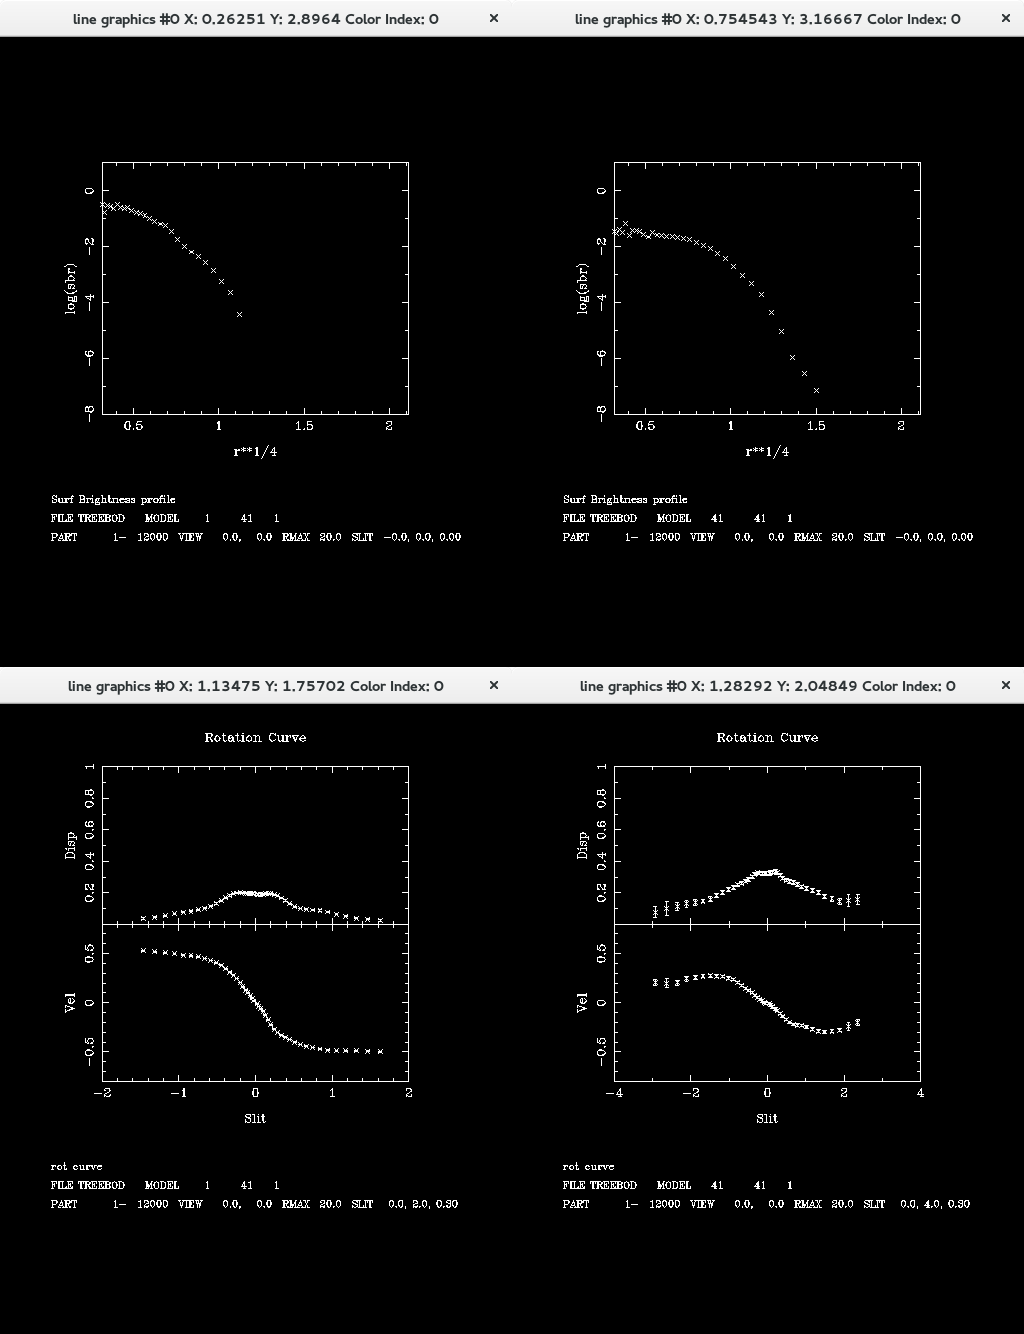
\includegraphics[scale=0.3]{noraellip.png}
 \caption{\emph{primera fila: sbr 2 2, segunda fila: rotc 0 radio 0.3, primera columna en el momento inicial, la segunda en el momento final, solo la parte luminosa  }}
\end{figure}

Aunque la dispersión de velocidad crece, sobre todo en el centro, a radio mas grande la velocidad de rotación es mayor que la dispersión de velocidad. El logaritmo del brillo superficial no depende de forma lineal de $r^4$ (la relación de  Vaucouleurs no se comprueba).
Las partículas del disco siguen teniendo el movimiento ordenado de rotación.

Pero como los 2 objetos están casi fusionados miramos el brillo superficial y curva de rotación seleccionando todas las partículas luminosas incluyendo las de la galáxia esférica:

\begin{figure}[!ht]
 \centering
 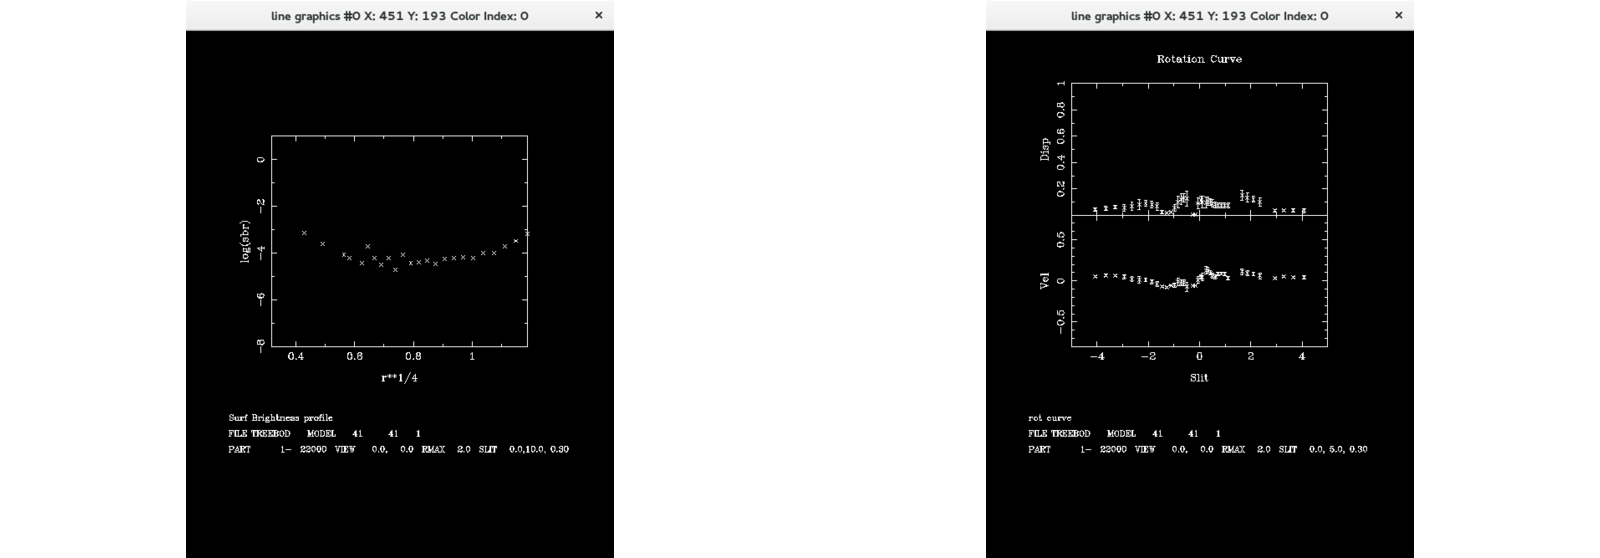
\includegraphics[scale=0.3]{norarotsbr2.png}
 \caption{\emph{El brillo superficial a radio mayor calculado en nora es mayor que debería para que sea una función lineal con respecto a r**4, 
pero es por las partículas que se escapan. La dispersión de velocidad es ahora mayor que la velocidad de rotación. El conjunto se parece a una elíptica}}
\end{figure}

\clearpage
\paragraph{El centro de masas} se va desplazando en la dirección positiva de ox con una velocidad cási constante.(cuando se crea el modelo inicial: en t=0 con setorb los 2 objetos están aliniados en la dirección ox, el centro de masas de los 2 objetos está casi en el origen y a la velocidad de todas las particulas le añade $-\vec{vr}/2 $ (el signo negativo porque van hacía el centro), pero el objeto con disco que es 10 veces más masivo  está situado en la parte negativa de ox y el modelo esférico en la parte positiva)


\begin{figure}[!ht]
 \centering
 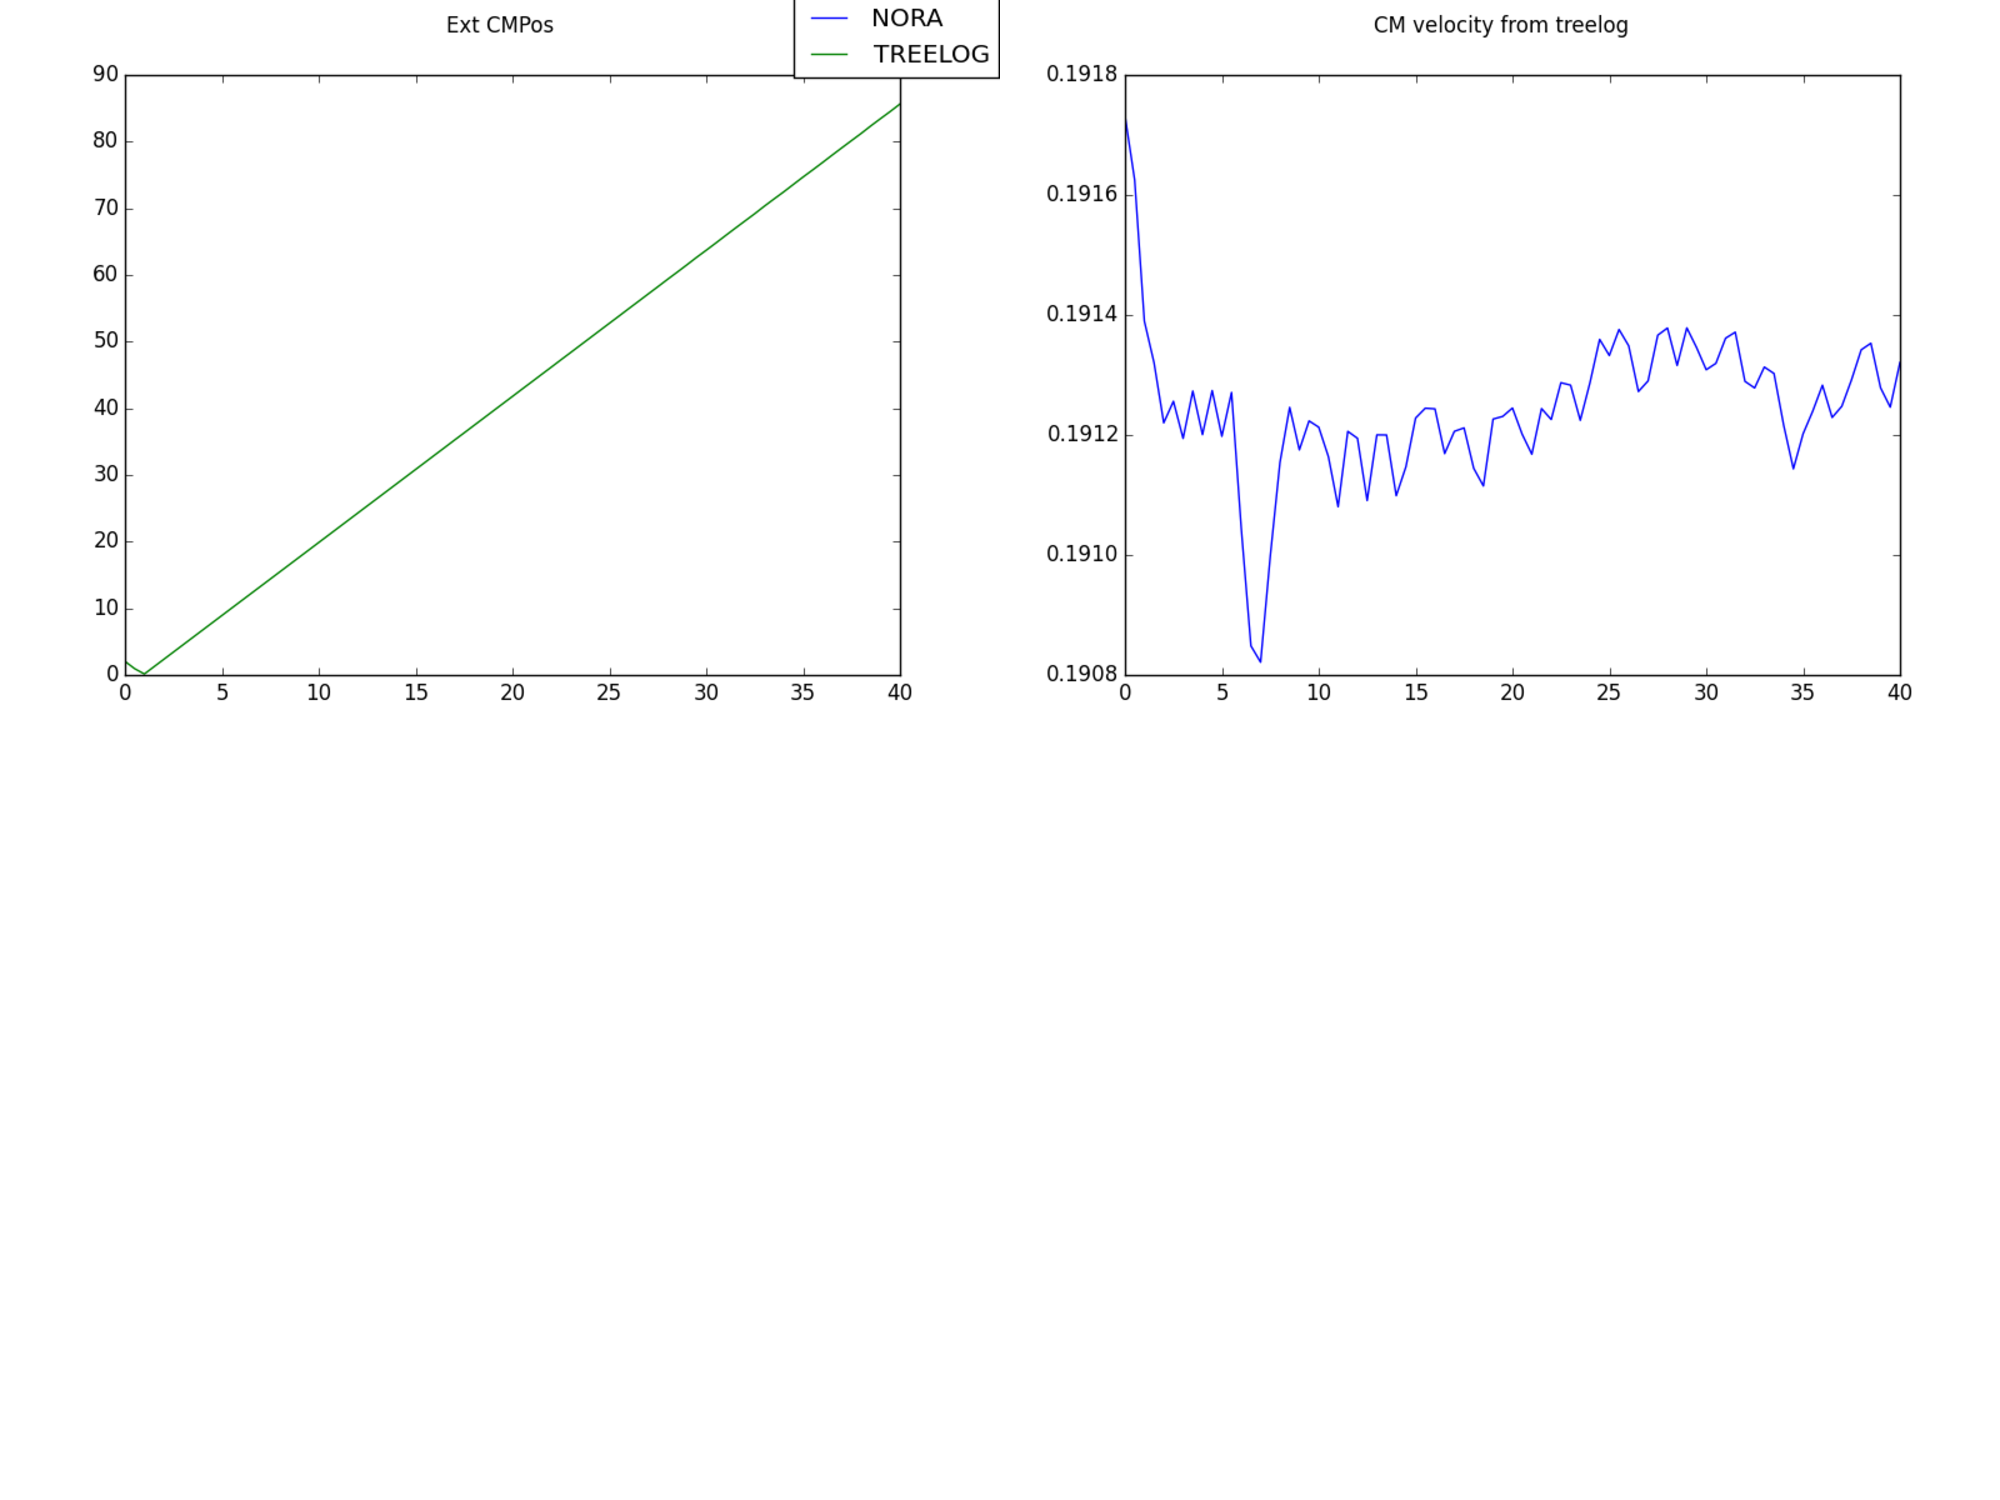
\includegraphics[scale=0.2]{cmpos-vel.png}
 \caption{\emph{la distancia del centro de masas con respecto al origen 
(los valores calculados con cmcent en nora son exactamente iguales a los de treelog) 
que crece lineal en el tiempo (velocidad constante) y la velocidad del centro de masas(casi constante) obtenida de treelog frente al tiempo }}
\end{figure}

\clearpage
\paragraph{La energía} total se conserva y es positiva (las particulas se escapan). Las partículas del modelo esférico que se escapan 
(y del modelo con disco, pero hay muchas menos) llevando energía cinética hacen que las demás del  sistema queden mas ligadas (después de un par de encuentros como se ve con medcent en nora los objetos están fusionados), sobre todo después del primer encuentro(cuando la energía cinética alcanza el máximo y la cola de partículas del modelo esférico se  escapa) 


\begin{figure}[!ht]
 \centering
 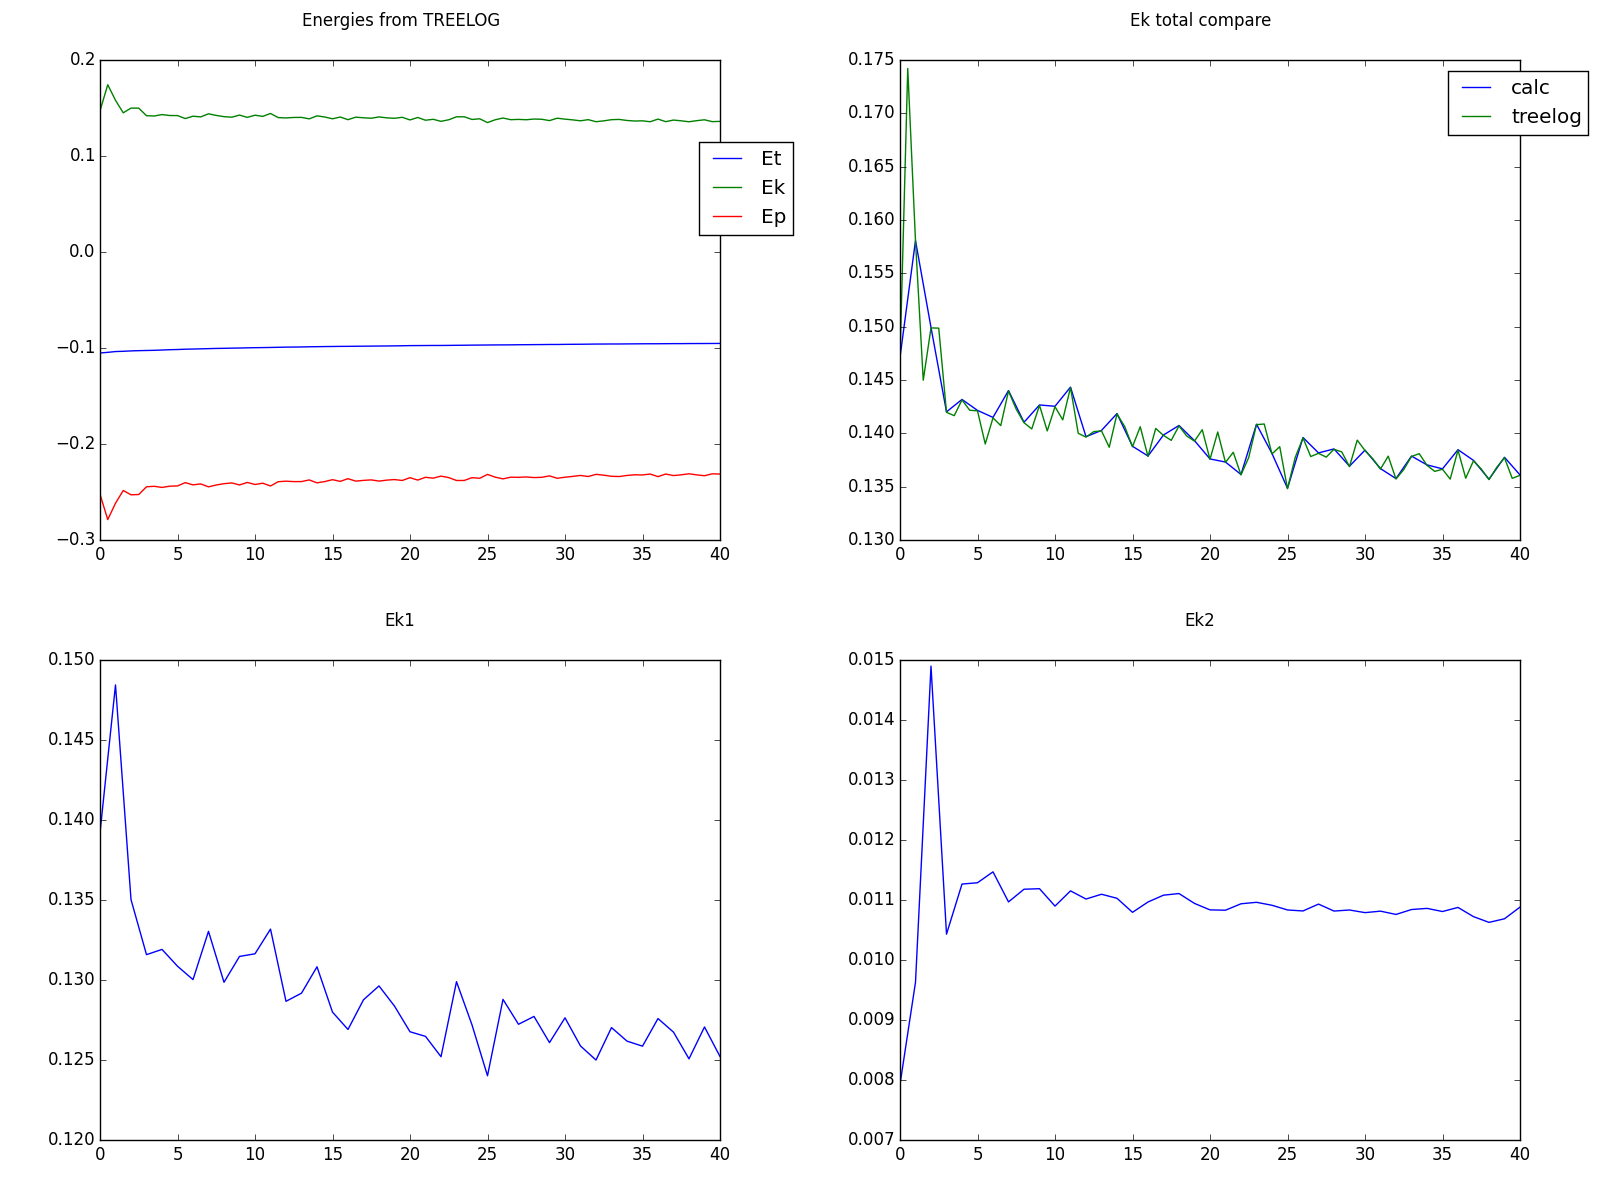
\includegraphics[scale=0.2]{sep590deg-energy.png}
 \caption{\emph{izquierda-derecha, arriba-abajo: Energias de treelog, energía cinética (comparación treelog y calculado en python - las diferencias se deben a que noutlog = 2*noutbod), energías cinéticas de los 2 objetos - todas las partículas icluyendo halos  representadas frente al tiempo}}
\end{figure}


\clearpage
\paragraph{El momento angular} del disco decrece. 
El momento angular total del sistema con 2 objetos es cási constante(se conserva).

\begin{figure}[!ht]
 \centering
 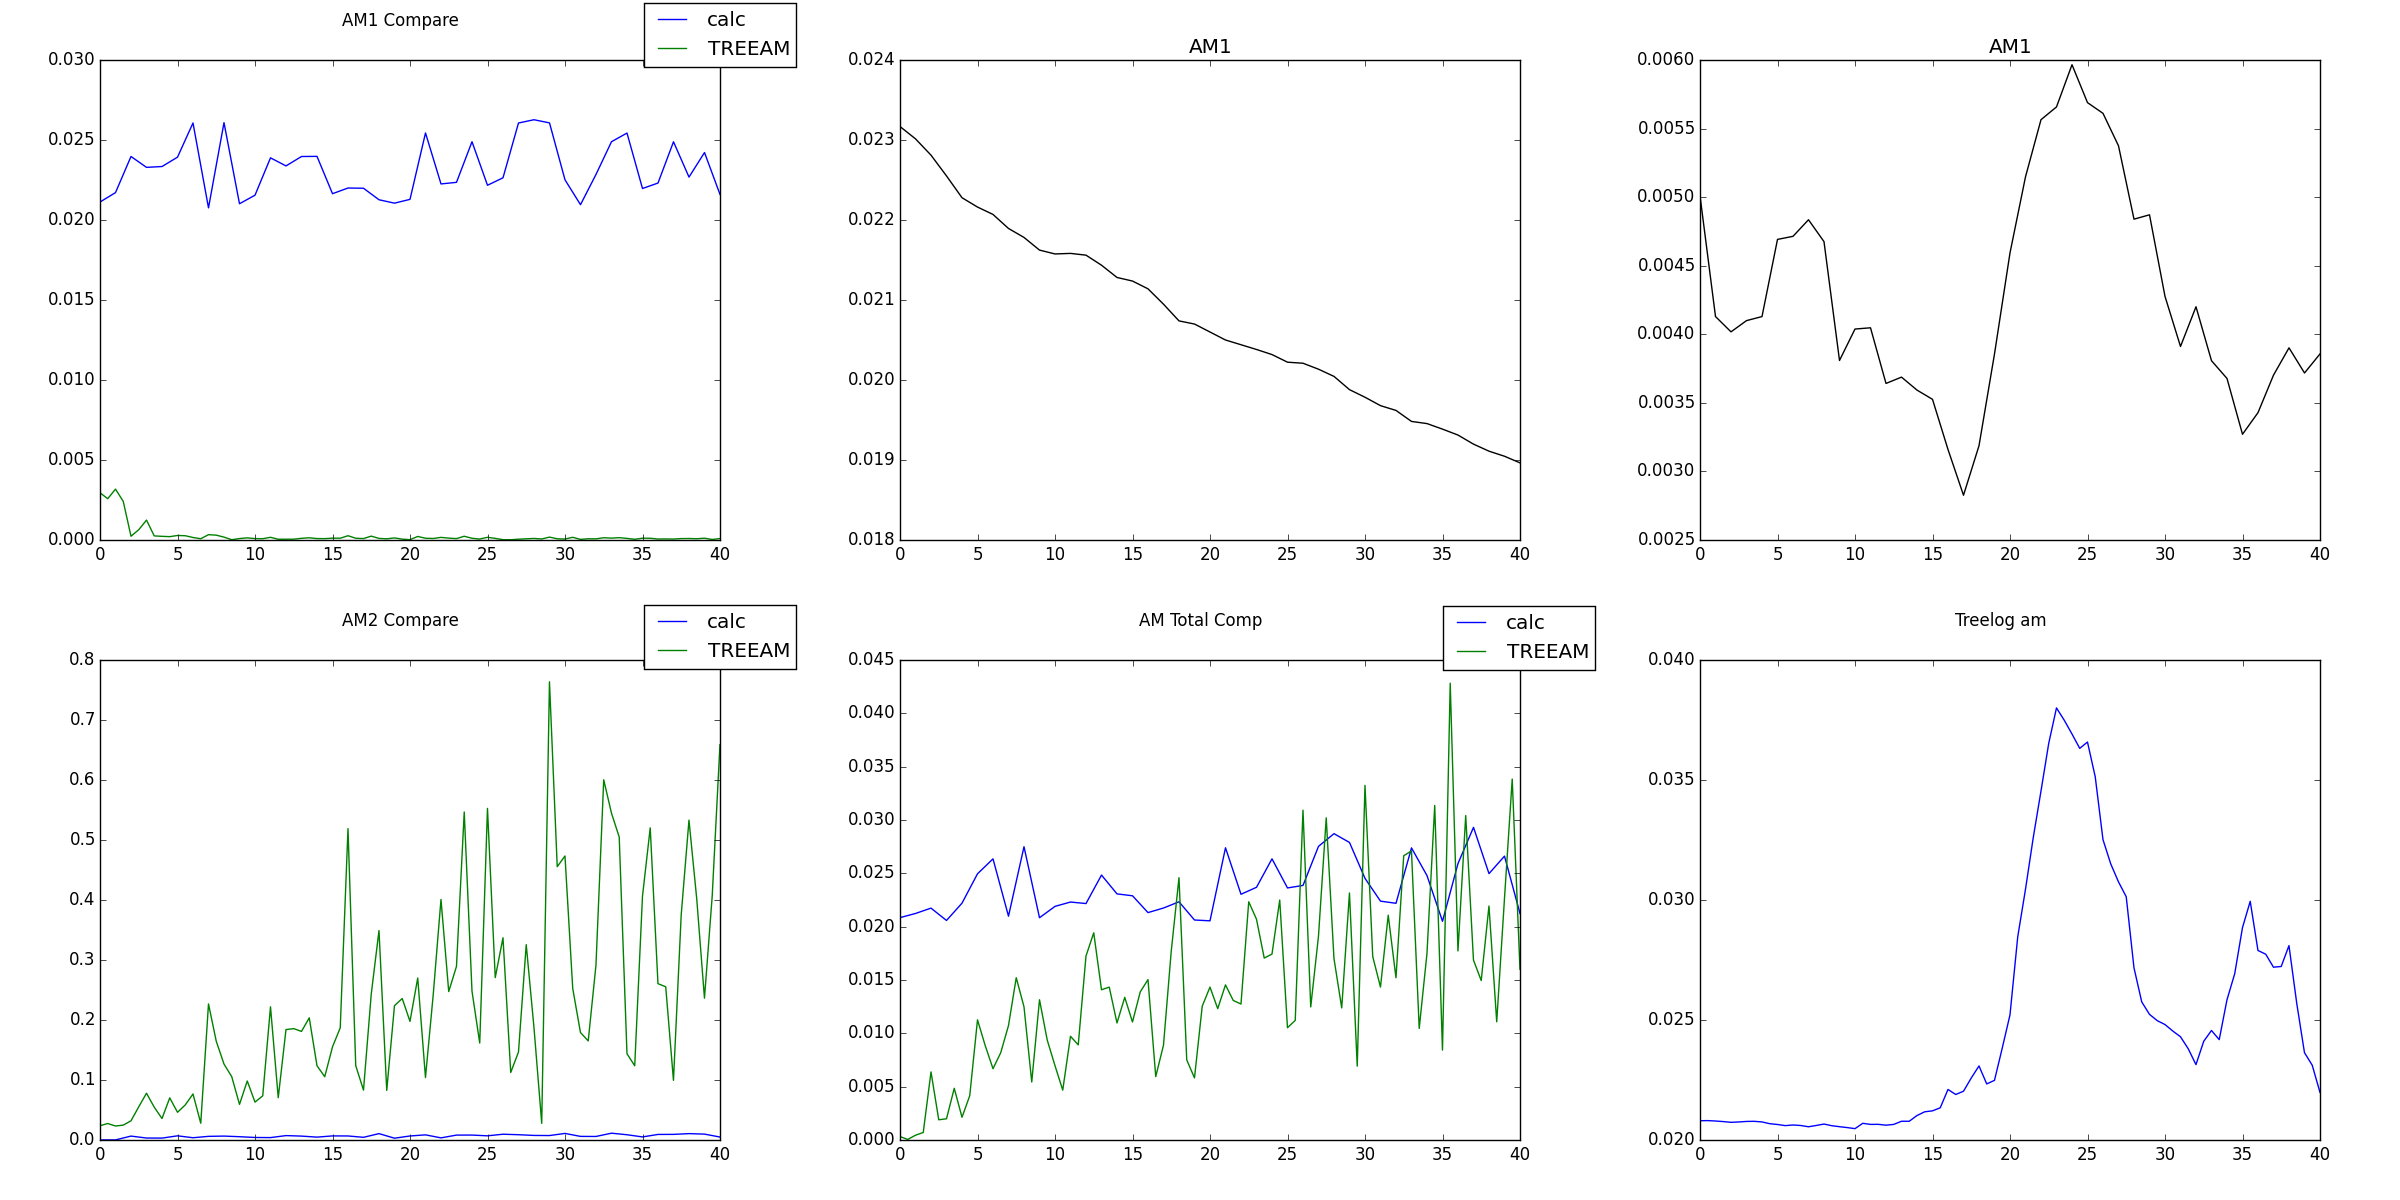
\includegraphics[scale=0.2]{sep5AM.png}
 \caption{\emph{la primera fila: am del objeto con disco(la primera columna parte luminosa+halo (comparación con TREEAM), 
segunda solo parte luminosa, tercera solo halo), la segunda fila : primera col: am del obj esférico parte luminosa+halo
(comparación conm TREEAM),  la segunda: am total(parte luminosa+halo), la tercera:  misterioso am de treelog }}
\end{figure}

En python he calculado el momento angular para cada objeto $\vec{am} = \sum_i{m_i (\vec{r_i} - \vec{cm})\times \vec{v_i}} $
donde $m_i, r_i y v_i$ son las masas, posiciones y velocidades de las partículas del objeto y cm es el centro de masa del objeto
; y de forma análoga para el momento del sistema de los 2 objetos. Los valores salen distintos de TREEAM (probablemente porque se calcularon con respecto a otro punto y no el centro de masa)

\clearpage
\newpage

\section*{Código python}


\begin{description}
\item \url{https://github.com/beevageeva/simnum2/tree/master/python/NORA}
\item makeAsc.py, nora.py, extern.py tienen que estar en la misma carpeta con los ficheros de salida de tree500 : TREE* , además los binarios xvp-asc y nora
\item determinar el numero de módelos de TREEOUT o del output de tree500
\item ejecutar 
\begin{verbatim}
	python makeAsc.py --numModels=41
\end{verbatim}
\item donde 41 es el número de modelos. Eso va a crear unos ficheros Model*.txt  que lee nora.py después
\begin{verbatim}
	python nora.py
\end{verbatim}
\item nora.py e un programa python que usa las librerías numpy, matplotlib y wx.
Se pueden seleccionar los grupos de partículas que son visibles y el objeto a que apartenece cada grupo.
Hay unos botones para cargar los modelos siguientes y anteriores.  
En el menú las funciones del submenú Each se calculan para las particulas visibles del modelo actual. 
Todas las funciones de los submenús  Each y All(calc) y  las funciones que calculan RM y Center (of mass) distance se van a  calcular solo para las partículas visibles, los que calculan momento angular y energía en los submenús All(ext) y All(comp)  se calculan para todas las particulas. 
La explicación es que el momento angular y energía calculados con las herramientas externas (ver extern.py) 
son valores de los ficheros de salida TREEAM y TREELOG, pero los valores obtenidos con Rm , 
medcent y cmcent que se ejecutan en nora se pueden calcular para un cierto rango (bodsrange). 

Las funciones del submenú All(calc) pueden tardar un poco porque se calculan para todos los modelos: se usan ficheros *.txt donde se guardan los valores para no calcularlas siempre, también para algunos calculos en nora: ver el parámetro useCalcValues = True  (y donde se usa) en nora.py y extern.py. 
Los videos se han obtenido de las imagenes generadas con la función Make images del submenú All(calc).
Pulsando en una particula(onpick event) se va a representar el vector de la velocidad(multiplicado por una constante que por defecto es 10, se puede cambiar con el slider).
Hay 2 sliders que representan el valor con cual se multiplica el módulo de la velocidad y momento angular en un instante (en el submenú Each).
Mirar también el output del programa

\end{description}


\end{document}
